%% abtex2-modelo-trabalho-academico.tex, v-1.8 laurocesar
%% Copyright 2012-2013 by abnTeX2 group at http://abntex2.googlecode.com/ 
%%
%% This work may be distributed and/or modified under the
%% conditions of the LaTeX Project Public License, either version 1.3
%% of this license or (at your option) any later version.
%% The latest version of this license is in
%%   http://www.latex-project.org/lppl.txt
%% and version 1.3 or later is part of all distributions of LaTeX
%% version 2005/12/01 or later.
%%
%% This work has the LPPL maintenance status `maintained'.
%% 
%% The Current Maintainer of this work is the abnTeX2 team, led
%% by Lauro César Araujo. Further information are available on 
%% http://abntex2.googlecode.com/
%%
%% This work consists of the files abntex2-modelo-trabalho-academico.tex,
%% abntex2-modelo-include-comandos and abntex2-modelo-references.bib
%%

% ------------------------------------------------------------------------
% ------------------------------------------------------------------------
% abnTeX2: Modelo de Trabalho Academico (tese de doutorado, dissertacao de
% mestrado e trabalhos monograficos em geral) em conformidade com 
% ABNT NBR 14724:2011: Informacao e documentacao - Trabalhos academicos -
% Apresentacao
% ------------------------------------------------------------------------
% ------------------------------------------------------------------------

\documentclass[
	% -- opções da classe memoir --
	11pt,				% tamanho da fonte
	openright,			% capítulos começam em pág ímpar (insere página vazia caso preciso)
	oneside,			% twoside para impressão em verso e anverso. Oposto a oneside
	a4paper,			% tamanho do papel. 
	% -- opções da classe abntex2 --
	%chapter=TITLE,		% títulos de capítulos convertidos em letras maiúsculas
	%section=TITLE,		% títulos de seções convertidos em letras maiúsculas
	%subsection=TITLE,	% títulos de subseções convertidos em letras maiúsculas
	%subsubsection=TITLE,% títulos de subsubseções convertidos em letras maiúsculas
	% -- opções do pacote babel --
	english,			% idioma adicional para hifenização
	french,				% idioma adicional para hifenização
	spanish,			% idioma adicional para hifenização
	brazil,				% o último idioma é o principal do documento
	]{abntex2}

\usepackage{abntex2-cefetmg-timoteo}

% ---
% PACOTES
% ---

% ---
% Pacotes fundamentais 
% ---
\usepackage{cmap}				% Mapear caracteres especiais no PDF
\usepackage{lmodern}			% Usa a fonte Latin Modern			
\usepackage[T1]{fontenc}		% Selecao de codigos de fonte.
\usepackage[utf8]{inputenc}		% Codificacao do documento (conversão automática dos acentos)
\usepackage{lastpage}			% Usado pela Ficha catalográfica
\usepackage{indentfirst}		% Indenta o primeiro parágrafo de cada seção.
\usepackage{color}				% Controle das cores
\usepackage{graphicx}			% Inclusão de gráficos
\PassOptionsToPackage{normalem}{ulem} % Para não usar sublinhado em referências bibliográficas
\usepackage{ulem}
\usepackage{multicol}
% ---

%Trocar fonte para Arial ou Helvetica
%\usepackage{uarial}
\usepackage{helvet}
\renewcommand{\familydefault}{\sfdefault}

		
% ---
% Pacotes adicionais, usados apenas no âmbito do Modelo Canônico do abnteX2
% ---
%\usepackage{lipsum}				% para geração de dummy text
% ---

% ---
% Pacotes de citações
% ---
\usepackage[brazilian,hyperpageref]{backref}	 % Paginas com as citações na bibl
\usepackage[alf,abnt-thesis-year=both,]{abntex2cite}	% Citações padrão ABNT


%Outros pacotes

\usepackage{longtable}


%\setlrmarginsandblock{3cm}{2cm}{*}
%\setulmarginsandblock{3cm}{2cm}{*}
%\checkandfixthelayout


% --- 
% CONFIGURAÇÕES DE PACOTES
% --- 

% ---
% Configurações do pacote backref
% Usado sem a opção hyperpageref de backref
\renewcommand{\backrefpagesname}{Citado na(s) página(s):~}
% Texto padrão antes do número das páginas
\renewcommand{\backref}{}
% Define os textos da citação
\renewcommand*{\backrefalt}[4]{
	\ifcase #1 %
		Nenhuma citação no texto.%
	\or
		Citado na página #2.%
	\else
		%Citado #1 vezes nas páginas #2.%
		Citado nas páginas #2.%
	\fi}%
% ---


% ---
% Informações de dados para CAPA e FOLHA DE ROSTO
% ---
\titulo{Análise de desempenho de uma implementação de Unidade de Memorização de Traços Dinâmicos em FPGA}
\autor{Elias Luiz da Silva Júnior}
\local{Timóteo}
\data{2016}
\orientador{Bruno Rodrigues Silva}
%\coorientador{Beltrano de Silva e Tal}
\instituicao{%
  Centro Federal de Educação Tecnológica de Minas Gerais
  \par
  Campus Timóteo
  \par
  Graduação em Engenharia de Computação
}
\tipotrabalho{Trabalho de conclusão de curso (Graduação)}
% O preambulo deve conter o tipo do trabalho, o objetivo, 
% o nome da instituição e a área de concentração 

%\preambulo{Proposta de pesquisa apresentada à Coordenação de Engenharia de Computação do Campus Timóteo do Centro Federal de Educação Tecnológica de Minas Gerais para obtenção do grau de Bacharel em Engenharia de Computação.}

\preambulo{Monografia apresentada à Coordenação de Engenharia de Computação do Campus Timóteo do Centro Federal de Educação Tecnológica de Minas Gerais para obtenção do grau de Bacharel em Engenharia de Computação.}

% ---

% ---
% Configurações de aparência do PDF final

% informações do PDF
\makeatletter
\hypersetup{
     	%pagebackref=true,
		pdftitle={\@title}, 
		pdfauthor={\@author},
    	pdfsubject={\imprimirpreambulo},
	    pdfcreator={LaTeX with abnTeX2},
		pdfkeywords={abnt}{latex}{abntex}{abntex2}{trabalho acadêmico}, 
		colorlinks=true,       		% false: boxed links; true: colored links
    	linkcolor=black,          	% color of internal links
    	citecolor=black,        		% color of links to bibliography
    	filecolor=black,      		% color of file links
		urlcolor=black,
		bookmarksdepth=4
}
\makeatother
% --- 

% --- 
% Espaçamentos entre linhas e parágrafos 
% --- 

% O tamanho do parágrafo é dado por:
\setlength{\parindent}{1.3cm}

% Controle do espaçamento entre um parágrafo e outro:
\setlength{\parskip}{0.2cm}  % tente também \onelineskip

% ---
% compila o indice
% ---
\makeindex
% ---

% ----
% Início do documento
% ----
\begin{document}

% Retira espaço extra obsoleto entre as frases.
\frenchspacing 

% ----------------------------------------------------------
% ELEMENTOS PRÉ-TEXTUAIS
% ----------------------------------------------------------
 \pretextual

% ---
% Capa
% ---
\imprimircapa
% ---

% ---
% Folha de rosto
% (o * indica que haverá a ficha bibliográfica)
% ---
\imprimirfolhaderosto*
% ---

% ---
% Inserir a ficha bibliografica
% ---

% Isto é um exemplo de Ficha Catalográfica, ou ``Dados internacionais de
% catalogação-na-publicação''. Você pode utilizar este modelo como referência. 
% Porém, provavelmente a biblioteca da sua universidade lhe fornecerá um PDF
% com a ficha catalográfica definitiva após a defesa do trabalho. Quando estiver
% com o documento, salve-o como PDF no diretório do seu projeto e substitua todo
% o conteúdo de implementação deste arquivo pelo comando abaixo:
%
% \begin{fichacatalografica}
%		\includegraphics{inclusao-fichaCatalografica.pdf}
% \end{fichacatalografica}
%\begin{fichacatalografica}
%	\vspace*{\fill}					% Posição vertical
%	\hrule							% Linha horizontal
%	\begin{center}					% Minipage Centralizado
%	\begin{minipage}[c]{12.5cm}		% Largura
%	
%	\imprimirautor
%	
%	\hspace{0.5cm} \imprimirtitulo  / \imprimirautor. --
%	\imprimirlocal, \imprimirdata-
%	
%	\hspace{0.5cm} \pageref{LastPage} p. : il. (algumas color.) ; 30 cm.\\
%	
%	\hspace{0.5cm} \imprimirorientadorRotulo~\imprimirorientador\\
%	
%	\hspace{0.5cm}
%	\parbox[t]{\textwidth}{\imprimirtipotrabalho~--~\imprimirinstituicao,
%	\imprimirdata.}\\
%	
%	\hspace{0.5cm}
%		1. Palavra-chave1.
%		2. Palavra-chave2.
%		I. Orientador.
%		II. Universidade xxx.
%		III. Faculdade de xxx.
%		IV. Título\\ 			
%	
%	\hspace{8.75cm} CDU 02:141:005.7\\
%	
%	\end{minipage}
%	\end{center}
%	\hrule
%\end{fichacatalografica}
% ---

% ---
% Inserir errata
% ---
%\begin{errata}
%Elemento opcional da \citeonline[4.2.1.2]{NBR14724:2011}. Exemplo:

%\vspace{\onelineskip}

%FERRIGNO, C. R. A. \textbf{Tratamento de neoplasias ósseas apendiculares com
%reimplantação de enxerto ósseo autólogo autoclavado associado ao plasma
%rico em plaquetas}: estudo crítico na cirurgia de preservação de membro em
%cães. 2011. 128 f. Tese (Livre-Docência) - Faculdade de Medicina Veterinária e
%Zootecnia, Universidade de São Paulo, São Paulo, 2011.

%\begin{table}[htb]
%\center
%\footnotesize
%\begin{tabular}{|p{1.4cm}|p{1cm}|p{3cm}|p{3cm}|}
%  \hline
%   \textbf{Folha} & \textbf{Linha}  & \textbf{Onde se lê}  & \textbf{Leia-se}  \\
%    \hline
%    1 & 10 & auto-conclavo & autoconclavo\\
%   \hline
%\end{tabular}
%\end{table}

%\end{errata}
% ---

% ---
% Inserir folha de aprovação
% ---

% Isto é um exemplo de Folha de aprovação, elemento obrigatório da NBR
% 14724/2011 (seção 4.2.1.3). Você pode utilizar este modelo até a aprovação
% do trabalho. Após isso, substitua todo o conteúdo deste arquivo por uma
% imagem da página assinada pela banca com o comando abaixo:
%
%\includegraphics[width=1\textwidth]{inclusao-folhaDeAprovacao.pdf}
%\includegraphics[width=1\textwidth]{inclusao-ata.pdf}



.

.

.



%
% ---

% ---
% Dedicatória
% ---
%\begin{dedicatoria}
%    \vspace*{\fill}
%	\begin{flushright}
%		Dedico a\\
%		algumas pessoas.
%	\end{flushright}
%\end{dedicatoria}
%% ---
%
%% ---
%% Agradecimentos
%% ---
%\begin{agradecimentos}
%
%Agradeço aos pais no primeiro parágrafo?
%
%E à namorada ou ao namorado no segundo?
%
%Orientador no terceiro?
%
%Esta página de agradecimentos vive dando problemas.
%
%\end{agradecimentos}
%% ---
%
%% ---
%% Epígrafe
%% ---
%\begin{epigrafe}
%    \vspace*{\fill}
%	\begin{flushright}
%		\textit{``Os grandes navegadores \\devem sua reputação aos temporais e tempestades''.\\
%		Epicuro}
%	\end{flushright}
%\end{epigrafe}



% ---

% ---
% RESUMOS
% ---

% resumo em português
\setlength{\absparsep}{18pt} % ajusta o espaçamento dos parágrafos do resumo
\begin{resumo}

\noindent 
%Um único parágrafo que sintetize todo o meu trabalho. Organização de informação usando classificação facetada é útil para melhorar a indexação de documentos e a construção de sistemas de recuperação de informação corporativa. Essa hipótese baseia-se na evidência de facetas comuns a documentos de diferentes empresas e na flexibilidade da organização facetada. Entretanto, a classificação e indexação automáticas de um grande volume de documentos representam importantes obstáculos e nossa principal motivação. A pesquisa é descritiva, aplicada e experimental e tenta responder sobre a existência de características comuns a documentos do domínio corporativo e a possibilidade de indexação facetada automática. Duas coleções são usadas para avaliação, uma pública e outra particular. Os termos usados por autores de documentos foram obtidos através de documentos e expressões de busca. Foi empreendida uma análise preliminar do domínio corporativo, pela qual foram descobertas 12 categorias comuns e facetas úteis para o contexto de cada coleção de avaliação. A distribuição de assuntos em categorias apresentou alta correlação positiva usando o coeficiente de correlação de Spearman. Dez expressões de busca de usuários foram avaliadas no contexto da coleção particular e validaram as 12 categorias comuns. A avaliação empírica da trilha \textit{Enterprise} da \textit{Text Retrieval Conference} foi executada e os métodos de indexação, classificação e recuperação automáticos de informação facetada melhoraram a eficiência da recuperação sem fazer uso de serviços externos, como Wikipedia e metabuscadores, e sem fazer uso de estruturas hipertextuais presentes nos documentos da amostra. A avaliação empírica utilizou-se principalmente das características espaciais, temporais, de documento e de pessoal. A técnica de análise facetada mostrou-se promissora para os métodos de análise e comparação de coleções corporativas sem que dados puros sejam expostos a terceiros. A tese aponta direções de pesquisa para o uso dos métodos em outras coleções, para aperfeiçoamentos da organização da informação facetada, e para novas aplicações dos métodos também em outros domínios.

\noindent 
\textbf{Palavras-chave}: %análise de domínio, análise facetada, recuperação de informação, informação corporativa.

\end{resumo}

% resumo em inglês
\begin{resumo}[Abstract]
 \begin{otherlanguage*}{english}

\noindent 
%We hypothesise that information organisation based on faceted classification is useful to improve enterprise information retrieval systems. The existence of similar facets in documents from different companies and the known adaptability of facet organisation strengthen this hypothesis. We refer this work to the automated classification and indexing on large amounts of text files. This work is descriptive, applied, and experimental. It aimed to expose the main characteristics of the enterprise information, proposing a tentative generalisation to the enterprise domain and presenting some facets we can use to organise it and to support better information retrieval. It applied facet analysis to two enterprise collections and evaluated the resulting faceted classification. Terms were selected from documents and queries. We found twelve common categories and the distribution of document subjects across the categories presents strong positive correlation by the Spearman’s rank correlation. Then, we obtained ten user queries and we adopted them to validate the found categories. We also used the Enterprise track of Text Retrieval Conference and its previous results as a Cranfield-like evaluation. The automated prototype used spatial, temporal, document and social characteristics. Thus, our empirical evaluation improved the information retrieval with no external dependency like Wikipedia or metasearch engines. The facet analysis was useful for comparing the companies with no desire to expose their information. The method can guide and stimulate future work and other companies can become more willing to take part in a research study.

\noindent  
   \textbf{Keywords}: %domain analysis, facet analysis, information retrieval, enterprise information.
 \end{otherlanguage*}
\end{resumo}

% ---
% inserir lista de ilustrações
% ---

%%%% no extra space before the entry, or in the LoF/LoT
%% \setlength{\cftbeforechapterskip}{0pt plus 0pt} %afeta sumário, o que não desejo!
% \renewcommand*{\insertchapterspace}{} %afeta apenas lista de figuras e lista de tabelas, precisamente o que desejo!
%
%\pdfbookmark[0]{\listfigurename}{lof}
%\listoffigures*
%\cleardoublepage
%% ---
%
%% ---
%% inserir lista de tabelas
%% ---
%\pdfbookmark[0]{\listtablename}{lot}
%\listoftables*
%\cleardoublepage
%% ---
%
%% ---
%% inserir lista de abreviaturas e siglas
%% ---
%%\begin{siglas}
%%  \item[Fig.] Area of the $i^{th}$ component
%%  \item[456] Isto é um número
%%  \item[123] Isto é outro número
%%  \item[lauro cesar] este é o meu nome
%%\end{siglas}
%% ---
%
%% ---
%% inserir lista de símbolos
%% ---
%%\begin{simbolos}
%%  \item[$ \Gamma $] Letra grega Gama
%%  \item[$ \Lambda $] Lambda
%%  \item[$ \zeta $] Letra grega minúscula zeta
%%  \item[$ \in $] Pertence
%%\end{simbolos}
%% ---

% ---
% inserir o sumario
% ---
\pdfbookmark[0]{\contentsname}{toc}
\tableofcontents*
\cleardoublepage
% ---



% ----------------------------------------------------------
% ELEMENTOS TEXTUAIS
% ----------------------------------------------------------
\textual

% ----------------------------------------------------------
% Introdução
% ----------------------------------------------------------
\chapter[Introdução]{Introdução}

%\chapter{Introdução}

	\begin{flushright}
		\textit{``Clássico é clássico e vice-versa''.\\
		Mário Jardel}
	\end{flushright}


%\textbf{Organização de informação não se dá da mesma forma em qualquer domínio.}
%As metodologias e técnicas tradicionais de organização de informação (OI) permitem que informação seja coletada, indexada, classificada e recuperada, na Web ou em outros repositórios, tendo em vista seu consequente uso por uma comunidade de usuários. No entanto, é comum a necessidade de se implementar métodos com foco em repositórios e conteúdos de áreas específicas, por aqueles métodos tradicionais não suportarem o reconhecimento de termos de todos os domínios ou não atenderem a necessidades muito específicas dos usuários de informação. Esse é o caso do tratamento de fórmulas químicas \cite{sun07}, de citações bibliográficas \cite{giles98} e de referências geográficas \cite{overellPhd09}, assim como de repositórios de patentes \cite{patents11} e de informação corporativa \cite{hu2010enterprisecase}.
%
%%\textbf{SRIC ainda costumam ser SRI sem qualquer adaptação especial.}
%Porém, ainda é comum que sistemas de recuperação de informação corporativa sejam apenas sistemas tradicionais de recuperação de informação sobre repositórios de documentos corporativos. 
%Dessa forma, apenas pequena parcela da tecnologia é adaptada para atender as necessidades das empresas e de seus usuários. 
%Isso frequentemente leva a insatisfação de usuários de informação e causa prejuízos aos processos organizacionais que dependam de buscas \cite{solomon2002}.
%
%%\textbf{O usuário costuma precisar de vários SRI para realizar a mesma tarefa.}
%Adicionalmente, as tarefas de usuários corporativos normalmente exigem informação de diferentes fontes de informação \cite{halevy2005enterprise}, tornando comum o acesso a tais fontes por meio de diferentes sistemas de recuperação de informação. 
%Apesar de complexo, o acesso através de uma única e integrada interface é muito importante para qualquer usuário de informação, além de recomendável para garantir uma gestão eficaz de recursos de informação.
%
%%\textbf{Tudo isso é culpa da complexidade da informação corporativa. Conhecê-la melhor é a solução.}
%Essas dificuldades são comuns em decorrência da complexidade naturalmente encontrada dentro de organizações, onde diferentes profissionais, atividades e unidades organizacionais são empregados para realizar trabalho. A recuperação mais eficaz de informação corporativa e o desenvolvimento de metabuscas mais eficientes parecem depender da compatibilização e do controle de características que permeiem a informação da empresa, o que sintetiza a justificativa desta pesquisa.

A Lei de Moore possui algumas variações quanto ao seu enunciado, porém todas afirmam que a capacidade computacional dos processadores cresceria exponencialmente devido aos avanços na tecnologia. Por 50 anos essa previsão se manteve consistente com os produtos lançados no mercado, como descrito em. Porém, limitações físicas na criação de circuitos integrados ameaçam o continuidade dessa evolução. \cite{50yearsmooreslaw}

Mas com o crescente aumento da demanda por computação é necessário que os projetistas encontrem maneiras de aperfeiçoar ainda mais o funcionamento das unidades de processamento. Uma solução que vem sendo utilizada é acoplar vários processadores para funcionar em paralelo, porém isso aumenta a complexidade de projetos tanto a nível de hardware como de software, além de amplificar o consumo energético do sistema.

O grande desafio da arquitetura de computadores é buscar soluções eficientes, conciliando fatores como desempenho do sistema, consumo de energia, custo de produção e tamanho e complexidade do produto final. Em muitas situações, esses fatores concorrem entre si, levando o projetista a ter de tomar decisões sobre qual abordagem será escolhida para solucionar determinado problema.

O que ocorre então é a criação de sistemas especialistas para determinadas funções, enquanto outros projetos mais gerais lidam com uma gama mais diversa de aplicações. Em ambos os casos, projetistas consideram qual problema buscam resolver para criar a solução mais adequada dentro das restrições. 

Como exemplo podemos comparar as diferentes abordagens assumidas ao projetar um \textit{system-on-chip} para aplicação em um sistema embarcado e na criação de uma unidade de processamento gráfico. Enquanto sistemas embarcados prezam por tamanho reduzido e baixo consumo de energia, unidades gráficas têm como prioridade a velocidade para cálculos de ponto flutuante, sendo otimizadas para executar instruções simples a diversos dados de entrada simultaneamente. \cite{tanenbaumsco}




\section{Justificativa} %Inseri para organizar o texto

%\textbf{Necessidade de SRI adequados para informação corporativa, que evoluam continuamente e que busquem a generalidade.}
Esta pesquisa justifica-se pela necessidade de se implementar sistemas automáticos de recuperação de informação que deem suporte adequado à informação corporativa e às tarefas dos usuários corporativos, mas também que favoreçam a provisoriedade da informação e a interoperabilidade entre sistemas. Para isso, deve-se buscar uma compreensão mais geral da informação corporativa, que beneficie sua evolução contínua e não a limite a um cenário de uso excessivamente reduzido.

%\textbf{Há diversas iniciativas para aumentar o desempenho dos componentes dos SRI.}
Há diversas iniciativas que tentam aumentar o desempenho dos componentes de sistemas de recuperação de informação corporativa e dos processos que os suportam, da coleta de documentos à interface com o usuário. As iniciativas mais comuns dependem de vocabulário controlado \cite{ontology12}, o que nem sempre é simples de gerir dentro de empresas. A adoção de vocabulário controlado enfrenta um grande volume de informação produzida, a dificuldade de avaliar a conformidade de novos documentos, e ainda a realidade de que nem toda empresa conta com profissionais de informação qualificados, sendo que suas funções eventualmente são assumidas pelos próprios usuários corporativos. Adicionalmente, nem todo usuário de informação possui habilidades suficientes para executar atividades de produção, classificação, indexação e busca de informação da forma mais eficiente.
Outras iniciativas dependem de relacionamentos entre documentos em forma hipertextual, assim como ocorre na \textit{Web}. Esse não é um recurso muito comum em coleções corporativas, onde memorandos, notas fiscais, manuais, folhas de pagamento e balanços são conectados apenas através de códigos textuais, nem sempre fáceis de se reconhecer automaticamente.

%\textbf{Maioria das iniciativas dão-se sobre a perspectiva dos projetistas ou sobre a perspectiva dos usuários, o que gera dois problemas: ou requer um projeto prévio intenso ou perde em flexibilidade para evolução.}
No entanto, a maioria dessas iniciativas continua a ser fortemente dependente da perspectiva dos projetistas dos sistemas de recuperação de informação, com reflexos provenientes da forma como a informação é estruturada nos diversos repositórios usados pela empresa; ou da perspectiva dos usuários, com reflexos provenientes da forma como o conhecimento é organizado. Embora natural, essa dependência exige um grande esforço prévio de projeto ou então provoca uma excessiva perda de flexibilidade para a evolução do sistema de recuperação de informação. 

%\textbf{Estruturas classificatórias facetadas resolvem os dois problemas anteriores.}
Para contornar essas limitações, estruturas classificatórias facetadas têm sido adotadas como base para um modelo mais flexível e incremental de desenvolvimento de sistemas de recuperação de informação \cite{broughton2006,docubrowse10}. Adicionalmente, uma vez que documentos apresentam facetas significativas para o contexto do documento e do usuário da informação, normalmente consultas submetidas aos mecanismos de busca também incluem estas facetas, como nomes de pessoas e de instituições, localidades e datas \cite{rosieJones08,docubrowse10,mir2ed}. Tal contextualização, além de favorecer a recuperação de informação, pode contribuir para melhorar o \textit{ranking} da informação e para criar novos serviços e funcionalidades \cite{borges07}.

%A origem da classificação facetada se deu com estudos de \citeonline{ranganathan1967} e teve continuidade nos estudos de outros autores da área de Biblioteconomia e Ciência da Informação tais como \citeonline{vickery2008faceted} e \citeonline{broughton2006}, apesar do conceito estar em uso crescente também em outras áreas com algumas variações \cite{broughton2006}. As facetas identificadas a partir desta pesquisa constituem características comuns da informação corporativa de duas empresas, mas favorecem a análise de um domínio corporativo na medida em que o método pode ser repetido em organizações adicionais, usando documentos de diferentes tipos, propósitos e idiomas. 

%Na teoria da análise facetada de \citeonline{ranganathan1967}, faceta é um conceito central, embora apresente interpretações variadas na literatura \cite{broughton2006}. No entanto, faceta sempre é vista como uma característica permanente e relevante de uma entidade, algumas vezes reconhecida por meio da análise facetada. Análise facetada é uma técnica através da qual facetas são descobertas em um domínio e normalmente formam uma classificação facetada \cite{labarre2010}. A abordagem facetada constitui uma estratégia classificatória pela qual se procura responder como uma entidade pode ser descrita, ao invés de procurar responder onde a entidade deve ser posicionada dentro de uma estrutura classificatória definida \textit{a priori} \cite{ranganathan1967}. Assim, variadas perspectivas e incertezas sobre necessidades de usuários são consideradas, dentro de um processo analítico, incremental e iterativo, normalmente tornando seu produto útil para mais de um problema.

%\textbf{Facetas significativas são descobertas por uma análise de domínio.}
As facetas mais significativas do domínio corporativo podem ser descobertas através de um processo de análise de domínio. E por meio de facetas significativas, a organização da informação pode ser aperfeiçoada e sistemas de recuperação de informação mais eficientes são possíveis \cite{albrechtsen1993subject}. Porém, os requisitos para a análise de todo um domínio e para a análise da informação de uma única empresa são diferentes \cite{gopinath92}. Enquanto o domínio requer uma compreensão mais geral e consensual, a informação de uma instituição admite perspectivas baseadas em maior empirismo e pragmatismo, sendo útil apenas em um contexto mais limitado \cite{hjorland2002domain}.

%\textbf{Análise de domínio deve ser cuidadosa para reconhecer as características essenciais.}
As facetas normalmente restringem-se às mais importantes por razões econômicas e práticas mesmo havendo muitas características potencialmente relevantes ao domínio \cite{ranganathan1967}. É possível descobrir características do domínio através de técnicas como da análise facetada. No entanto, distinguir entre características importantes e essenciais só se dá através de um rigoroso processo de análise de domínio \cite{lykke2011domain}.

%\textbf{Características locais também são importantes para a análise de domínio.}
Por outro lado, as características locais da informação corporativa, a terminologia específica de uma atividade econômica, as necessidades individuais de cada unidade organizacional e o contexto geográfico e histórico da empresa também são importantes no processo de análise de domínio. Além disso, elas são úteis para descrever a informação corporativa, inclusive com uma precisão que supera aquela possibilitada por características mais gerais e genéricas. Também, as características locais são representadas da mesma forma que aquelas mais gerais do domínio \cite{dolby09extractingVocabularies,giess2008generation,wild2009describing}, mesmo não sendo compartilhadas por todas as empresas. No entanto, sua adoção implica em uma modelagem que se afasta de um modelo genérico de empresa.

%\textbf{Informação implícita também é importante.}
Em todo sistema de recuperação de informação corporativa, os usuários da informação estão interessados tanto em dados explícitos presentes no conteúdo de documentos \cite{gardin1973} quanto em informação implícita e conhecimento informal distribuído nos sistemas corporativos \cite{dealwis2001singapore,choo2008,marcella2012,nunes2006,ofarrill2010}, o que constitui um desafio adicional para a representação do domínio. Portanto, o domínio, no nível mais global ou mais individual, é dinâmico e sua representação deve estar preparada para atualizações contínuas.

%\textbf{Análise facetada se justifica como técnica para análise de domínio.}
Exatamente por favorecer um processo incremental de análise de domínio, a análise facetada parece apropriada. Porém, não há relatos da aplicação dessa técnica em documentos corporativos na literatura. Desenvolvida sobre uma base teórica sólida a partir da Biblioteconomia e da Ciência da Informação \cite{garfield1984}, a análise facetada é mais popular na sua área de origem e para a classificação bibliográfica, embora esteja se popularizando em outras áreas \cite{labarre2010}. São exemplos não exaustivos os documentos de engenharia \cite{giess2008generation,wild2009describing}, \textit{sites} corporativos \cite{wang2008using}, documentos \textit{Web} \cite{hong06,vickery2008faceted} e catálogos \textit{Web} \cite{sacco2006}. Como a diversidade de aplicações e ramos do conhecimento tem aumentado, surgem também visões alternativas e um grande número de trabalhos sem que todos os princípios originais de \citeonline{ranganathan1967} sejam respeitados \cite{spiteri98simplified,wild2009describing}.

%A análise facetada da informação corporativa, como uma técnica de análise de um domínio, deve começar por definir as facetas mais comuns e frequentes à maioria das empresas. As sugestões mais tradicionais partem das cinco categorias consideradas fundamentais por \citeonline{ranganathan1967}, personalidade, matéria, energia, espaço e tempo, e as treze recomendadas pelo \textit{Classification Research Group}: coisa, tipo, parte, propriedade, material, processo, operação, agente, paciente, produto, subproduto, espaço e tempo. Elas supostamente têm o potencial de representar o conhecimento de qualquer domínio, sendo usadas como ponto de partida para a análise facetada \cite{broughton2006}.





%\textbf{Conclusão da justificativa.}
Dessa maneira, a organização da informação por meio de estruturas classificatórias facetadas pode contribuir positivamente para a melhoria dos processos de classificação e indexação de documentos, e para outras etapas da construção e uso dos sistemas de recuperação de informação. Essa hipótese se baseia na presença de facetas comuns a documentos corporativos e na flexibilidade desse método de organização.
% Uma segunda hipótese refere-se ao relacionamento entre facetas, dentro de documentos ou mesmo dentro da coleção, como importante recurso para reconhecimento e desambiguação de termos e entidades de forma automática, o que por sua vez suportaria uma indexação automática eficiente de entidades facetadas. %Aqui pode haver um exemplo e/ou uma figura de exemplo.







%\section{Justificativa}

%Por outro lado, muito pouco se sabe da eficiência dessas técnicas de recuperação quando adotadas em conjunto, e.g. assunto, tempo e espaço \citepx{hassan09}. %Parte desse desconhecimento deve-se ao volume menor de implementações de SRI baseados em estruturas facetadas \citepx{hong06} e também ao custo de classificar grandes coleções por meio de análise facetada.

\section{Problema}

%\textbf{As questões de pesquisa.}
As seguintes questões constituem o problema desta pesquisa: 
A informação corporativa possui características que potencialmente sejam comuns a todo o domínio corporativo? 
No contexto de uso de sistemas de recuperação de informação corporativa, as expressões de busca de usuários apresentam as mesmas características que estão presentes nos documentos? 
A organização facetada da informação corporativa contribui para o aumento do desempenho geral do sistema automático de recuperação de informação?

%\textbf{Conceituação dos termos novos presentes nas perguntas acima.}
As características da informação, em documentos e expressões de busca, referem-se a atributos que devem ser reconhecidos a partir do domínio corporativo. Adicionalmente, a contribuição esperada da organização facetada da informação está associada à sua capacidade de representar entidades por meio da totalidade ou de um subconjunto de suas características, suportando a recuperação de entidades e consequentemente a recuperação de documentos onde as entidades estão contidas. Finalmente, o desempenho do sistema de recuperação de informação refere-se à sua capacidade atender às necessidades informacionais de seus usuários, algo que pode ser parcialmente medido através de métricas discutidas na literatura.

%Finalmente, a contribuição esperada da organização facetada da informação aos sistemas de recuperação de informação está associada à sua capacidade de identificar entidades por meio da totalidade ou subconjunto de seus atributos, emprestando a documentos e outras entidades parte de seu contexto.


%automaticamente termos a facetas
%aumento da precisão como medida de desempenho do SRI


%A organização multifacetada da informação demanda um esforço manual de identificação de facetas e anotação de termos da coleção ou exige um processo de reconhecimento que seja automático e suficientemente preciso para torná-la útil na recuperação de documentos.
%que caracterizam o sistema de informação corporativo pode ajudar no reconhecimento automático e na desambiguação de entidades multifacetadas e seus valores de facetas (focus)

\section{Objetivos}

%\textbf{Objetivo geral.}
Para responder ao problema proposto, o objetivo geral deste trabalho é propor um conjunto de características da informação corporativa que favoreça a organização e a recuperação da informação.
% projetar e descrever um processo de reconhecimento e desambiguação de termos que permita uma associação dinâmica entre cada termo reconhecido e sua respectiva faceta, tais como nomes de pessoas e de instituições, processos, localidades e datas.

%associação dinâmica. Como um processo automático, termo pode ser associado a uma faceta diferente daquela com a qual já se encontra associado a partir da reunião de novas evidências, pela edição de um documento ou pela simples inclusão de outros documentos no índice. Assim, a técnica deve ser aplicada recursivamente e deve ser considerada eficaz caso o número de associação falso-positiva seja baixo.

%\textbf{Objetivos específicos.}
Também, objetivam-se mais especificamente:

\begin{enumerate}
	\item Propor um conjunto de facetas que seja útil na organização automática da informação corporativa e na interoperabilidade entre diferentes repositórios de informação da mesma empresa ou de diferentes empresas;

	\item Identificar as facetas pelas quais os usuários de informação especificam sua necessidade de informação no contexto de trabalho;

	\item Avaliar as implicações da organização facetada da informação corporativa no desempenho dos sistemas automáticos de recuperação de informação.

\end{enumerate}

%\textbf{Link para os procedimentos metodológicos.}
Para responder as questões propostas e aos objetivos apresentados, pretende-se empreender uma análise preliminar do domínio corporativo a partir de dois exemplares do domínio, avaliar como os usuários informacionais mobilizam as facetas mais comuns do domínio, e implementar e avaliar um protótipo de sistema de recuperação de informação corporativa. Os procedimentos metodológicos seguidos são apresentados no capítulo \ref{metodologia}.













%\section{Contribuições esperadas}

%Pelo desenvolvimento desta pesquisa em organização de informação facetada, espera-se que sejam realizados aperfeiçoamentos em técnicas usuais de i) reconhecimento e desambiguação de termos, ii) busca de documentos por meio de consultas ambíguas, e iii) ordenação de resultados a partir de indicadores facetados.

%Na atividade de reconhecimento, o reconhecimento de termos permite a contextualização de documentos coletados para um sistema de busca, o que, em outros trabalhos, tem sido feito em classes homogêneas de documentos. Esta pesquisa pretende que documentos mais diversos, comuns em empresas, como manuais, memorandos, bancos de dados estruturados ou páginas Web sejam tratados sob o mesmo arcabouço, considerando as diferenças de gênero linguístico e ao mesmo tempo em que se possa adequadamente estendê-lo a outros idiomas. Para esse fim, deve-se implementar uma técnica de desambiguação que utilize evidências de documentos explicitamente ou implicitamente relacionados, com ou sem hipertexto, e que avalie automaticamente a qualidade da fonte de evidência de facetas.

%Para isso, deve ser implementado um protótipo funcional de sistema de recuperação de informação corporativo, com componentes de coleta, \textit{parsing}, indexação, processamento de consulta e \textit{ranking}. Tais componentes, modificados para reconhecer, desambiguar, indexar e recuperar informação multifacetada a partir dos documentos da coleção, servirão para avaliar o modelo de organização multifacetada de informação em outros cenários de teste.

%Para a atividade de busca pelo usuário, uma interface deve ser projetada para favorecer o ajuste fino dos critérios de busca, textuais e multifacetados. O método de interação com as respostas da busca pode representar um passo adiante na ordenação de respostas. Adicionalmente, um algoritmo de ordenação de documentos deve ser proposto para o mesmo arcabouço, pelo \textit{ranking} a partir dos critérios textuais e multifacetados, mas com alterações na estrutura de indexação que favoreçam o método de \textit{ranking}. Espera-se obter um algoritmo de busca eficiente por informação multifacetada, especialmente no contexto de sistemas de recuperação de informação corporativos. A avaliação da modelagem multifacetada para a organização da informação corporativa também é uma contribuição esperada.

%É necessário investigar porque as estruturas próprias não têm produzido aumento da eficiência na recuperação das respostas \cite{anastacio09}, e se isso é também verdade em buscas onde exista o ajuste fino do \textit{ranking}. É prevista a necessidade de se projetar uma estrutura de dados mais apropriada para indexar informação corporativa e multifacetada. A estrutura de dados deve privilegiar operações de atualização de índice (inclusão, alteração e exclusão de documentos da coleção) e de acesso de dados para recuperação e \textit{ranking}.

%Finalmente, os repositórios usados para avaliação de técnicas de recuperação de informação corporativa têm sido constituídos por classes similares de documentos. Logo, espera-se formar um repositório de teste e avaliação a partir de documentos de diferentes gêneros linguísticos e formatos, o que pode contribuir positivamente para pesquisas futuras. Para isso, este trabalho deve primeiramente colaborar para o projeto, criação e disponibilização de uma coleção de referência em língua portuguesa, adequado para o contexto empresarial, de fonte pública, apropriado para avaliação de SRI corporativos. A nova coleção de referência não será a única base de experimentação deste trabalho, mas sim complementar àquelas disponíveis na literatura.

%As contribuições desta pesquisa mostram-se particularmente úteis aos sistemas de RI corporativos, em qualquer idioma, mas podem igualmente ser aplicados em outros domínios. Dessa forma, não podem ser descartadas as possibilidades de se gerar produtos úteis e funcionais no curto prazo.







%\section{Resultados esperados}

%A técnica de consulta multifacetada deve favorecer a precisão e a revocação se comparada às técnicas estatísticas como TF-IDF, nosso baseline, com custo computacional conhecido.

%A técnica implementada e o método proposto devem ser mais eficientes que os baselines taxonomia facetada, TF-IDF, taxonomia facetada dinâmica, busca sobre metadados na biblioteca digital implementada em dspace.

%O desempenho também deve ser superior na coleção de referência da TREC comparada com resultados disponíveis na literatura.









\section{Estrutura da tese}

%\textbf{Links para os próximos capítulos.}
Esta tese está estruturada em seis capítulos, ordenados pelo momento em que foram concluídos dentro do ciclo de vida desta pesquisa, e anexos, a saber:

\begin{itemize}

	%\item capítulo atual	

	\item O capítulo \ref{metodologia} apresenta os procedimentos metodológicos através dos quais este trabalho se desenvolve, o que inclui a formação das coleções de documentos para experimentação e avaliação, as etapas para o projeto do protótipo funcional, bem como as estratégias de validação.

	\item As bases teóricas são apresentadas em seguida, no capítulo \ref{literatura}, o que inclui marcos conceituais importantes para o contexto de sistemas de recuperação de informação corporativa e para a organização do conhecimento e da informação em estruturas facetadas.

	\item Uma análise preliminar de domínio é descrita no capítulo \ref{analiseDominio}. Duas coleções de documentos são investigadas para identificar as facetas mais comuns que possam constituir um conjunto mínimo de facetas para representar entidades no domínio corporativo.

	\item No capítulo \ref{prototipo} é detalhada uma avaliação da coleção pública e é obtido um conjunto de expressões de busca a partir de seus usuários sobre uma das coleções estudadas. São então avaliadas a utilidade e a eficiência de um modelo de recuperação baseado em facetas do domínio corporativo.

	\item Finalmente, no capítulo \ref{conclusao} são apresentadas as conclusões e considerações finais, principais contribuições, limitações e indicadas algumas direções para trabalhos futuros.

	\item A tese inclui parte dos seus resultados e produtos em anexos, tendo em vista que sua extensão poderia comprometer a legibilidade do texto e a compreensão do leitor. As coleções estudadas não são disponibilizadas entre os anexos pois isso violaria alguns direitos de propriedade intelectual dos seus autores. A tese aponta outros meios de obter uma cópia das referidas coleções.
	
\end{itemize}



\chapter{Procedimentos metodológicos}
%\chapter{Procedimentos metodológicos}
\label{Metodologia}

%	\begin{flushright}
%		\textit{``Um bom começo é a metade''.\\
%		Aristóteles}
%	\end{flushright}


%\textbf{Introdução das etapas metodológicas.}
Esta pesquisa é descritiva em se tratando dos objetivos, já que a observação das características do objeto de pesquisa é o foco principal. É aplicada do ponto de vista de sua natureza, considerando que busca contrastar os resultados obtidos em modelos teóricos e simulações com resultados medidos em uma implementação real. É classificada como qualitativa quanto à abordagem ao problema, pois os resultados apresentados são medições de grandezas do objeto de estudo.

Os procedimentos metodológicos adotados podem ser descritas na seguinte sequência:

\begin{enumerate}

\item realizar um levantamento sobre arquiteturas de computadores disponíveis em código aberto, considerando sua compatibilidade com os equipamentos disponíveis no laboratório e características da arquitetura e implementação, selecionando a que mais se adequasse a um dos padrões propostos;

%%%%%%%%%%%%%%%%%%%%%%%%%%%%
%%        REVISAR         %%

\item reunir e estudar trabalhos publicados relacionados ao problema principal abordado, que em suma são os trabalhos onde a DTM é primeiramente apresentada e alguns outros trabalhos relacionados analisando algumas facetas diferentes da mesma;

%%%%%%%%%%%%%%%%%%%%%%%%%%%%

\item adaptar a técnica DTM para esse conjunto de instruções de máquina (ISA ou \textit{Instruction Set Architecture}), implementar a unidade de memorização dinâmica de traces em linguagem de descrição de hardware, testá-la de forma isolada e integrá-la ao processador da maneira menos invasiva, isto é alterando ao mínimo a unidade de processamento; 

\item realizar testes em um processador sem DTM, que age como unidade de controle, e no processador com DTM, comparando os resultados de ambos obtidos através de  simulação e execução física em placas de FPGA (\textit{Field-Programmable Gate Array});

\end{enumerate}

Essas etapas serão expostas em mais detalhes nas seções subsequentes deste capítulo.

\section{Escolha da Arquitetura} 
\label{Metodologia:Arquitetura}

O primeiro passo do desenvolvimento deste trabalho foi selecionar uma arquitetura de processadores que atendesse os requisitos necessários, listados abaixo:

\begin{itemize}
	
	\item Disponível em código aberto na forma de alguma linguagem de descrição de hardware, preferencialmente em Verilog ou VHDL;
	
	\item Sintetizável e gravável no dispositivo FPGA disponibilizado pela instituição, o Altera Cyclone II EP2C35F672C6;
	
	\item ISA do tipo RISC (\textit{Reduced Instruction Set Computer}) ou Java;
	
	%%%%%%%%%%%%%%%%%%%%%%%%%%%%%%%%%%%%%%%%%%%%%%%%%%%%%%%%%%%%%%%%
	%%%%%%%%%%%%%%%%%%%%%%%%%%%%%%%%%%%%%%%%%%%%%%%%%%%%%%%%%%%%%%%%
	%%%%%%%%%%%%%%%%%%%%%%%%%%%%%%%%%%%%%%%%%%%%%%%%%%%%%%%%%%%%%%%%
	%%%%%%%%%%%%%%%%% ADICIONAR MAIS COISAS AQUI %%%%%%%%%%%%%%%%%%%
	%%%%%%%%%%%%%%%%%%%%%%%%%%%%%%%%%%%%%%%%%%%%%%%%%%%%%%%%%%%%%%%%
	%%%%%%%%%%%%%%%%%%%%%%%%%%%%%%%%%%%%%%%%%%%%%%%%%%%%%%%%%%%%%%%%
	%%%%%%%%%%%%%%%%%%%%%%%%%%%%%%%%%%%%%%%%%%%%%%%%%%%%%%%%%%%%%%%%
	
\end{itemize}

O motivo para que a escolha da arquitetura se desse antes da revisão de literatura se dá pelo fato desta ser influenciada pelo tipo da arquitetura utilizado. Enquanto grande parte dos trabalhos utilizados seriam os mesmos, a bibliografia básica descrevendo a DTM está sujeita ao tipo da arquitetura.

Caso fosse selecionada uma arquitetura baseada em Java como o JOP \cite{schoeberl2005jop}, em que o funcionamento do processador é baseado em uma máquina de pilha, seria utilizado como referência básica \citeonline{silva2006memorizacao}, já que este trabalho lida de maneira mais detalhada com a técnica DTM aplicada a uma máquina Java.

Porém, por possuir melhor compatibilidade com o FPGA utilizado, decidiu-se utilizar a arquitetura LEON3, atualmente mantido pela Aeroflex Gaisler, que possui como ISA o SPARC v8 \cite{gaisler2010leon3}. Por ser uma arquitetura de modelo RISC tal qual a arquitetura MIPS, utilizada por \citeonline{costa2001explorando}, este foi tido como a peça de bibliografia central para este trabalho.


\section{Revisão da literatura}
\label{Metodologia:Literatura}

Como dito anteriormente na seção \ref{Metodologia:Arquitetura}, a peça central da literatura utilizada neste trabalho é \citeonline{costa2001explorando} devido a sua abordagem minuciosa ao descrever todas as características que compõe a técnica de memorização dinâmica de traces. Sendo o trabalho mais completo tratando de DTM e contendo uma explicação detalhada em como implementar essa técnica em um processador RISC, é notável a semelhança com este trabalho, o que o torna uma referência de suma importância.

Cabe notar que, enquanto há outros trabalhos que trazem diferentes abordagens sobre DTM, como reuso especulativo através da predição de valores de entrada, neste trabalho o escopo foi limitado a uma abordagem mais simples, analisando o impacto dos conceitos básicos de DTM em um processador. Outras abordagens adicionando uma maior capacidade e complexidade à unidade serão tratadas na seção \ref{Conclusao:Trabalhos}, onde serão apresentadas algumas possíveis adições para futuros trabalhos que compartilhem essa temática.


%%%%%%%%%%%%%%%%%%%%%%%%%%%%%%%%%%%%%%%%%%%%%%%%%%%%%%%%%%%%%%%%
%%%%%%%%%%%%%%%%% ESTICAR EM MAIS PARAGRAFOS? %%%%%%%%%%%%%%%%%%
%%%%%%%%%%%%%%%%%%%%%%%%%%%%%%%%%%%%%%%%%%%%%%%%%%%%%%%%%%%%%%%%

Porém, devido à natureza prática deste trabalho, a revisão de literatura não se ateve ao estudo teórico da técnica. Uma seção considerável da bibliografia utilizada concerne às tecnologias componentes do trabalho, desde manuais confeccionados pela Altera tratando aspectos físicos do chip de FPGA utilizado à documentos da Aeroflex Gaisler referentes à comunicação com o processador para \textit{debug} de software. Essas referências utilizadas na implementação serão melhor demonstradas nos capítulos \ref{Literatura} e \ref{Desenvolvimento}, onde ocorrerá um maior detalhamento das questões técnicas envolvidas no projeto.


\section{Adaptação e Implementação}
\label{Metodologia:Implementacao}

Em \citeonline{costa2001explorando} a técnica DTM é explorada aplicada a um processador cujo conjunto de instruções é o MIPS I. Neste trabalho a aplicação se dá em um processador que implementa o SPARC v8. Apesar de possuírem muitas semelhanças há também diferenças entre eles, como o fato do SPARC implementar janelas de registradores para uma troca de contexto de execução mais rápida.

Diferenças como a citada se mostram como um empecilho para a aplicação direta de DTM em uma arquitetura diferente seguindo a implementação de \cite{costa2001explorando}. Portanto neste trabalho decidiu-se por estudar o funcionamento da técnica de forma ampla e genérica e projetar uma unidade específica para a arquitetura utilizada, sem fugir dos conceitos básicos que definem o DTM.

A implementação se dá alterando o código-fonte do processador LEON3 na linguagem de descrição de hardware VHDL (\textit{VHSIC Hardware Description Language} onde VHSIC significa \textit{Very High Speed Integrated Circuit}). Por utilizar \textit{generics}, ou seja uma implementação parametrizada, o LEON3 pode ter suas características adaptadas de acordo com a definição do usuário antes do processo de compilação ser iniciado.

Para este trabalho, o processador foi configurado de uma maneira que se assemelha a uma unidade de processamento de propósito geral, considerando as restrições impostas pelo fato deste ser aplicado em sistemas embarcados, onde características como tamanho de memória e quantidade de periféricos se comunicando diferem de uma unidade central de processamento (\textit{Central Processing Unit} ou CPU) utilizada em outras aplicações, como estações de trabalho e servidores. Mais detalhes serão discutidos na seção \ref{Implementacao:LEON3}.

%Neste trabalho, o processador foi configurado da seguite forma:
%
%%%%%%%%%%%%%%%%%%%%%%%%%%%%%%%%%%%%%%%%%%%%%%%%%%%%%%%%%%%%%%%%%
%%%%%%%%%%%%%%%%%%%%%%%%%%%%%%%%%%%%%%%%%%%%%%%%%%%%%%%%%%%%%%%%%
%%%%%%%%%%%%%%%%%%%%%%%%%%%%%%%%%%%%%%%%%%%%%%%%%%%%%%%%%%%%%%%%%
%%%%%%%%%%%%%%%%%% DISCUTIR CONFIG COM BRUNO %%%%%%%%%%%%%%%%%%%%
%%%%%%%%%%%%%%%%%%%%%%%%%%%%%%%%%%%%%%%%%%%%%%%%%%%%%%%%%%%%%%%%%
%%%%%%%%%%%%%%%%%%%%%%%%%%%%%%%%%%%%%%%%%%%%%%%%%%%%%%%%%%%%%%%%%
%%%%%%%%%%%%%%%%%%%%%%%%%%%%%%%%%%%%%%%%%%%%%%%%%%%%%%%%%%%%%%%%%
%
%\begin{itemize}
%	\item 1 núcleo de processamento;
%	\item unidade de processamento de inteiros:
%	\begin{itemize}
%		\item 8 janelas de registradores;
%		\item unidades de multiplicação e divisão;
%		\item unidade de predição de desvio;
%%		\item modo power-down desativado;
%	\end{itemize}
%	\item unidade de processamento de ponto flutuante:
%	\begin{itemize}
%		\item GRFPU, compatível com o padrão IEEE-754;
%	\end{itemize}
%	\item memória cache:
%	\begin{itemize}
%		\item cache de dados e instruções separadas;
%		\item método LRU de substituição;
%		\item cache de instruções:
%		\begin{itemize}
%			\item tamanho de 8 Kbytes;
%			\item associatividade dupla;
%			\item 32 bytes por linha;
%		\end{itemize}
%		\item cache de dados:
%		\begin{itemize}
%			\item tamanho de 4 Kbytes;
%			\item diretamente mapeada;
%			\item 16 bytes por linha;
%		\end{itemize}
%	\end{itemize}
%%	???????????????????????????????
%%	\item unidade de gerenciamento de memória; 
%%	???????????????????????????????
%	\item unidade de suporte a depuração;
%\end{itemize}


\section{Testes e Análise}
\label{Metodologia:Analise}

Após completada a implementação do processador com DTM, será iniciada a etapa de testes e análise dos resultados. 

%%%%%%%%%%%%%%%%%%%%%%%%%%%%%%%%%%%%%%%%%%%%%%%%%%%%%%%%%%%%%%%%
%%%%%%%%%%%%%%%%%%%%%%%%%%%%%%%%%%%%%%%%%%%%%%%%%%%%%%%%%%%%%%%%
%%%%%%%%%%%%%%%%%%%%%%%%%%%%%%%%%%%%%%%%%%%%%%%%%%%%%%%%%%%%%%%%
%%%%%%%%%%%%%%%%% ESPECIFICAR QUAL BENCHMARK %%%%%%%%%%%%%%%%%%%
%%%%%%%%%%%%%%%%%%%%%%%%%%%%%%%%%%%%%%%%%%%%%%%%%%%%%%%%%%%%%%%%
%%%%%%%%%%%%%%%%%%%%%%%%%%%%%%%%%%%%%%%%%%%%%%%%%%%%%%%%%%%%%%%%
%%%%%%%%%%%%%%%%%%%%%%%%%%%%%%%%%%%%%%%%%%%%%%%%%%%%%%%%%%%%%%%%

Como descrito em \ref{Introducao:Objetivos}, os testes realizados tem a função de determinar a área de chip, potência dissipada, latência de ciclo de execução e ganho de performance na execução de programas de \textit{benchmark}. % Para este trabalho os programas de \textit{benchmark} que compõe a suite SPECInt95 servem como parâmetros para a medição de performance dos processadores em diferentes tarefas.

Para que os resultados tenham valor significativo, o mesmo processador porém sem DTM desempenha o papel de controle, servindo de referência para os valores lidos e permitindo uma visão mais completa dos impactos do mecanismo nas características gerais da unidade de processamento.

A área do chip pode ser estimada pela quantidade de células ou \textit{slices} necessários para a gravação do circuito em FPGA. Essa métrica impacta diretamente no tamanho do circuito resultante, custo por unidade produzida usando tecnologias ASIC (\textit{Application Specific Integrated Circuits}) e qual o número mínimo de células que um dispositivo lógico programável deve possuir para suportá-lo.

Além disso, a área do chip impacta indiretamente a potência dissipada e a latência do circuito. Indiretamente pois, apesar de não haver relação de causalidade direta, comumente existe uma correlação entre circuitos com uma área de chip maior e maior quantidade de elementos lógicos, o que pode acarretar em uma perda de potência maior \cite{chu2006rtl}.

A potência dissipada no circuito, ou seja, a energia consumida por este, é outro aspecto importante a ser considerado ao determinar a aplicabilidade da técnica e que pode ser medido diretamente com auxílio de equipamentos para medições elétricas. Além de possuir uma relação direta com o calor produzido no circuito, explicada pelo efeito Joule, a fonte utilizada para alimentação do circuito deve possuir a capacidade de suprir a potência necessária. Isso é um fator determinante em aplicações de sistemas embarcados, nos quais muitas vezes busca-se o sistema com o menor consumo possível devido a estar embutido em outros sistemas, normalmente em um ambiente não idealmente preparado e estar ativado por longos períodos de tempo \cite{tanenbaum2009organizacao}.

Também é possível perceber uma correlação entre área de chip e latência, apesar de mais fraca. O ponto que envolve ambos é o chamada caminho crítico, isto é, o maior caminho de dados possível dentro do circuito. Este caminho é o fator determinante para a determinação da latência do circuito e está diretamente associado com a quantidade de elementos pelos quais o sinal deve passar no circuito. Como cada elemento contido no circuito possui um \textit{delay} ou atraso próprio, a quantidade de elementos do caminho crítico é diretamente proporcional ao atraso total do caminho, sendo este o fator que determina a latência do circuito. Portanto, a relação entre área de chip e latência do circuito depende do design deste, já que um projeto que explore características de paralelismo é capaz de possuir uma área maior sem necessariamente estender o caminho crítico \cite{patterson2013computer}.

A latência por sua vez define qual o tempo de ciclo ou \textit{clock} mínimo para o circuito sem que haja perda de dados, portanto determinando o limite máximo para a frequência de trabalho do processador. Apesar de haverem outros fatores envolvidos no desempenho final do circuito, o tempo de ciclo é um fator fundamental. Com a implementação de DTM, observando como foi alterado o caminho crítico determina-se como foi alterado o tempo mínimo de \textit{clock}, o que é possível através de análise do circuito resultante e medindo qual a frequência de \textit{clock} máxima aplicável para o circuito \cite{hennessy2011computer}.

Com a execução de programas de \textit{benchmark} é possível determinar ganhos em tempo de execução de diferentes tarefas, cada programa executando um tipo de aplicação e quantificando o desempenho do sistema. Assim, juntamente com a informação sobre alteração na frequência máxima suportada, será possível ter uma visão mais completa sobre os impactos que a implantação de DTM em uma unidade de processamento possui no desempenho final do sistema.

\chapter{Fundamentos históricos, teóricos e metodológicos}
%%\chapter{Revisão da literatura}
\label{literatura}

	\begin{flushright}
		\textit{``O período de maior ganho em conhecimento e experiência
		\\ é o período mais difícil da vida''.\\Dalai Lama}
	\end{flushright}



%Problema

O principal objetivo deste capítulo é apresentar os fundamentos históricos, teóricos e metodológicos sobre os quais esta pesquisa é executada, além de mapear os principais e mais recentes trabalhos em análise de domínio e organização da informação corporativa.
As seções seguintes reúnem os principais e mais recentes trabalhos que versam sobre análise de domínio e organização da informação que impliquem direta ou indiretamente em processos de classificação, indexação e recuperação de informação corporativa.

%O estado da arte da análise de domínio corporativo e da organização da informação visando a classificação, indexação e recuperação da informação é a principal questão deste capítulo. Além de objetivar o mapeamento dos principais e mais recentes trabalhos em análise de domínio e organização da informação, este capítulo também se propõe a comparar criticamente os métodos intelectuais e automáticos que favoreçam a classificação e indexação automatizadas de coleções corporativas, principalmente digitais.

%Motivação e Justificativa

%O acervo de informação, principalmente digital, tem crescido significativamente pelas facilidades de produção, compartilhamento e armazenamento. No entanto, com esse crescimento, problemas associados à classificação, indexação e recuperação de informação têm surgido, sendo particularmente mais sérios quando informação é essencial para realizar trabalho e tomar decisões, algo que acontece em diversas situações na vida, principalmente no ambiente de trabalho.

%São diversas as iniciativas que tentam minimizar tais problemas, especialmente da informação digital. Porém, iniciativas são mais efetivas quando baseadas em uma organização da informação adequada e compatível com a forma pela qual ocorre a organização do conhecimento. Adicionalmente, com o ritmo acelerado da produção de informação, desafios se impõem às tarefas de classificação e indexação da informação por esforço intelectual, exigindo muitas vezes técnicas de suporte, automáticas ou semiautomáticas, para classificação e indexação com alta precisão, alto controle de erros e alto valor utilitário. Por outro lado, o próprio desenvolvimento do conhecimento humano, a evolução das áreas de conhecimento e da linguagem criam obstáculos sérios para a eficácia e eficiência destas técnicas automáticas como passar do tempo e para variados grupos de usuários.

%Procedimentos metodológicos


%Revisão da literatura
\section{Análise de domínio}

%Conceitos de AD

%\textbf{Objetivo da tese é descobrir características.}
O objetivo desta tese é a caracterização do domínio corporativo visando favorecer a atividade de recuperação da informação corporativa. Ou seja, o objetivo é a descoberta das características que o domínio corporativo possui e apresenta, implícita e explicitamente, aos membros da sua comunidade; e a exploração dessas características para o aperfeiçoamento de sistemas automáticos de recuperação de informação corporativa.

%\textbf{análise de domínio. Pressuposto do domínio intangível.}
A formalização das características do domínio é o produto de um processo denominado análise de domínio \cite{alvarenga12}, pelo qual as características tornam-se explícitas através da observação e da interpretação do domínio em seu contexto de produção e uso. Um domínio, porém, é uma comunidade discursiva imersa em uma história, uma cultura, uma janela de tempo e um espaço. Portanto, o domínio refere-se a uma entidade intangível e a análise de domínio precisa partir desse pressuposto \cite{domainAnalysis1995}.

%\textbf{Análise de domínio é empreendida por módulos.}
Para enfrentar a intangibilidade do domínio, a análise de domínio dá-se através de abordagens que criam a impressão de que o domínio seja modular, sendo que a compreensão do todo dar-se-ia pela análise e compreensão dos módulos que o compõem. Em linhas gerais, ``análise é feita com base nas informações oriundas das comunidades discursivas, a partir da sua linguagem e de suas condições culturais e históricas'' \cite[p. 182]{dias11}. Então, o processo da análise de domínio começaria pela definição da amostra ou dos exemplares do domínio que tornar-se-ão objeto de observação e análise. 

%\textbf{Análise de domínio corporativo não se dá como a análise de qualquer domínio.}
Entretanto, abordagens bem-sucedidas na análise de um domínio não devem ser consideradas em outros, como se todos os domínios fossem similares \cite{hjorland2002domain}. \citeonline{alvarenga12} explicam usando o domínio corporativo como exemplo:

\begin{citacao}
a análise de domínio compreende o levantamento e estruturação dos entes que compreendem a realidade ôntica da empresa, como ser organizacional. Normalmente o trabalho de rastreamento de entes de um domínio acadêmico ou discursivo, na ciência da informação, é feito via literatura, tendo como suporte a garantia da literatura; neste caso os focos são campos de conhecimento mais ou menos sedimentados, não sendo, entretanto o caso dos seres organizacionais. Para o exercício de suas funções relativas às áreas meio e áreas finalísticas, as empresas têm como meta a identificação e descrição dos entes que a compõem, de suas essências, acidentes e processos que deles decorrem. Nesse desafio as entidades da realidade empresarial nem sempre se encontram devidamente identificadas e caracterizadas, na literatura técnico-científica publicada, mas podem estar presentes em documentos, administrativos, políticos, legislativos, etc. \cite{alvarenga12}
\end{citacao}

%\textbf{Abordagens de análise de domínio.}
Assim, definidos os exemplares do domínio, se deve escolher as abordagens de análise de domínio que melhor correspondem aos objetivos da análise, adequados ao domínio estudado e compatíveis com a área do conhecimento e com a área de formação dos analistas do domínio. Como exemplo, os ``processos arquivísticos podem ser vistos como verdadeiras abordagens de análise de um domínio'' \cite{alvarenga12}. Também, \citeonline{hjorland2002domain} enumera outras 11 abordagens utilizadas em diferentes áreas do conhecimento que são apropriadas para a análise de domínio. Dentre elas, algumas são de interesse para este trabalho, como métodos de classificação e construção de tesauros; métodos de indexação e recuperação de informação auxiliadas por computador; estudos bibliométricos sobre coleções de documentos corporativos; estudos de documentos e gêneros; estudos terminológicos, sobre linguagens documentárias e de discurso; e estudos sobre semântica em bancos de dados.

%\textbf{Abordagens podem ser adotadas isoladamente ou conjuntamente.}
As abordagens citadas anteriormente podem ser usadas, isoladamente ou conjuntamente, no processo de análise de domínio. Os produtos de cada abordagem citada são conhecidos pela área da Biblioteconomia e Ciência da Informação: tesauros; \textit{gazetteers}; modelos de recuperação de informação; linguagens de indexação; classificações; metadados; padrões de intercâmbio de dados e outros \cite{lykke2011domain}. Para a análise de domínio, esses são apenas subprodutos \cite{albrechtsen1993subject}. No exemplo específico do domínio corporativo, ``a análise de domínio, tal como preconizada na ciência da informação, prioritariamente se volta ao planejamento e desenvolvimento de sistemas de recuperação de informações empresariais, mas sabe-se que ela se encontra dentre os interesses de outros campos profissionais e de pesquisa'' \cite{alvarenga12}. Ou seja, o produto da análise de domínio é um modelo de alto nível que favorece o projeto de sistemas de informação e serviços de informação, além de outros produtos de interesse em outros campos.

%\textbf{Valor limitado dos produtos da análise de domínio.}
O produto principal da análise de domínio, um modelo de alto nível que também pode ser denominado como `análise de domínio' ou `uma análise de domínio', possui valor limitado pela representatividade dos exemplares usados para os estudos; profundidade pela qual o domínio foi observado; expressividade das abordagens usadas para empreender o processo de análise; e pela utilidade dos subprodutos colocados à disposição dos profissionais da informação que trabalham dentro do domínio. Portanto, a análise de domínio não produz um produto final, mas um modelo que deve ser aperfeiçoado na medida em que o domínio é descoberto, e que deve ser atualizado na medida em que o domínio se desenvolve.

\subsection{Fontes para o processo de análise de domínio}

%\textbf{Diversidade das fontes}
Diversas fontes constituem matéria-prima potencial para o processo de análise de domínio, as quais incluem literatura técnica-científica do domínio, exemplares documentais, entrevistas com profissionais do domínio, dentre outras. A escolha de uma ou várias dessas fontes refletem a disponibilidade e a representatividade das fontes. Especificamente no contexto do domínio corporativo, são encontrados baixa cobertura da literatura, baixa disposição para participar de estudos que envolvam informação corporativa, alto sigilo profissional e grande variedade de produtos de informação que dificulta seu uso em análise de domínio. Os documentos e os repositórios corporativos de várias empresas parecem ser o ponto de partida mais apropriado para empreender a análise de domínio, embora ainda sejam difíceis de obter.

%\textbf{Complexidade da descrição de documentos.}
São vários os desafios de gerenciar repositórios de informação e recuperar documentos a partir desses repositórios. Um desses desafios refere-se a descrição dos documentos para subsidiar a construção de ferramentas de busca que suportem a pesquisa, a navegação, a recuperação e até mesmo a ordenação adequada de resultados \cite{broughton2006}. Tal descrição certamente depende de uma análise rigorosa do conteúdo do documento que facilite sua representação, retratando o significado, os atributos e relacionamento do documento com outros objetos \cite{brascher2008organizacao}. Deve-se descrever também aquilo que não está explicitamente presente no texto, como é o caso de conceitos e as relações mais diversas de espaço, de tempo ou de papeis \cite{alvarenga12}. Esse significado deve ser anotado utilizando-se de símbolos não necessariamente encontrados no texto. Esses símbolos permitem a representação da informação através de uma notação própria a qual pode ser chamada de metalinguagem \cite{gardin1973}, linguagem documentária \cite{talamo2001} ou simplesmente linguagem de indexação \cite{fujita04}.

%\textbf{Linguagens de Indexação e estruturas para representar a informação.}
As linguagens de indexação representam a informação por alguma estrutura que reflete os objetivos do sistema de organização de conhecimento no qual é aplicada. \citeonline{hjorland2012google} apresenta uma taxonomia de sistemas de organização de conhecimento com diferentes estruturas, como listas de termos (glossários, dicionários, \textit{gazetteers}), classificações e categorias (cabeçalhos de assunto, taxonomias, esquemas de classificação), e esquemas de categorização (listas de relacionamento, tesauros, redes semânticas e ontologias).

%\textbf{Incompatibilidade semântica entre estruturas.}%usar modelo em alguns pontos. Rever como usar. Talvez eu consiga falar de modelos quando eu conceituar a análise de domínio
Há alguma compatibilidade entre as diferentes estruturas e portanto a transformação de uma estrutura em outra é natural. Porém, não é nada trivial traduzir o significado de uma estrutura para outra, uma vez que cada sistema controlado é construído com o propósito de representar um domínio a partir das necessidades particulares de seus usuários. Buscas federadas ou integradas tornam-se então pouco eficientes, quando não se mostram impossíveis \cite{halevy2005enterprise,hjorland2012google}. Ao tentar localizar e compreender informação de múltiplos repositórios em organizações, por exemplo, \citeonline{halevy2005enterprise} afirmam que frequentemente encontram-se situações em que a informação necessária parece não ser capturada em qualquer repositório, ou é necessário um esforço significativo para compreender relações semânticas entre os repositórios e só então integrá-los. 

%\textbf{Modelos semânticos são limitados.}
Apesar da existência de métodos para agregar significado a dados e garantir a ponte semântica entre diferentes modelos de um mesmo domínio, a manutenção dos modelos e da compatibilidade semântica no tempo mostra-se ainda mais desafiadora \cite{halevy2005enterprise}. Essa incompatibilidade semântica entre sistemas de informação não parece nada simples de resolver, uma vez que há incompatibilidade até mesmo entre os modelos de indexação e as ideias, ou modelos mentais, que os usuários têm da informação. Quando os modelos dos usuários e dos indexadores não coincidem sua utilidade fica comprometida e leva o usuário inevitavelmente ao sentimento de frustração e ao abandono do sistema de informação \cite{domainAnalysis1995,solomon2002}.

%\textbf{Processos da organização da informação.}
Para a área de Biblioteconomia e Ciência da Informação, a função da organização de informação inclui processos que partem da produção, seleção e coleção de objetos informacionais, passam pelo trabalho de representação, atribuição de entidades a classes de um sistema de classificação, recuperação e acesso; e chegam ao uso e implicações do uso da informação pela sociedade \cite{solomon2002}. Porém, o escopo desta pesquisa está restrito aos processos de representação e classificação visando a recuperação de informação. Mesmo assim, há muitos outros processos importantes que vão além da recuperação de objetos relevantes. Isso reflete uma mudança de paradigma que trata do conjunto de objetos mais pertinente, ao invés de mais relevante, para suportar análises e tomada de decisão por pessoas no contexto de seu trabalho \cite{solomon2002}. Esse requisito é especialmente sério quando visto dentro dos sistemas de recuperação de informação corporativa, dado seu caráter mais pragmático.

%\textbf{Representação da informação versus Representação do Conhecimento - Motivação da Análise de Domínio.}%Organizar texto para explicar melhor, ou levar essa coisa lá pra cima, junto da definição de Análise de domínio Gercina questiona organização da informação e organização do conhecimento. Pede também para rever modelo x sistema
O primeiro processo de interesse, de representação da informação, corresponde então a um processo que envolve a descrição do suporte físico, no qual se encontra a provável informação, e de conteúdo, no qual se encontra materializada alguma informação e mobiliza algum conhecimento. O produto desse processo constitui um conjunto de atributos descritivos de um objeto informacional, podendo representar apenas o objeto informacional, apenas a informação contida no objeto, ou ambos \cite{brascher2008organizacao}. Para \citeonline{brascher2008organizacao}, a representação do domínio, diferentemente do que ocorre com a informação, reflete uma visão consensual sobre a realidade representada, dentro de um determinado contexto e sob uma determinada perspectiva. Então, para representar o domínio é necessária uma análise de domínio apropriada para compreender como os diversos atores sócio-técnicos produzem e interpretam o conteúdo.

%\textbf{Classificação da informação.}
O segundo processo de interesse, de classificação da informação, não objetiva apenas encontrar e preencher os atributos que constituirão os metadados de um documento ou conteúdo, mas empreender serviços e criar produtos que suportem o trabalho de atores sócio-técnicos na realização de tarefas, tomada de decisões e julgamentos que dependam de conhecimento e informação. Esses serviços e produtos, difíceis de implementar e atualizar, devem atender às necessidades informacionais de seus usuários não só no momento da implantação, mas também no futuro, quando novos objetos informacionais, novos usuários, novas necessidades e novos conhecimentos devem também ser mobilizados \cite{solomon2002}.

%\textbf{Características locais para classificar informação.}
Para atender a esses requisitos, alguns esquemas de classificação aplicados a propósitos específicos incluem características e são influenciadas por fatores locais, que pertencem a um domínio ou, eventualmente, parecem pertencer exclusivamente a uma comunidade interna àquele domínio. Embora essas classificações ainda possam atender seus objetivos originais, as características locais poluem a classificação e podem levá-la à inutilidade precocemente. Para \citeonline{hjorland1998classification}, pesquisas em classificação, principalmente na área de Biblioteconomia e Ciência da Informação, precisam evidenciar estratégias mais gerais para a classificação, modificando-a para contextos específicos, enquanto que outras áreas do conhecimento, como a Ciência da Computação, tendem a implementar estratégias orientadas a aplicações particulares, muitas vezes baseadas em evidências empíricas e nem sempre fundamentadas teoricamente.

%\textbf{Teorias epistemológicas mobilizadas para classificar melhor a informação.}%Gercina pediu para eu relacionar isso a análise de domínio.
\citeonline{hjorland1998classification} pressupõe que classificações não são neutras e refletem uma visão do domínio classificado, argumentando que teorias epistemológicas como o empirismo, racionalismo, historicismo e pragmatismo devem prover uma base mais segura para a classificação dos campos do conhecimento. A primeira teoria epistemológica, o empirismo, baseia-se no conhecimento a partir da observação e tenta estabelecer uma generalização através dos dados observados. A segunda, o racionalismo, se ocupa em estabelecer a busca da razão a partir do raciocínio, da lógica e da objetividade, generalizando e reduzindo a realidade a uma única estrutura de conhecimento, onde são sintetizados todos os interesses, propósitos e perspectivas. O historicismo, por sua vez, estabelece os processos históricos e culturais como causas da transformação do universo, podendo ser descritos e compreendidos com o objetivo de conhecer a realidade humana e determinar tendências. Finalmente, o pragmatismo compreende que a natureza apresenta fenômenos que podem ser reduzidos aos seus aspectos mais úteis e práticos, sendo que os demais aspectos, caso não ofereçam qualquer vantagem para os indivíduos, são desnecessários.

%\textbf{A importância do contexto para a informação.}
Especialmente para as duas últimas correntes, o historicismo e o pragmatismo, passa a ser essencial também reconhecer o contexto da informação, dos seus atores e do seu uso. No processo de análise de domínio, o contexto corresponde à configuração que os atores sócio-técnicos apresentavam no momento da produção da mensagem contida no objeto informacional e apresentam no momento da recepção da mensagem. O contexto implica nos significados que a informação assume em diferentes cenários de acesso e uso, em diferentes momentos da história, dentro de diferentes localidades, contida em diferentes suportes físicos e estruturas de documentos, para diferentes grupos sociais e por diferentes remetentes. Abordagens para a especificação do contexto, como o domínio, o ambiente de uso ou mesmo o contexto da necessidade informacional, têm figurado mais na agenda de pesquisa em classificação como fundamental para a organização do conhecimento, tendo em vista a necessidade de se implementar sistemas que adaptem a informação às tarefas e aos problemas das pessoas \cite{solomon2002}. 

%\textbf{Fontes de evidência do contexto}
Se para a análise de domínio é fundamental garantir a especificação do contexto, a análise de conteúdo dos documentos não é suficiente para representar o domínio. De fato, ``não se deve esquecer de que aos documentos devem-se agregar outras fontes, visando-se alcançar outra faceta da realidade organizacional: a que corresponde às idéias implícitas, presentes no conhecimento tácito dos membros da comunidade e que contribui para o desvelamento dessa mesma realidade'' \cite{alvarenga12}. Neste trabalho, essas outras fontes são denominadas fontes de evidência do contexto, as quais são exploradas em diferentes áreas do conhecimento e identificadas através de diferentes abordagens.

%\textbf{Link para as próximas seções.}%Gercina pediu para eu explicar qual a relação entre as evidências com a Análise de Domínio
A partir da próxima subseção são tratadas brevemente as i) evidências empíricas, ii) temporais, iii) linguísticas, iv) semânticas, v) sociais e vi) espaciais para organização e classificação da informação. Elas constituem fontes de evidência de contexto para a provável informação contida em um objeto informacional e colaboram para inserir documentos a um provável contexto, isoladamente ou em conjunto.


%%Evidências empíricas e métodos estatísticos

\subsection{Evidências empíricas}% e métodos estatísticos}
\label{evidenciasEmpiricas}

%\textbf{Empirismo na Ciência da Informação versus Ciência da Computação.}
Principalmente na área da Ciência da Computação têm sido projetadas diversas técnicas baseadas em inteligência artificial que podem contribuir com a análise de domínio. No entanto, as técnicas computacionais parecem negligenciar a natureza social, cultural e histórica da informação \cite{hjorland2002domain}. Segundo \citeonline{hjorland2002domain}, o papel da Ciência da Computação e da Biblioteconomia e Ciência da Informação são diferentes. Enquanto a Ciência da Computação tenta capturar um modelo mais generalizado dos usuários de informação, a área de Biblioteconomia e Ciência da Informação está aberta a visões alternativas e demonstra inclusive as incertezas da informação aos usuários.

%\textbf{Predominância do empirismo e seus limites.}
Apesar dessas diferenças, em ambas as áreas muitos estudos são baseados em fenômenos puramente empíricos. Segundo \citeonline{talamo2001}, a própria atividade de classificação em Biblioteconomia e Ciência da Informação mostra-se muito empírica, com a presença de decisões arbitrárias do indexador. Um problema dos métodos empíricos é que a observação de que um certo padrão ocorre não nos permite uma generalização e o empirismo não pode garantir a continuidade daquele comportamento no tempo. O porquê da similaridade também não pode ser respondido. Uma análise de domínio menos baseada em empirismo deve levar a resultados mais duradouros, embora seja mais difícil de implementar.

%\textbf{Influência do empirismo nas técnicas de recuperação de informação.}
Os sistemas de recuperação de informação tradicionais normalmente adotam técnicas estatísticas para indexar automaticamente a informação e para ordenar resultados de recuperação automática de informação ao usuário. Tais técnicas são baseadas em evidências empíricas tais como frequência de ocorrência de termos em documentos (frequência de termos, ou TF) e na coleção de documentos (frequência inversa de documento, ou IDF), ou coocorrência de termos em documentos e na coleção \cite{salton88}. No entanto, técnicas estatísticas como TF-IDF (frequência de termo-frequência inversa de documento, do inglês \textit{Term Frequency-Inverse Document Frequency}) apresentam limitações ao tratar de documentos com dimensões, conteúdos e contextos muito diferentes, o conjunto mais comum em empresas \cite{difficultTRECtopics03,tfidf08}. 

%\textbf{A necessidade de abordagens interpretativas, mesmo em estudos empíricos.}
Por outro lado, métodos estatísticos continuam a ser úteis e adotados em conjunto com outros métodos mais sofisticados, dada a variedade de fontes de evidências presentes em documentos corporativos \cite{relevantEnterpriseData11}. O principal problema reside em identificar quais fontes de evidências empíricas são mais úteis em cada fração da coleção de documentos, reconhecendo que adotar técnicas estatísticas, genéricas para toda a coleção, pode não ser viável ao longo de todo o ciclo de vida do sistema de recuperação de informação, para todos os usuários de informação, e em qualquer contexto e necessidade de busca.

\subsection{Evidências temporais}% e métodos históricos}
\label{evidenciasTemporais}

%\textbf{A provisoriedade do empirismo e o valor do tempo na informação.}
O tempo também representa uma variável importante na análise de domínio. Documentos e informação são veículos de um discurso que encerra seus interlocutores em um determinado intervalo de tempo, momento no qual muitas vezes o indexador e o classificador não se encontram. Esse problema está ainda mais presente quando o foco está em documentos com menor formalização, resultado do diálogo instantâneo e sem compromisso de atores sociais, mas com grande potencial de servir como mapa de conhecimento tácito e social de uma corporação \cite{southon2002}. \citeonline[p. 150]{talamo2001} nos faz recordar que ``no âmbito do simbólico, a organização da informação procede através de hipóteses e não de verdades. [...] Nesse sentido, o modelo é que goza de universalidade; os objetos empíricos devem ser avaliados na provisoriedade que lhes é própria''.

%\textbf{Predominância do pressuposto de sistema fechado e seu limite.}
De fato, mesmo supondo uma corporação em que a informação esteja estática e nenhum acréscimo ocorra, é preciso lembrar que o pressuposto de sistema fechado, em que muitos sistemas de recuperação de informação se baseiam, não é válido para usuários de informação. Mesmo que a corporação não produza mais informação ou altere seu conteúdo, o conhecimento científico continua a se desenvolver e implica em mudanças de significado e de conceitos para os usuários da informação \cite[p. 426]{hjorland2002domain}. Assim, mesmo um conteúdo estático apresenta mudanças de significado com o passar do tempo. Apesar disso, muitos sistemas classificatórios valorizam ou necessitam de estabilidade, resistindo às atualizações e apresentando incompatibilidade de diálogo entre antigos classificadores e atuais usuários de informação \cite[p. 25]{solomon2002}.

%\textbf{Influência da perspectiva histórica na interpretação da informação.}
Para \citeonline[p. 436, tradução nossa]{hjorland2002domain}, ``uma perspectiva histórica e métodos históricos normalmente proveem uma perspectiva mais aprofundada, coerente e ecológica'', o que requer a avaliação da informação pela compreensão das mudanças pelas quais passam organizações, pessoas, sistemas, documentos, conhecimento e informação, ao invés de se tentar compreender a informação apenas no seu tempo de produção ou de classificação. Tecnologicamente, trata-se de algo muito distante das datas de criação e publicação de documentos, pois o foco se expande para a temporalidade do conteúdo e do significado, além da temporalidade do próprio documento.

%\textbf{Histórico no conteúdo da informação e necessidade da indexação de texto completo para este fim.}
De fato, parcela importante das fontes de evidência temporal encontra-se presente no conteúdo do documento, em formas padronizadas e não padronizadas. Formatos tais como \texttt{25 de dezembro de 2013} ou \texttt{25/12/2013} são comuns, mas compartilham espaço com formatos mais apropriados para os diferentes atores sociais (autores e leitores) que se comunicam através desses documentos. É o caso de formas ambíguas como \texttt{Natal de 2013}, uma data precisa no calendário ou um período entre novembro e dezembro para equipes de marketing e vendas; períodos bem definidos como \texttt{verão de 2013} e abreviados em relatórios como \texttt{4T2013} (para 4º trimestre de 2013); períodos imprecisos e altamente dependentes da localização geográfica como \texttt{estação chuvosa de 2013}; ou mesmo definidos através de um nome de evento com significado local (\texttt{confraternização de fim de ano} ou \texttt{lançamento do projeto X}) ou global (\texttt{atentado de 11 de setembro}, nos EUA em 2001, \texttt{crise do apagão}, no Brasil iniciada em 01/07/2001, e \texttt{acidente nuclear de Fukushima}, no Japão iniciado em 11/03/2011) \cite{rula12temporal}.

%\textbf{Necessidade do Processamento de Linguagem Natural.}
Adicionalmente, há uma fração de evidências temporais que estão associadas à contemporaneidade implícita de dois eventos, indivíduos ou mesmo documentos. O reconhecimento de dois atores sociotécnicos como contemporâneos pode depender da identificação de formas mais estruturadas de datas em documentos ou da análise de conteúdo dos documentos, onde expressões temporais tais como \texttt{antes}, \texttt{em}, \texttt{após} ou \texttt{entre} precisam ser processadas. Essa última condição depende de evidências linguísticas, as quais serão tratadas na próxima seção.



\subsection{Evidências linguísticas}% e métodos de processamento de linguagem natural}

%\textbf{Parte do significado não está em metadados, mas representado linguisticamente no conteúdo do documento.}
Também encontram-se na literatura trabalhos que tentam atribuir significados a termos e documentos através do reconhecimento da linguagem natural presente no documento. Por esta abordagem, significados e contexto poderiam ser reconhecidos através da leitura, intelectual ou automatizada, do próprio texto, reconhecendo elementos léxicos, ortográficos, gramaticais, semânticos e contextuais \cite{ladeira10}.

%\textbf{Componentes da estrutura linguística.}
De fato, o texto é constituído de elementos que favorecem esse reconhecimento, o qual pode ser implementado em seus vários níveis de complexidade. Tais elementos são constituídos pelo a) léxico; b) a estrutura sintagmática, composta por relações sintáticas e gramaticais; e c) a estrutura paradigmática, composta por relações lógicas prévias, ditada por convenções ou usos externos ao documento e muitas vezes denominada apenas como semântica \cite[p. 147]{gardin1973}.

%\textbf{Influência do empirismo no Processamento de Linguagem Natural.}
O reconhecimento de estruturas sintagmáticas e paradigmáticas para identificar grupos de documentos similares tem sido parcialmente alcançado por métodos empíricos baseando-se no simples reconhecimento de padrões, ao invés de explorar o significado que se constrói ou se destrói pelo jogo dos autores com o léxico. O que parece mais lógico seria o contrário, tentar reconhecer o significado só após reconhecer os gêneros textuais, as estruturas dos documentos e a terminologia usados por uma certa comunidade, condição bem semelhante a do conhecimento prévio, necessário para qualquer leitor, classificador ou indexador de informação. Essa visão parte da premissa de que ``todo documento pertence a algum assunto e cada assunto tem sua própria linguagem especializada'' \cite[p. 48]{ladeira10}, que é independente do idioma e portanto ultrapassa a informação provida pela sintaxe \cite{joyce11}.

%\textbf{Necessidade de estudos de documentos, terminologia e gêneros textuais.}
Exatamente por essa necessidade de conhecimento prévio (ou informação prévia), \citeonline[p. 437, tradução nossa]{hjorland2002domain} aponta a necessidade de que abordagens de estudo de gêneros textuais sejam baseadas em teorias mais gerais de documentos e nos lembra que ``diferentes disciplinas e comunidades de discurso desenvolvem tipos especiais de documentos como adaptações para suas necessidades específicas''. Reconhecer esses tipos, caracterizá-los e evidenciar a linguagem pela qual cada comunidade se manifesta deve suportar a construção de métodos empíricos e linguísticos mais eficazes.

%\textbf{Abandono da linguística e a busca de uma semântica anotada artificialmente.}
Exclusivamente do ponto de vista da linguística computacional, a partir da década de 1980, as principais teorias adotadas são a teoria linguística, teoria semântica e psicolinguística, sendo as duas primeiras as mais comuns na literatura. Embora tenha havido um esforço de pesquisa continuamente voltado para a sintaxe e seu uso na atribuição de sentido às palavras \cite{navigli09wordsense}, houve um aumento de investimento na teoria semântica ao longo do tempo quando se passou a integrar teoria linguística e teoria semântica, continuando como principal questão ``como a sintaxe e a semântica podem ser combinadas'' \cite[p. 50]{ladeira10}. Evidências de contribuições de várias áreas podem ser encontradas, como da Biblioteconomia, Ciência da Informação, Ciência da Computação e Linguística, migrando gradualmente de esforços isolados e disciplinares para aqueles mais interdisciplinares e conjuntos. Porém, historicamente, a linguística tem estado cada vez menos presente em estudos na área de recuperação de informação se comparada à área de Biblioteconomia e Ciência da Informação, à Ciência da Computação (no campo de inteligência artificial, principalmente) e à Psicologia Cognitiva \cite{gardin1973,ladeira10}. O próprio conceito de semântica nos estudos em informação parece estar divorciado da linguística. As evidências supostamente semânticas são tratadas na próxima seção.




\subsection{Evidências semânticas}% e métodos baseados em raciocínio artificial}

%\textbf{Semântica na Ciência da Informação e Ciência da Computação.}
Para além das estruturas sintagmáticas tratadas na seção anterior, estruturas paradigmáticas como fonte de evidência semântica para análise de domínio, classificação e recuperação de informação são mais exploradas na Ciência da Computação e na Ciência da Informação \cite{ladeira10}. Isso explica-se por estruturas paradigmáticas serem compostas por relações lógicas não presentes no texto, ditada por convenções sociais ou profissionais \cite[p. 147]{gardin1973}, o que exige maior conhecimento sobre usuários de informação, gêneros de documentos, fundamentos históricos e conceituais das disciplinas por trás do texto, ou, em outras palavras, sobre a organização do conhecimento. 

%\textbf{Predominância do pragmatismo e empirismo na Ciência da Computação.}
Em coleções relativamente homogêneas, a Ciência da Computação identifica essas estruturas principalmente através de técnicas estatísticas sobre evidências empíricas. Com o desenvolvimento da \textit{Web} social, as estruturas sociais também passaram a ser exploradas, baseando-se na presença de autores, leitores, recomendações e outras ações comuns do ambiente virtual. Também é comum a adoção de estruturas semânticas previamente organizadas, como tesauros \cite{salton88}, ontologias \cite{albani06,sosnovsky10,fernandez11} ou mesmo sistemas de informação estruturados. Em todos os casos, essas estruturas semânticas tentam servir como fonte de reconhecimento e desambiguação de significado \cite{hu2010enterprisecase}, ou para extração \cite{dolby09extractingVocabularies} ou compatibilização de vocabulário corporativo \cite{omelayenko02integratingVocabularies}.

%\textbf{Limites da inteligência artificial para tratar e armazenar `semântica`.}
No entanto, ao arquivar, reunir ou mesclar documentos em bancos de dados (semânticos ou não), significados implícitos do contexto anterior são perdidos. É preciso que esses bancos de dados sejam elaborados de modo a enfrentar essa perda de significado ou reduzir a perda ao máximo possível \cite{hjorland2002domain}. Trabalhos que tentam manter esse contexto compartilham uma visão de semântica incompleta e bastante restrita. O que muitos deles propõem gira em torno de vocabulários controlados e esquemas virtuais de compatibilização de vocabulários. Embora úteis, essas estratégias ainda se encontram muito distantes de capturar significados para diferentes grupos de usuários e em diferentes contextos.

%\textbf{Necessidade de valorização de metadados e vocabulários controlados.}
No contexto das tecnologias \textit{Web}, para escala mundial ou mesmo na menor escala das \textit{intranets} corporativas, os principais trabalhos têm apostado em esquemas que incorporam metadados e ontologias, usando XML como estrutura de dados \cite{solomon2002}. No entanto, essas estratégias dependem da disponibilidade e riqueza dos metadados usados e de um controle de vocabulário muito maior do que tem ocorrido \cite{labarre2010,ontology12}.

\subsection{Evidências sociais}% e métodos bibliométricos}

%\textbf{Semântica como construção social.}%Rever este parágrafo
Outra faceta do discurso materializado em documentos é sua construção social, seja ela direta ou indireta. Além da presença explícita de autores do texto e outros autores citados, há presença também de leitores, os quais, em conjunto com os primeiros, constituem uma comunidade onde símbolos, significados, gêneros textuais e estruturas documentais são construídos em conformidade com a teoria construtivista social de semântica \cite{talamo2001,hjorland2002domain}. 

%\textbf{Predominância das técnicas bibliométricas, informétricas...}
Algumas fontes de evidência social são usadas direta ou indiretamente em técnicas que organizam documentos em redes de autoria, coautoria, citação ou cocitação, presentes principalmente em estudos bibliométricos \cite{vanti02} e webométricos \cite{page99}. A referência direta a indivíduos ou coletivos (equipes, departamentos, projetos em que esses participam) suporta também a recuperação de entidades sociais, ao invés de documentos, tarefa útil para alguns sistemas de recuperação de informação \cite{peopleSearch12}. A partir do reconhecimento das entidades sociais mais relevantes para a necessidade do usuário de informação outras entidades podem ser recuperadas, documentos inclusive.

%\textbf{Potencial da influência da bibliometria em todo o arquivo.}
Muito do discurso presente nos documentos é parte da explicitação do conhecimento de um domínio ou de uma organização. Porém, também importam o conhecimento tácito, as comunicações informais e as fases embrionárias dos documentos formais e finais, onde técnicas informétricas associadas a evidências sociais e de outros tipos assumem maior importância \cite{vanti02,alvarenga12}. Por exemplo, cientistas, funcionários e governantes não têm usado serviços de informação formais para realizar algumas tarefas e parecem preferir fontes de informação físicas ou informais, mesmo sabendo que a informação formal existe e que algum prejuízo pode ocorrer caso não a adotem \cite{dealwis2001singapore,nunes2006,choo2008,ofarrill2010,marcella2012}. O porquê dessa predileção não é claro, mas essa administração integrada da informação formal e informal é importante para a gestão do conhecimento organizacional e da informação corporativa.

%\textbf{Necessidade de estudos da GIC em diversos tipos de documentos corporativos.}
Adicionalmente, é preciso saber o porquê de parte do discurso social informal não ocorrer diretamente sobre tecnologias de informação, tornando esse tipo de comunicação parte preliminar da explicitação do conhecimento. Essa condição pode ocorrer por maior facilidade da comunicação social face a face; ou ainda pode indicar uma fraqueza das tecnologias de informação para permitir a comunicação informal, a construção colaborativa de documentos e a recuperação eficaz de rascunhos. No entanto, pode ser útil para os atores sociais investir algum esforço no desenvolvimento metodológico e tecnológico para o tratamento do conhecimento organizacional como um todo, inclusive evidências de conhecimento tácito, potencialmente representadas por meio de informação em contexto e espalhada em vários locais da empresa. Isso pode ajudar a reduzir o desperdício de propriedade intelectual já registrada, porém classificada e indexada inadequadamente, e pode melhorar a organização da informação em geral \cite{chou2005}.

%\textbf{Link com a seção anterior e com a próxima seção.}
As evidências sociais podem ser especialmente beneficiadas pelas fontes de evidências temporais, tratadas anteriormente na seção \ref{evidenciasTemporais} e espaciais, apresentadas na próxima seção, uma vez que indivíduos estão acondicionados em janelas de tempo bem definidas e, apesar de contar com certa mobilidade, também podem ser georreferenciados. Assim como as formas coletivas de se referir aos indivíduos, restrições temporais e espaciais constituem boas formas de evidenciar redes sociais que sejam contemporâneas e conterrâneas.

\subsection{Evidências espaciais}% e métodos geográficos}

%\textbf{O espaço como parte do contexto.}
As mensagens contidas nos objetos informacionais muitas vezes incluem uma faceta espacial, uma vez que autores, equipamentos, unidades organizacionais, negócios e usuários informacionais atuam e ocorrem em espaços geográficos. Então, é preciso georreferenciar documentos, conteúdo e consultas de usuários utilizando-se de meios que favoreçam a identificação do contexto do documento ou da coleção onde o documento se encontra. Isso ocorre principalmente pelo aproveitamento de indicadores de localidade \cite{leveling07}, tais como nomes de lugar, nomes de empresas, códigos de endereçamento postal ou endereços \cite{amitay04,borges07}, sejam esses indicadores explícitos ou implícitos \cite{li06}.

%\textbf{Predominância do empirismo e seus limites no espaço; e ausência de racionalismo.}
No entanto, muitos dos trabalhos que se utilizam de evidências espaço-temporais o fazem sem contar com o relacionamento semântico entre esses atributos e os outros tipos de evidências citados anteriormente. Com isso, resultados de avaliações apontam que o desempenho das evidências espaço-temporais é igual ou menor que aquele dos modelos clássicos de recuperação baseados em empirismo e estatística \cite{cardosoSantos08}. O porquê dessa situação é uma questão de pesquisa em aberto, mas sistemas de recuperação de informação espaço-temporais não devem travar uma disputa com os métodos clássicos, mas adicionar potencial informação espacial e temporal às tentativas clássicas de inferência.

%\textbf{Dificuldades da organização da informação espacial.}
Para \citeonline{jones08}, o uso de linguagem natural e a ambiguidade de nomes de lugares, a necessidade de interpretação de relações espaciais e a necessidade de construção de forma específica de ordenação de relevância espacial são algumas das principais dificuldades em se recuperar esse tipo de informação. Para reduzir essas dificuldades, o sistema de recuperação de informação deve implementar formas de associar informação espacial a documentos e criar conjuntos de referências, como os \textit{gazetteers}, que permitam a inferência espacial \cite{hassan09,li09}.

%\textbf{Influência do empirismo nas técnicas de recuperação da informação espacial.}
Trabalhos têm usado repositórios que contenham dados semiestruturados ou estruturados, como \textit{gazetteers} ou a Wikipedia \cite{buscaldiRosso07}, ou reconhecem entidades geográficas em um conjunto restrito de documentos, como notícias de jornais, onde há vocabulário e estrutura gramatical controlados \cite{hassan09}. Um problema identificado em tais iniciativas é que não se mostram extensíveis a um conjunto de documentos onde existam diversos idiomas, gêneros de documentos ou alta imprecisão geográfica.

%\textbf{Dificuldades de generalizar a informação espacial.}
Adicionalmente, como os \textit{gazetteers} são de difícil construção, também são comuns os trabalhos que tentam sua construção através da própria \textit{Web} ou repositórios de notícias \cite{gouveaMsc09}. Por outro lado, a Wikipedia começou a se mostrar como um repositório valioso para a identificação de entidades geográficas, pela existência de versões em diversos idiomas e pela atualização frequente da sua coleção. Trabalhos como de \citeonline{santos08,overell08,overellPhd09} e \citeonline{alencar10} são recentes e têm chegado a resultados eficazes ao substituir integralmente os \textit{gazetteers} pela Wikipedia ou como formas de avaliação ou de enriquecimento dos \textit{gazetteers} por meio do conteúdo da Wikipedia. Porém, baseiam-se muito em metodologias que adotam um repositório homogêneo e previamente classificado de documentos, como páginas \textit{Web} de um único idioma ou notícias de jornais \cite{gouveaMsc09,hassan09}, algo incompatível com o ambiente corporativo. Por fim, o emprego de ontologias \cite{chavesPhd09}, também chamadas de geo-ontologias, tem se mostrado menos comum para o \textit{geoparsing} e a geocodificação nos fóruns de avaliação, talvez pela complexidade no reuso e na manutenção das mesmas pelas comunidades de usuários. Outra fonte de evidência igualmente incomum para identificar o contexto geográfico baseia-se no local onde o documento encontra-se como forma de inferir o contexto espacial \cite{amitay04}, quando endereços \textit{Internet Protocol} (IP) de computadores ou mesmo endereços físicos de documentos são adotados. No entanto, essas técnicas normalmente levam a resultados imprecisos e incorretos.

%Retirei este parágrafo abaixo por irrelevância para a tese.
%A indexação de informação espacial, por sua vez, tem sido implementada por meio de estruturas de dados convencionais, como arquivos invertidos, ou por meio de outras específicas para dados geométricos, sem diferenças substanciais de eficiência \cite{andradeSilva06}. Pela adição de métodos de \textit{ranking} interativos e facetados, pelos quais o usuário pode escolher expandir ou reduzir a precisão espacial, as estruturas geométricas assumem importância maior dentro de sistemas de recuperação de informação.


%\section{Classificação de métodos de baseline}

%Como dito anteriormente, este capítulo também se propõe a comparar criticamente os métodos intelectuais e automáticos que favoreçam a classificação e indexação automatizadas de coleções, principalmente digitais, usando ambientes corporativos como pano de fundo. Esta classificação será útil principalmente para avaliar o alcance de cada método e seus respectivos desempenhos com a presença de teorias consolidadas na concepção de cada um deles.

%Na perspectiva tecnológica, a classificação de métodos leva em consideração os seguintes atributos: i) os tipos de fontes de evidência empregados; ii) seus fundamentos epistemológicos; iii) áreas de conhecimento onde tem sido aplicado e a origem dos autores; iv) tipo de representação esperado, se de informação ou conhecimento; v) e natureza das técnicas aplicadas para classificar, indexar e recuperar informação. Essa classificação não se encontra totalmente disponível na atual versão deste texto, mas começa a tomar forma neste trabalho.

%\citeonline{maculan2011} propôs uma taxonomia facetada para a área de OUI que facilita a recuperação de teses e dissertações da BDTD da ECI/UFMG. Ela usou as categorias tema, objeto de pesquisa, escopo, ambientação, tipo de pesquisa, coleta de dados, métodos, fundamento teórico, fundamento histórico conceitual, resultados.





\section{Análise facetada e classificação facetada}
\label{classificacaoFacetada}

%\textbf{Introdução.}
No contexto do presente trabalho, o fundamento metodológico para a análise de domínio baseia-se na teoria da análise facetada, a qual constitui sistema de organização de conhecimento baseado em categorização de assuntos, mapeados em notação, pela qual documentos são indexados \cite{campos04}. Embora termos e relações entre assuntos não sejam componentes do sistema de classificação facetado, ele provê suporte para o desenvolvimento também de outros sistemas de organização como aqueles baseados em termos, como \textit{gazetteers} e glossários, e em esquemas de categorização, como ontologias e tesauros \cite{campos04}. Como técnica, a análise facetada se mostra apropriada para um processo exploratório de análise de domínio, do qual o produto esperado é um conjunto formal de características comuns da informação corporativa.

%\textbf{Motivação da teoria da análise facetada.}
Shiyali Ramamrita Ranganathan desenvolveu a teoria motivado pela dificuldade de representar assuntos compostos através dos sistemas de classificação enumerativos. Essa foi a mesma motivação do \textit{Classification Research Group} (CRG), criado em 1952 no Reino Unido, ao dedicar-se ao estudo dos sistemas de classificação bibliográficos e ao adaptar a teoria de Ranganathan para torná-la menos restritiva à classificação de qualquer sistema bibliográfico \cite{garfield1984,broughton2006}.

%\textbf{Produto da análise de domínio executada através da análise facetada.}
Feita a análise de um domínio, a partir de uma amostra representativa de seus documentos, tornam-se conhecidas suas características mais comuns e podem ser empreendidas tentativas de sintetizar tais características para melhor descrever e categorizar assuntos e documentos desse mesmo domínio. Pela técnica da análise de facetas, cada assunto do domínio pode ser reconhecido por variadas características e representado em diferentes perspectivas ou facetas \cite[p. 58]{lima04spiteri}. A representação facetada dos assuntos é que permite a descrição ou indexação de documentos e sua futura recuperação a partir das várias perspectivas que os usuários têm dos assuntos daquele domínio.

%\textbf{Perspectivas epistemológicas da análise facetada.}
Como facetas são originadas da aplicação de um princípio básico de divisão, autores como \citeonline{hjorland1998classification,broughton2006} e \citeonline{labarre2010} associam a teoria facetada ao racionalismo e a lógica como teorias epistemológicas de base. Porém, a maioria dos sistemas de classificação, principalmente aqueles baseados em facetas, também está fortemente embasada no pragmatismo, sendo orientada aos propósitos de cada classificação \cite{hjorland2002domain,campos04,broughton2006}.

%\textbf{Conceito de faceta, cadeia e renque.}
Uma faceta corresponde então a uma classe de conceitos com igual relacionamento e pelo menos uma característica comum, aquela que foi usada para a divisão. Dentro de uma faceta, subconjuntos de conceitos podem ser agrupados, pela aplicação de novos princípios de divisão, constituindo subfacetas, que são novas classes de conceitos que possuem uma ou mais características comuns \cite[p. 58]{lima04spiteri}. Essas subdivisões sucessivas, de um assunto mais geral para um assunto mais específico, formam uma estrutura hierárquica de assunto conhecida como cadeia. As classes formadas a partir de uma única característica de divisão, por sua vez, são conhecidas como renques \cite[p. 62]{lima04spiteri}. 

%\textbf{As categorias fundamentais.}
As facetas mais gerais do domínio são também conhecidas como categorias fundamentais, ou apenas categorias \cite{spiteri98simplified}. Para Ranganathan, as seguintes cinco facetas poderiam servir como categorias fundamentais para qualquer domínio. São elas: \textit{Personality} (personalidade), \textit{Matter} (matéria), \textit{Energy} (energia), \textit{Space} (espaço) e \textit{Time} (tempo), normalmente conhecidas pela sigla PMEST \cite{garfield1984}. Essas categorias fundamentais poderiam ser então subdivididas em subfacetas ou mesmo expandidas para novas facetas em função da necessidade do classificador \cite{gopinath92}. Este é o caso do \textit{Classification Research Group} (CRG) que preconiza treze categorias em seus trabalhos, a saber: \textit{Thing} (coisa), \textit{Kind} (tipo), \textit{Part} (parte), \textit{Property} (propriedade), \textit{Material} (material), \textit{Process} (processo), \textit{Operation} (operação), \textit{Agent} (agente), \textit{Patient} (paciente), \textit{Product} (produto), \textit{By-product} (subproduto), \textit{Space} (espaço) e \textit{Time} (tempo) \cite{broughton2006}. No entanto, nenhuma dessas categorias é obrigatória e as categorias fundamentais de uma classificação facetada devem ser reconhecidas pelo classificador em conformidade com o domínio a classificar, seus propósitos e sua utilidade \cite{spiteri98simplified}.

%\textbf{Relação entre as categorias e a informação corporativa.}
Nenhuma das categorias citadas anteriormente é característica exclusiva da informação corporativa. Entretanto, elas são potenciais candidatas por pertencerem às entidades corporativas e não-corporativas presentes nos documentos produzidos pelas empresas. É um requisito essencial que as categorias sejam boas candidatas a atributos permanentes; ou seja, que organizem e relacionem as diversas entidades presentes na comunicação empresarial ao longo do tempo e do espaço \cite{labarre2010}. Com isso, tais candidatas potencialmente constituiriam um modelo de longo prazo para a organização da informação corporativa, requerendo poucas revisões e favorecendo o desenvolvimento de sistemas de recuperação de informação corporativa, suficientemente flexíveis, para integrar toda e qualquer unidade organizacional da empresa \cite{vakkari2005explanation}. Dessa forma, as categorias e facetas, descobertas a partir da análise facetada, seriam mapeadas em facetas de uma classificação facetada para representar a informação corporativa.

%\textbf{Conceitos, termos, notação.}
Dentro das categorias -- sejam elas categorias fundamentais, facetas ou subfacetas, formando cadeias ou renques -- estão os conceitos (no plano das ideias). Os conceitos são unidades de pensamento que podem ser descritas por meio de termos próprios do domínio classificado, sendo os termos representações verbais usando uma ou mais palavras da linguagem natural (no plano verbal) \cite[p. 62]{lima04spiteri}. Embora sejam os termos os presentes nos documentos do domínio, a indexação de documentos dá-se normalmente através de uma notação que descreve seu assunto (no plano notacional), o que simplifica tanto a organização da informação quanto a futura atualização das classes e busca e recuperação da informação \cite{spiteri98simplified}.

%\textbf{Representação de assuntos.}
O assunto a ser representado pela notação é constituído por zero, uma ou mais ideias. Quando não há ideia isolada, ou isolado, como componente de um assunto, este é chamado de assunto básico. Um assunto composto é então constituído de seu respectivo componente, com um ou mais isolados, e um assunto básico de origem. O isolado, como uma ou mais ideias, só determina realmente um assunto quando dentro de um contexto, ou seja, quando combinado com um assunto. Situação análoga ocorre no plano verbal, onde um termo só possui significado dentro de um contexto ou, em outras palavras, quando também combinado com um assunto \cite{campos04}. Como isolados são componentes dos vários assuntos compostos presentes na classificação facetada, cada faceta também possui seu isolado como componente. Porém, dentro das facetas também são encontrados grupos de isolados, como as subdivisões das facetas/subfacetas, os quais são chamados focos e correspondem no plano verbal aos grupos de termos associados às facetas \cite[p. 61]{lima04spiteri}.

%\textbf{Princípios da teoria da análise facetada.}
A teoria da análise facetada de \citeonline{ranganathan1967} constitui-se de 46 cânones, 13 postulados e 22 princípios e apresenta-se através de um texto considerado exigente para o leitor, que requer muita atenção e releituras \cite{spiteri98simplified}. Por outro lado, modificadas pelo \textit{Classification Research Group} (CRG) as exigências da teoria tornaram-se menos restritivas e melhor ilustradas em classificações reais. Porém, a teoria de análise facetada do CRG ``não se encontra em fontes específicas, mas dispersa em vários trabalhos publicados pelos diferentes membros do grupo'' \cite[p. 64]{lima04spiteri}. Essa condição motivou o trabalho de \citeonline{spiteri98simplified} que pode ser sintetizado, em suas próprias palavras, como ``um modelo de análise facetada consolidado e simples de seguir'' \cite[Sec. 2, tradução nossa]{spiteri98simplified}.

%\textbf{Estrutura das próximas seções - Link.}
As principais diferenças entre os trabalhos de Ranganathan e do CRG podem ser consultadas em fontes variadas como \citeonline{lima04spiteri,mhtx04,spiteri98simplified} e \citeonline{broughton2006}, cabendo a esta seção apresentar apenas a visão simplificada por \citeonline{spiteri98simplified} e discutir os princípios assim como adotados nesta pesquisa. Na seção \ref{formacaoAssuntos} são apresentados os procedimentos para formação de assuntos prescritos por Ranganathan; na seção \ref{formacaoCategorias} são apresentados os princípios simplificados para formação de categorias e facetas; finalmente, na seção \ref{usoFacetas} são ilustradas aplicações da teoria da análise facetada em trabalhos que também objetivam melhorar o desempenho da recuperação de informação.










\subsection{Formação de assuntos}
\label{formacaoAssuntos}

%\textbf{Introdução da formação de assuntos.}
\citeonline[p. 62]{lima04spiteri} aponta que a noção de categoria é usada tanto na formação de assuntos quanto na formação de categorias, sendo o processo de formação de assuntos anterior ao da categorização. O processo de Ranganathan para formação de assuntos dá-se por meio de cinco métodos, i) dissecação, ii) laminação, iii) desnudação, iv) agregação e v) sobreposição, os quais são apresentados brevemente nos próximos parágrafos.

%O processo de formação de assuntos é constituído da etapa de análise de assunto, sobre o conteúdo dos documentos que compõem o domínio, e da etapa de categorização dos assuntos que formarão as categorias fundamentais, facetas e subfacetas.

%\textbf{Método 1.}
O método da dissecação (\textit{dissecation}) consiste em dividir o universo analisado em lâminas, sendo que cada lâmina representa um assunto básico ou um isolado. Sucessivas iterações dividem as lâminas em novas lâminas de níveis diferentes. Um exemplo possível e não exaustivo do resultado da aplicação do método de dissecação é um renque com as áreas profissionais mobilizadas em uma instituição, como Contabilidade, Direito, Engenharia, Gestão de competências, Informática, Marketing e Vendas. Um segundo renque de exemplo, também não exaustivo, é resultado da dissecação da lâmina do isolado Contabilidade, que poderia ser Contabilidade de custos, Contabilidade financeira e Contabilidade tributária.

%Na dissecação, as partes resultantes da divisão são coordenadas? em um mesmo nível?

%\textbf{Método 2.}
O segundo método, a laminação (\textit{lamination}), consiste em formar assuntos compostos a partir da combinação de assuntos básicos e isolados, a partir de duas facetas. Um exemplo de assunto composto é Engenharia de embalagem, pela laminação do assunto básico Engenharia e do isolado Embalagem. Outro exemplo de assunto composto pode ser Vendas de dezembro, pela laminação do assunto básico Vendas e do isolado Dezembro.

%\textbf{Método 3.}
O terceiro método é a desnudação (\textit{desnudation}), pelo qual são identificados assuntos com grande profundidade (intenção) a partir de assuntos mais gerais ou isolados. O resultado é uma cadeia de assuntos em que a profundidade (intenção) aumenta e a extensão diminui a cada iteração do método de desnudação. Uma cadeia de exemplo é formada pela hierarquia entre os assuntos Contabilidade $\supset$ Contabilidade tributária $\supset$ Controle de registros fiscais $\supset$ Auditoria fiscal. O assunto Auditoria fiscal constitui um subconjunto de Controle de registros fiscais, que constitui um subconjunto de Contabilidade tributária, que finalmente está contido em Contabilidade.

%\textbf{Método 4.}
Agregação (\textit{loose assemblage}) é o quarto método. A agregação resulta em um assunto complexo formado por um assunto básico ou composto e por isolados. \citeonline{lima04spiteri} apresenta alguns exemplos de assuntos complexos dados por Ranganathan, como ``Relação geral entre a Ciência Política e a Economia, Análise estatística para gerentes de ferrovias, Influência da Geografia na História'', e de isolados complexos, como ``Influência do Budismo no Cristianismo'' e ``Diferença entre vertebrados e invertebrados'' \cite[p. 63]{lima04spiteri}. Seguindo os exemplos dos métodos anteriores, um assunto complexo possível é Contabilidade de custos da engenharia de embalagens em dezembro. Dois isolados complexos são Desempenho da auditoria fiscal em dezembro, e Propostas da engenharia de embalagens para vendas de dezembro.

%\textbf{Método 5.}
Finalmente, o quinto método corresponde à sobreposição (\textit{superimposition}). Por meio desse método são criados isolados compostos a partir de dois ou mais isolados que pertençam ao mesmo universo de isolados. Novamente o exemplo de \citeonline{lima04spiteri} parece útil antes de voltarmos ao contexto corporativo. Tomando o isolado professor dividido em duas características, campo de atuação e habilidade retórica:

\begin{citacao}
ele [Ranganathan] considera essas duas características como uma ideia quase isolada, de maneira que os assuntos formados pela a [sic] reunião destas duas características são ideias superpostas, como por exemplo, professor de química brilhante, professor de zoologia medíocre \cite[p. 63-64]{lima04spiteri}. 
\end{citacao}

%\textbf{Exemplo do método 5 - retirado do parágrafo principal por culpa do exemplo mais longo.}
A partir dos exemplos do método anterior, é possível produzir os isolados compostos Orçamento da engenharia de embalagens para vendas de dezembro; Orçamento do marketing para vendas de dezembro; e Orçamento da informática para vendas de dezembro.

%\textbf{Formação de assuntos gera `ilimitados' assuntos.}
Pela aplicação de um ou mais métodos de formação de assuntos, é identificado e analisado um número ilimitado de conceitos, para que seja identificado e analisado um número ilimitado de assuntos. Os assuntos devem servir de base para uma futura indexação, descrevendo os recursos informacionais e dando a eles um significado que é mapeado da relação entre os assuntos para o objeto sendo classificado. No entanto, a relação entre os assuntos só é obtida através da formação de categorias, facetas e subfacetas úteis para que esse mapeamento de significado ocorra -- do sistema classificatório para os objetos, pelo indexador; e da necessidade de busca para os objetos classificados, pelo usuário. Os princípios teóricos para formação de categorias, facetas e subfacetas são tratados na próxima seção, \ref{formacaoCategorias}.


\subsection{Formação de categorias}
\label{formacaoCategorias}

%\textbf{Princípios da formação de categorias pela análise facetada.}
\citeonline{spiteri98simplified} sintetizou os princípios do \textit{Classification Research Group} (CRG) e os cânones, postulados e princípios de Ranganathan em três conjuntos de princípios: i) o do plano de ideias, com nove princípios, que dão suporte à síntese das ideias e características do domínio para representá-lo através de facetas; do plano verbal, com dois princípios, que estabelecem o protocolo para eleger termos significativos para representar as ideias do domínio; e do plano notacional, com quatro princípios, onde termos em linguagem natural são mapeados para uma notação pela qual ocorre a indexação. Os princípios serão apresentados e discutidos nas próximas três subseções.

\subsubsection{Princípios do plano das ideias}
\label{planoDasIdeias}

%\textbf{Introdução ao plano de ideias.}
O primeiro grupo de princípios, do plano das ideias, reflete na escolha de facetas que servem para a representação de assuntos do domínio e na escolha da ordem de citação das facetas e também dos isolados dentro dos renques. Os nove princípios deste plano são apresentados e explicados a seguir.

%1) Princípios para escolha de facetas:

%\textbf{Princípio 1.}
O \emph{princípio da diferenciação} resulta na divisão de uma classe a partir de uma diferença que seja comum entre os elementos dessa classe. Foi proposto por Ranganathan como um cânone e um exemplo trivial de sua aplicação é a divisão de Seres humanos pela característica Gênero, em Feminino e Masculino \cite[p. 66-67]{lima04spiteri}. Outro exemplo possível, também trivial, é a divisão da classe de Atividade econômica (Economy) pela característica Setor econômico (Degree of activity), em Setor primário (Primary stage), Setor secundário (Secondary stage), Setor terciário (Tertiary stage) e Setor quaternário (Quaternary stage).

%\textbf{Princípio 2.}
O \emph{princípio da relevância} resulta em facetas significativas para usuários informacionais, na medida em que realmente refletem o domínio e seus assuntos e os objetivos do sistema de classificação. Foi proposto por Ranganathan como um cânone e pelo CRG como um princípio. Um exemplo da aplicação desse princípio é a divisão das classes Meninos e Meninas pela característica Grau escolar, dentro do escopo de uma classificação da disciplina Educação. A divisão poderia resultar nas subclasses Ensino infantil, Ensino fundamental e Ensino médio \cite[p. 67]{lima04spiteri}. O exemplo da divisão de atividade econômica em setor econômico, pertencente ao escopo do domínio corporativo e dado no princípio da diferenciação, também atende ao princípio da relevância.

%\textbf{Princípio 3.}
O \emph{princípio da verificação} resulta em facetas a partir de características que possam ser verificadas ou mensuradas. Foi proposto como um cânone por Ranganathan e mantido como um princípio pelo CRG. \citeonline{spiteri98simplified} e \citeonline{lima04spiteri} divergem em seus pontos de vista sobre um exemplo baseado na raça de cães. Pelo exemplo, Raça é uma faceta de Cão que atende ao princípio da verificação, ``uma vez que há fontes disponíveis que listam os vários tipos de raças de cães e que são reconhecidas por criadores e veterinários'' \cite[Sec. 5]{spiteri98simplified}. Em termos modernos, exames de \textit{deoxyribonucleic acid} (DNA) podem ser usados para verificar se um cão é de uma raça ou não, mesmo que criadores e veterinários possam listar raças de maneiras diferentes \cite[p. 67]{lima04spiteri}. O exemplo da divisão de atividade econômica em setor econômico pode ser verificado por garantia literária, na literatura da área de economia, mesmo que outras formas de divisão estejam disponíveis. A divisão ilustrada é a comumente encontrada na literatura em geografia, economia e em entradas enciclopédicas.

%\textbf{Princípio 4.}
O \emph{princípio da permanência} resulta em facetas que refletem características permanentes da classe a ser dividida. Em outras palavras, ``facetas usadas no sistema de classificação devem ser mantidas enquanto não houver mudança no propósito do sistema'' \cite[Sec. 3, tradução nossa]{spiteri98simplified}. Foi proposto como um cânone por Ranganathan e foi mantido pelo CRG. Porém, \citeonline[Sec. 3, tradução nossa]{spiteri98simplified} defende que o exemplo de Ranganathan ``sugere que permanência não representa usar as mesmas facetas [facetas permanentes da classe], mas usar facetas que refletem características permanentes da entidade em questão [características permanentes da entidade]''. Esta visão acabou prevalecendo em exemplos diversos encontrados na literatura e na definição do princípio da permanência do CRG. No entanto, a explicação dada (sobre o exemplo de raça de cão) por \citeonline{spiteri98simplified} e \citeonline{lima04spiteri} não parecem melhores que a explicação original de Ranganathan (sobre cor de camaleão), embora tanto o exemplo de raça de cão quanto o exemplo de cor de camaleão atendem perfeitamente o princípio da permanência. Ambos os exemplos são explicados a seguir.

%\textbf{Discussão do Princípio 4.}
No exemplo da raça de cão, ``um cão Dálmata será sempre um Dálmata, assim a faceta raça representa uma característica permanente de Cão, apesar que se possa argumentar que os tipos disponíveis de raça de cão possa mudar'' \cite[Sec. 3, tradução nossa]{spiteri98simplified}. Ou, ``um cachorro de raça `Dálmata' será sempre um dálmata'' \cite[p. 67]{lima04spiteri}. A explicação parece tão incompatível com a definição dada para este princípio que \citeonline[Sec. 3]{spiteri98simplified} tenta se desculpar: ``\textit{It is perhaps this latter quality} [características permanentes da \textit{entidade}, ao invés de facetas permanentes da \textit{classe}] \textit{that is more important in this Canon, especially since it is reinforced in a similar CRG principle}''. 

%\textbf{Discussão do Princípio 4.}
É preciso lembrar que a teoria da análise facetada está interessada em características de ideias e assuntos e não em instâncias particulares que pertençam ao domínio e devam ser indexadas a partir dos assuntos. Assim, se as características de uma entidade ou instância podem mudar não é importante para o sistema de classificação. Se fosse, todos os exemplos anteriores e a maioria daqueles encontrados na literatura não estariam em conformidade com o princípio da permanência. Se um dálmata será sempre um dálmata não se tenta responder nesta pesquisa. Porém, um menino X no 1º grau pode estudar e ingressar no 2º grau ou, por uma mudança no sistema de ensino, ser reclassificado como no ensino médio? Um menino X, masculino, pode trocar de sexo? Um gato Y, selvagem, pode ser domesticado? A atividade Educação, no setor terciário, pode ser reclassificada para o setor quaternário? -- Sim, certamente, para todas as perguntas. Nada disso é permanente para as instâncias X, Y e Educação. Por outro lado, na educação, estudantes serão sempre divididos em grau escolar? Seres humanos serão sempre divididos em gênero? Animais serão sempre divididos em habitat? Atividades econômicas serão sempre divididas em setor econômico? -- Sim, acredita-se, para todas as perguntas.

%\textbf{Discussão do Princípio 4.}
O exemplo de Ranganathan de quando não usar uma característica como faceta por não atender o princípio de permanência é a cor de camaleão. ``\textit{Ranganathan argues that the facet `colour' should not be used to divide CHAMELEONS, because these entities can change their colour to match their environment}'' \cite[Sec. 3]{spiteri98simplified}. Ranganathan está correto, cor não é uma característica diferenciadora para a classe de camaleões. A melhor defesa para isso é o fato de que camaleões simplesmente não têm cor. Como seria possível reunir dez exemplares de camaleão de cor amarela? Bastaria colocar dez exemplares quaisquer em uma sala amarela, não importando sua cor no momento da coleta. Como comprovar que todos os camelões podem ser amarelos? Basta colocar todos os exemplares do planeta na mesma sala amarela. Uma vez lá, é possível torná-los verdes? Sim, basta tornar a sala verde. É possível distribuir os exemplares em cores diferentes? Sim, sempre aleatoriamente colocando-os em salas de cores diferentes. Finalmente, é possível manter em uma mesma sala de uma só cor exemplares de camaleão de cores diferentes? Não, uma vez que eles assumirão as cores uns dos outros, uniformemente, após reunidos. Assim, a Cor não é uma característica diferenciadora para a classe Camaleão por não ser possível (ou útil) dividir seus exemplares em subclasses baseadas em cor. Cor é uma característica externa ao camaleão. Para concluir, este exemplo se parece com o de dividir Seres humanos pela característica Cor da roupa. Não é possível porque Cor da roupa pertence à Roupa, não aos Seres humanos, os quais, apesar de quase sempre usarem roupas, normalmente trocam suas cores em função de ocasiões, humores e moda.

%\textbf{Princípio 5.}
O \emph{princípio da homogeneidade} resulta em facetas cujo conteúdo represente apenas uma característica de divisão, não permitindo sobreposição (\textit{superimposition}) de características que deveriam estar em diferentes facetas. O estabelecido por este princípio é atendido pelo cânone da concomitância de Ranganathan, mas foi proposto isoladamente como princípio pelo CRG. Um exemplo de sua aplicação pode ser derivado do exemplo do domínio corporativo. Atividade econômica pode ser dividido por setor econômico, em Setor primário, Setor secundário, Setor terciário e Setor quaternário. Setor quaternário pode ser subdividido em Pesquisa, Desenvolvimento e Educação. Pesquisa poderia ser subdividida em Pesquisa básica e Pesquisa Aplicada. Porém, por este princípio, Educação não poderia ser subdividida em Educação à distância, Educação básica, Educação especial, Educação indígena, Educação infantil, Educação presencial, Educação profissional, Educação superior e Pós-graduação, por exemplo. Isso porque nesse renque interno à Educação estaríam presentes características -- modalidades de ensino, tecnologias de ensino, metodologias de ensino e níveis educacionais -- que deveriam estar acomodadas em diferentes subdivisões.

%\textbf{Princípio 6.}
O \emph{princípio da exclusividade mútua} é complementar ao princípio da homogeneidade e resulta em subclasses formadas por uma e apenas uma característica da classe de origem, sem que a mesma característica esteja presente em mais que uma subclasse. O estabelecido por este princípio é atendido pelos cânones da concomitância e da exclusividade de Ranganathan, mas foi proposto isoladamente como princípio pelo CRG. Do exemplo do princípio anterior, podemos dizer que Educação básica dividida pela característica nível educacional em Educação infantil, Ensino fundamental, Ensino médio e Ensino técnico não é permitido. Ensino médio e Ensino técnico são equivalentes quanto ao nível educacional. Para atender ao princípio seria necessário dividir Educação básica em Educação infantil, Ensino fundamental e Ensino médio. Finalmente seria possível subdividir Ensino médio em Ensino técnico integrado, Ensino técnico com concomitância externa e Ensino técnico subsequente.

%\textbf{Princípio 7.}
O \emph{princípio das categorias fundamentais} define que não há categorias obrigatórias para qualquer domínio ou assunto e que as categorias fundamentais devem ser determinadas em função do domínio e dos objetivos do sistema de classificação \cite{spiteri98simplified}. Foi proposto apenas pelo CRG, diferindo do postulado das cinco categorias fundamentais de Ranganathan. Segundo \citeonline{spiteri98simplified}, a maioria dos sistemas de classificação facetada e tesauros consultados usam a abordagem do CRG na escolha das categorias fundamentais, um conjunto de treze categorias apenas sugeridas, mas que acabam muitas vezes sendo assumidas arbitrariamente ou mecanicamente. As categorias fundamentais de Ranganathan (PMEST) e do CRG já foram tratadas no início desta seção, \ref{classificacaoFacetada}.

%\textbf{Princípios 8 e 9.}
Os dois últimos princípios deste plano ``coordenam a organização dos focos dentro de suas respectivas facetas e, consequentemente, a ordenação destes [sic] focos no renque'' \cite[p. 68]{lima04spiteri}. O \emph{princípio de sucessão relevante} resulta em uma ordem de citação das facetas que seja relevante para o objetivo do sistema de classificação e para seus usuários. \citeonline{spiteri98simplified} apresenta alguns modelos de ordenação compatíveis com as propostas de Ranganathan e do CRG, não apresentados nesta seção. Por todo o capítulo, as categorias fundamentais de Ranganathan e do CRG são listadas na ordem original dos autores; e outras facetas são ordenadas alfabeticamente. A exceção é o renque Educação infantil, Ensino fundamental e Ensino médio, ordenado cronologicamente. O \emph{princípio de sucessão consistente} resulta em facetas consistentemente ordenadas em todo o sistema de classificação, sofrendo mudança na ordenação se e somente se houver mudança no propósito do sistema de classificação. Como ilustração desse último princípio, não há mudança do método de ordenação dos renques de facetas neste e nos próximos capítulos da tese, simplesmente por não haver motivo para fazê-la, ficando como padrão a alfabética.

\subsubsection{Princípios do plano verbal}
\label{planoVerbal}

%\textbf{Introdução ao plano verbal.}
Os próximos três princípios são específicos para o plano verbal, isto é, versam principalmente sobre o reconhecimento e atribuição de significado à terminologia usada no sistema de classificação.

%\textbf{Princípio 1.}
O \emph{princípio do contexto} resulta na atribuição de significado para um termo em função da sua posição na estrutura do sistema de classificação, emprestando parte do contexto das classes nas quais se encontra inserido e emprestando parte do seu próprio contexto para as subclasses a partir da posição onde é isolado. Foi proposto por Ranganathan como cânone do contexto, sem correspondência na teoria do CRG, mas ainda assim mantido no modelo simplificado de \citeonline{spiteri98simplified}. A utilidade do princípio está principalmente na resolução de significado de homógrafos, como economia que pode ser a ciência social (se estiver dentro de Disciplina), o conjunto de atividades desenvolvidas pelas instituições visando a produção, distribuição e o consumo de bens e serviços (se for dividida em setores econômicos), ou o resultado de uma operação eficiente sobre recursos (se estiver dentro da estrutura de resultados de processos).

%\textbf{Princípio 2.}
O \emph{princípio da terminologia usual} resulta no reconhecimento das formas mais comuns de se referir às entidades, às características e aos assuntos do domínio. Isso requer frequentes revisões do sistema de classificação procurando atualizá-lo ao desenvolvimento tecnológico, científico e terminológico que ocorre continuamente dentro daquele mesmo domínio. Uma das principais vantagens da classificação facetada é a maior flexibilidade para atualização gradual e contínua. Baseado no cânone da terminologia corrente (\textit{currency}) de Ranganathan, não possui princípio correspondente no modelo do CRG. Um exemplo do não atendimento do princípio seria a adoção de um termo historicamente muito antigo para Gestão de pessoas, que evoluiu, em uma história mais recente, de Gestão de mão de obra, passando por Gestão de recursos humanos, até Gestão de pessoas. Ou ainda Adestramento, sinônimo de Treinamento e de Capacitação, adotado até a década de 1940. Caso a terminologia não seja a mais comum, certamente haverá uma incompatibilidade entre as visões do indexador e do usuário informacional.

%\textbf{Princípio 3.}
O cânone da reticência de Ranganathan não tornou-se um princípio no modelo do CRG ou no modelo simplificado de \citeonline{spiteri98simplified}, porém merece ser explicado como parte do princípio da terminologia usual, embora esteja em conflito com este princípio, como definido por \citeonline{spiteri98simplified}. Pelo cânone da reticência a terminologia usada não pode refletir um viés da visão de um grupo de classificadores ou qualquer preconceito. \citeonline{spiteri98simplified} defende que o conflito desse cânone com o princípio da terminologia usual reside na possibilidade de que a terminologia usual seja preconceituosa, sendo que adotar a politicamente correta significaria reduzir a expressividade do sistema de classificação. Também apresenta um exemplo de preconceito de gênero existente no Canadá pelo termo \textit{Fishermen} e a tentativa de torná-lo politicamente correto pela substituição por \textit{Fishing people}, mesmo sendo o primeiro termo o mais frequente.

%\textbf{Discussão do Princípio 3.}
Apesar de ser simples resolver o problema de \textit{Fishing people} na própria estrutura do sistema de classificação, há problemas mais difíceis de resolver em um sistema de classificação e que devem ser tratados com muito cuidado. É o caso de características tais como Cor da pele (ainda presente em muitos sistemas de informação de trabalho no Brasil, inclusive em livros de registro de empregados) e Raça (algo em desuso para seres humanos, apesar de ser uma característica provavelmente permanente para animais). No Brasil, estas características são tão sensíveis que normalmente são preenchidas livremente por autodeclaração, não podendo ser verificadas formalmente. Como não atendem o princípio da verificação, normalmente não são boas candidatas a facetas. Há outras características que margeiam a ilegalidade como Bom pagador, Mau pagador, Boa índole, Má índole, Honesto e Desonesto, todas para a classe de Ser humano. No contexto de um sistema de recuperação de informação corporativa é muito importante que o cânone da reticência seja atendido, seja para evitar constrangimentos para o próprio usuário da informação quanto para evitar tomada de decisão sobre uma informação com viés.

%No contexto dos sistemas de busca para Web há casos conhecidos de indexação de informação por meio de uma terminologia inadequada, por razões diversas. É o caso do termo ``\textit{miserable failure}'' que apontava para o site do presidente George W. Bush \footnote{Citar http://news.bbc.co.uk/2/hi/3298443.stm ou Title: Google Halts ?Miserable Failure? Link to President Bush Author: By NOAM COHEN Publication: The New York Times Publisher: The New York Times Date: Jan 29, 2007 - http://www.nytimes.com/2007/01/29/technology/29google.html?\_r=0\#}, ou do termo ``\textit{more evil than Satan himself}'' que apontava para o site da empresa Microsoft \footnote{Citar http://edition.cnn.com/TECH/computing/9911/15/search.engine.ms.idg/}.

\subsubsection{Princípios do plano notacional}

%\textbf{Introdução ao plano notacional.}
Finalmente, os quatro próximos princípios determinam o funcionamento da notação do sistema de classificação, resultado da compilação dos termos do plano verbal, e principal linguagem de trabalho do indexador e do usuário da informação.

%\textbf{Princípios 1 e 2.}
O \emph{princípio de sinônimo}, proposto por Ranganathan, assegura que um dado assunto é representado apenas por um único número de classe da notação \cite{spiteri98simplified}. Complementar ao anterior, o \emph{princípio de homônimo}, também proposto por Ranganathan, assegura que um número de classe da notação representa apenas um único assunto \cite{spiteri98simplified}.

%\textbf{Princípios 3 e 4.}
Proposto apenas pelo CRG, o \emph{princípio da ordem de fichamento} determina que a notação deve refletir a ordem de fichamento dos assuntos no sistema de classificação. Segundo \citeonline{spiteri98simplified}, este princípio é particularmente útil para permitir que o usuário da informação possa seguir a ordem do sistema de classificação ao buscar por uma informação através da navegação, seja em prateleiras ou em catálogos classificados. Finalmente, também proposto apenas pelo CRG, o \emph{princípio da hospitalidade} estabelece que o sistema de classificação e principalmente a notação devem favorecer a inclusão de assuntos, facetas e isolados em qualquer ponto do sistema de classificação, sendo que o custo da mudança deve ser o mínimo para a notação \cite{spiteri98simplified}.

%\textbf{Link para a próxima seção.}
Apresentados os principais conceitos e princípios da teoria da análise facetada, a próxima seção, \ref{usoFacetas}, ilustra alguns trabalhos que têm usado facetas diretamente ou indiretamente para melhorar o desempenho da busca, da recuperação, da ordenação e da visualização de resultados em sistemas de recuperação de informação.




\subsection{Uso de facetas na busca e na recuperação de informação}
\label{usoFacetas}

%\textbf{Análise facetada em adoção crescente na Ciência de Informação e também em outras áreas.}
A adoção da teoria da análise facetada é ampla na área da Biblioteconomia e Ciência da Informação principalmente para o projeto de sistemas de classificação e tesauros \cite{broughton2006}. Adicionalmente, em outras áreas do conhecimento tem havido uma crescente adoção das técnicas de análise facetada ou da abordagem de facetas, mesmo que os trabalhos não citem formalmente Ranganathan e o \textit{Classification Research Group}. 

%\textbf{Fora da Ciência da Informação, os trabalhos carecem de maior base teórica.}
Alguns trabalhos são ilustrados nesta seção como uma motivação tecnológica para a adoção da teoria em implementações de sistemas de indexação automática e sistemas de recuperação de informação, embora a maioria dos trabalhos externos à área da Biblioteconomia e Ciência da Informação careçam de uma visão mais aprofundada do que seja a análise facetada, uma faceta e dos benefícios que a teoria pode prover para seus problemas de tratamento da informação \cite{labarre2010}. A figura \ref{fig:facetasIndividuo} serve para associar esses conceitos, assim como usados nesta pesquisa, a exemplos próprios do domínio corporativo.




\begin{figure}
	\caption[Exemplo de associação entre entidades, facetas e termos]{\label{fig:facetasIndividuo}Exemplo de associação entre entidades, facetas e termos. Entidades permanentes apresentam facetas permanentes que podem estar associadas a termos diferentes ao longo do tempo. É o caso do exemplo exposto pela transição entre as entidades (a) e (b). Os termos diferentes são marcados por um apóstrofo.}

	\centering
		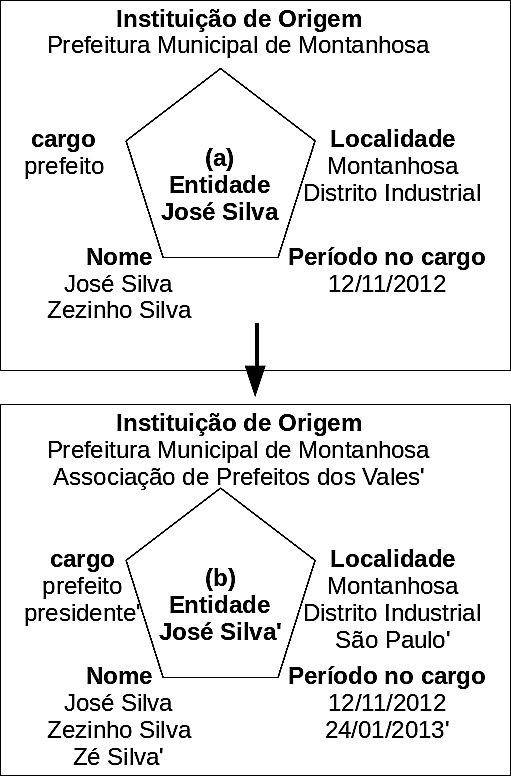
\includegraphics[width=.60\textwidth]{fig/facetasIndividuo.jpg}

	\legend{Fonte: elaborada pelo autor}
\end{figure}

%\textbf{Exemplo didático da ata.}
Um exemplo para o relacionamento entre entidades, facetas e termos, pode ser ilustrado por meio de uma ata de reunião, um típico documento de registro em instituições. O evento reunião teria acontecido em uma data, em um município e com participantes reconhecidos por nomes completos e suas respectivas instituições de origem. Um indivíduo denominado ``José Silva'' é uma entidade presente no documento, ilustrada na figura \ref{fig:facetasIndividuo} como um pentágono. Sua instituição de origem é a ``Prefeitura Municipal de Montanhosa'', onde está no cargo de ``prefeito''. \texttt{Nome}, \texttt{Instituição de origem}, \texttt{Cargo} e \texttt{Localidade} são facetas importantes para as entidades relacionadas a pessoas; e os termos ``José Silva'', ``Prefeitura Municipal de Montanhosa'' e ``prefeito'' estão associados às facetas na própria construção do texto da ata. O termo ``Montanhosa'' estaria associado à \texttt{Localidade} por dedução a partir da sua instituição de origem ou da localidade onde ocorreu a reunião. Facetas (em negrito) e seus respectivos termos constituem diferentes dimensões do pentágono (a) da figura \ref{fig:facetasIndividuo}.

%\textbf{Motivação para o reconhecimento das facetas comuns.}
Reconhecer esse conjunto de facetas comuns a maioria dos documentos é essencial para a organização automática da informação corporativa e para a interoperabilidade entre diferentes repositórios. Partindo do mesmo exemplo anterior, ao ser incluída uma nova faceta temporal \texttt{Período no cargo}, mesmo a data de início não tendo sido descrita na ata, sabe-se que na data da reunião ``José Silva'' era o prefeito em exercício. Assim, a \texttt{data de ocorrência} associada à reunião pode ser tomada como início do cargo de todas as entidades citadas no documento, inclusive da entidade ``José Silva''.

%\textbf{Associação dinâmica entre facetas e focos/termos.}
Essa associação entre localidades, datas, processos e entidades deve ser dinâmica e depende do reconhecimento de características espaciais, temporais, descritivas e lógicas. Nesse exemplo, a associação entre \texttt{data de ocorrência} da reunião e \texttt{período no cargo} de ``José Silva'' não é definitiva e vigora até que um novo documento evidencie uma data diferente para esta faceta, como é demonstrado na figura \ref{fig:facetasIndividuo}, em (b). Um documento de uma nova reunião ocorrida em São Paulo teria produzido as mudanças refletidas na entidade da figura \ref{fig:facetasIndividuo} (b), onde uma nova possibilidade de nome ocorre, a presidência de uma associação é registrada e o cargo de prefeito continua vigorando. A importância que esses novos termos assumem para cada faceta depende de muitas variáveis, como tempo, espaço, atores sociais envolvidos, a frequência e o uso dos novos e antigos termos nas mensagens que os documentos portam.

%\textbf{Possibilidades para outros modelos de interação, como o ranking e a visualização.}
A organização facetada da informação também torna mais flexíveis o \textit{ranking} e a visualização de resultados de busca. Na perspectiva de um usuário de informação, uma busca textual por ``negócios em montanhosa'' poderia muito bem retornar documentos de projetos em que ``José Silva'' seja citado mesmo que os termos ``Montanhosa'' ou ``Prefeitura Municipal de Montanhosa'' não estejam presentes. Adicionalmente, a própria desambiguação do termo montanhosa, uma cidade onde a organização possui unidade ou um adjetivo que pode pertencer a muitas entidades na coleção, é uma atividade necessária dentro do sistema de recuperação. Esse tipo de inferência espacial seria naturalmente realizado por um classificador humano experiente. Para uma busca ``negócios com prefeitura de montanhosa'', também seria natural que projetos recentes e antigos fossem recuperados, desde que incluam os nomes de ``José Silva'' ou de antigos prefeitos de Montanhosa, mesmo que os termos ``Prefeitura Municipal de Montanhosa'', ``prefeito'' ou ``Montanhosa'' não estejam explicitamente presentes no conteúdo do documento. Um buscador experiente poderia expandir a expressão de busca e incluir o nome dos vários prefeitos. Porém, uma organização de informação que inclua facetas espaciais, temporais, descritivas e lógicas também poderia subsidiar esses tipos de inferência, mas com a vantagem de considerar a temporalidade da informação, dos documentos e de cada prefeito-entidade indexado. Ou seja, não bastaria o modelo ser facetado para suportar buscas e recuperação de informação eficientes; o modelo precisa de facetas e tratamentos que realmente ajudem a evidenciar o contexto de entidades e documentos ao longo de todo seu ciclo de vida.






%\textbf{Visão facetada do usuário.}
Uma motivação tecnológica refere-se à visão facetada do usuário. Uma visão do esforço de busca do usuário informacional é a de que, ao invés de fornecer termos de interesse, o usuário normalmente fornece facetas de interesse. Por essa visão, caso o usuário de informação forneça um termo para espaço geográfico, como \emph{São Paulo}, seu interesse ultrapassa a existência do termo ou de uma notação para São Paulo, acrescentando à busca uma possibilidade de explorar a geografia do seu assunto de interesse. Na existência de um número como 1930 dado pelo usuário, se tem possivelmente uma faceta temporal pela qual a busca pode ser contextualizada e para qual até mesmo a terminologia do sistema de classificação precisa se adequar \cite{hong06,borges07,mir2ed}. Como exemplificado na seção anterior, se 1930 é um ano e São Paulo uma cidade ou estado, um documento com conteúdo que inclua \emph{adestramento} e \emph{mão de obra} refere-se provavelmente à capacitação dos funcionários das indústrias, o que requer um mapeamento de significado entre dois sistemas de classificação muito diferentes. 

%\textbf{Diversidade e tamanho do conjunto de documentos impõem dificuldades.}
Se explicar a intenção da busca em poucas palavras já parece difícil, mais difícil é a mesma intenção para espaços geográficos e janelas de tempo muito diferentes do espaço e do tempo da maioria dos documentos da coleção; e ainda mais difícil quando um componente de \textit{software} é o responsável por indexar e ``interpretar'' a necessidade de busca a partir de ideias e conceitos, recuperar documentos que possuem pouco mais que palavras e apresentar os resultados para o usuário de informação \cite{hong06}.

%\textbf{Diversidade e tamanho do conjunto de documentos são ampliados quando o contexto é a Web.}
A dificuldade é ainda maior no contexto de um sistema de recuperação de informação para documentos da \textit{World Wide Web} (WWW), ou um sistema de recuperação de informação de Internet. Na Internet estão documentos que versam sobre os assuntos mais diversos, em linguagem natural, sem metadados, nos mais diversos idiomas e linguagens especializadas \cite{hong06}. Neste caso, o sistema de classificação deve atender aos seguintes requisitos: 

\begin{citacao}
encontrar similaridade sem apenas encontrar padrões sem contexto; ser preciso e altamente descritivo; ser fácil de adicionar, apagar e atualizar classes e vocabulário sem a necessidade de reclassificar; deve suportar documentos digitais com uma informação que se expande continuamente \cite[p. 46, tradução nossa]{hong06}.
\end{citacao}

%\textbf{Web semântica e dados ligados como estratégias de enfrentamento tecnológico para a diversidade.}
Para grupos específicos de documentos na Internet, ou para comunidades específicas de usuários, existe perspectiva de que as tecnologias de Web semântica e de dados ligados (\textit{Linked data}) farão maravilhas. Boa parte de seus trabalhos são baseados em metadados construídos voluntariamente por usuários, sem um compromisso adequado com o controle terminológico para a manutenção de longo prazo dos repositórios. 

%\textbf{Facetas como recursos da navegação.}
Facetas, ou os atributos que são chamados de facetas, normalmente servem principalmente ao propósito de navegar parte desses grandes repositórios \cite{oren06facetedRDF}. O reconhecimento de facetas facilita também a navegação nos resultados uma vez que há um refinamento possível para cada faceta, algo não facilmente alcançável em um sistema de recuperação de informação baseado em palavras do texto completo \cite{sacco2006,auer09linkedgeodata,docubrowse10,maculan2011,pontesLima2012}. Porém, ``sem um compromisso com vocabulários controlados, resta pouca esperança de que as tecnologias da Web semântica alcancem seu fim'' \cite[p. 269, tradução nossa]{labarre2010}, principalmente fora do escopo das coleções de documentos altamente estruturados como é o caso de bibliotecas de teses e dissertações, de patentes e de bancos de dados.

%\textbf{Classificação facetada. Vantagens para documentos muito heterogêneos.}
\citeonline[p. 47]{hong06} defende o uso de classificação facetada em sistemas de recuperação de informação muito heterogêneos:

\begin{citacao}[english]
faceted classification focuses on the essential and constant characteristics/facets, which is useful for micro-grained rapidly changing information repository. It can be used to create deeper and more complex knowledge structures by exploring variants of combination \cite[p. 47]{hong06}.
\end{citacao} 

%\textbf{Vantagens para a consulta.}
A simplicidade dessa estrutura favorece os sistemas de recuperação de informação em que usuários devem buscar informação sobre entidades, espaços e tempos conhecidos \cite{toda08,entityCentric12}, especialmente no momento da consulta \cite{andrade06}. Este é o caso principalmente do contexto dos sistemas de recuperação de informação geográficos, em que espaço e tempo, duas facetas importantes em quase todo sistema de informação, são bem melhor estruturados e onde estão presentes alguns métodos de ordenação espaço-temporal.

%\textbf{Vantagens para a ordenação.}
Como exemplo, \citeonline{ehlen09} e \citeonline{toda08} descrevem aplicações para a ordenação baseada em múltiplas facetas, como a localização de documentos que pertençam à região de interesse do usuário, sendo que a relevância da faceta espacial é dada pela menor distância do ponto onde o usuário se encontra, o que é particularmente útil em serviços de localização e serviços móveis. A faceta temporal também é considerada em muitas aplicações em que novidades sobre um certo fenômeno, ao invés de relatos históricos, são preferíveis. É o caso de repositórios de notícias, serviços de monitoramento de catástrofe ou de trânsito. De fato, o interesse é por um método que consiga mensurar a importância do contexto geográfico, temporal ou temático em tempo de consulta \cite{andrade06} e responda com eficiência ao usuário de informação \cite{yuCai07,GarciaCumbreras09}.

%\textbf{Vantagens para a manutenção.}
Uma motivação metodológica refere-se à flexibilidade da classificação facetada. Como a classificação facetada é flexível e, portanto, adequada para modelar domínios em contínua expansão e mudança, mesmo os sistemas de classificação inicialmente implementados sem um sólido embasamento teórico podem ser beneficiados \cite{hong06,labarre2010}. Ou, em outras palavras, independentemente da qualidade da abordagem implementada pelos sistemas de recuperação de informação que se encontram na literatura, a teoria da análise facetada posta em prática no contexto desses sistemas e esses sistemas postos em avaliação sob a lente da teoria da análise facetada constitui um passo importante para a área.







%\textbf{Link para próxima seção.}
Na próxima seção são investigadas as principais pesquisas sobre avaliação de modelos de domínio e sobre avaliação de sistemas  de recuperação de informação, do desempenho dos processos de indexação e da recuperação de informação.


\section{Avaliação de sistemas de recuperação de informação}

%\textbf{Introdução.}
Como a análise de domínio deve produzir um produto, um modelo de alto nível do domínio em estudo, após validado ele precisa ter sua utilidade avaliada. Também há muita diversidade de métricas de avaliação de utilidade desse tipo de instrumento, sendo que diferentes métricas refletem os objetivos do modelo, exatamente como acontece com a escolha dos métodos que são executados no processo de análise de domínio. Como o modelo resultante desta tese objetiva favorecer a atividade de recuperação de informação, sua avaliação se dá indiretamente, pela avaliação do desempenho da própria recuperação de informação.

%\textbf{Coleções de referência.}
A presença de uma coleção de referência favorece a comparação de sistemas de recuperação de informação e a definição de valores que sirvam como base de comparação. O contrário, quando experimentos são realizados em coleções privadas, a publicação de resultados se baseia muitas vezes em informação protegida, não disponível publicamente e muitas vezes sensível. Há muitas metodologias de avaliação de sistemas de recuperação de informação \cite{irEvaluation02,evaluationWithIncompleteInformation04,bucher05,sakai08ret,DBLP:conf/clef/2008}, algumas delas bem aceitas na indústria e na academia. Porém, há limitações para avaliação de sistemas corporativos pelas mesmas metodologias, dadas suas especificidades \cite{craswell05}.

%\textbf{Coleção de referência Enterprise e as limitações para se constituir uma coleção.}
Embora a trilha \textit{Enterprise} da \textit{Text Retrieval Conference} ofereça uma coleção de referência para sanar parte das limitações de avaliação; ao ser baseada apenas em documentos da \textit{Web} pública de uma empresa ela também se mostra insuficiente para avaliar a busca por recursos de informação reais \cite{bailey07}. Porém, a dificuldade de melhorar o \textit{corpus} de avaliação está na dificuldade de expor dados sensíveis de uma empresa, seus clientes, funcionários, fornecedores e suas estratégias de negócio. Mesmo uma empresa pública ou governo conta com informação sensível, protegida por lei, não sendo necessariamente um bom candidato a fornecedor de dados de avaliação. Por essa razão, muito do esforço de atingir os objetivos da trilha \textit{Enterprise}, que aconteceu até o ano de 2008, foi transferida para uma nova trilha, \textit{Entity Search} (ou, Busca por Entidades), que aconteceu até o ano de 2011, vislumbrando reconhecer entidades humanas e não-humanas e em diferentes escalas, das intranets de empresa à toda a Web \cite{balog08}.

%\textbf{Avaliação em Fóruns de avaliação.}
As técnicas e sistemas implementados têm sido confrontados com outros sistemas sob o mesmo prisma de avaliação, onde são encontradas várias metodologias. No entanto, os diferentes prismas e metodologias normalmente valorizam mais algumas fontes de evidências do que outros. É o caso da trilha \textit{GeoCLEF}, do \textit{Cross-Language Evaluation Forum} (CLEF), constituindo um \textit{framework} através do qual sistemas que utilizem linguagens europeias podem ser comparados sob os mesmos critérios e com a mesma massa de dados \cite{domenech07,cardoso08,anastacio09}, visando reconhecer evidências espaciais e linguísticas. Metodologia similar, porém específica para sistemas em língua portuguesa, é denominada Avaliação de Reconhecimento de Entidades Mencionadas (HAREM) \cite{harem07}.

%\textbf{Avaliação através de Usuários de sistemas de recuperação de informação.}
Outra estratégia de avaliação baseia-se na adoção direta dos usuários do sistema de recuperação de informação. É o caso do \textit{Open Directory Project} (ODP), onde são realizadas as mesmas atividades de avaliação e os resultados são comparados com aqueles anotados manualmente por voluntários \cite{amitay04}, e as metodologias de avaliação que empregam os próprios usuários do sistema como forma de avaliação mais criteriosa dos componentes de consulta e da qualidade percebida da resposta \cite{bucher05,yuCai07,pontes13}. Em todas as metodologias de avaliação são adotadas métricas muito próximas daquelas adotadas para sistemas convencionais, sendo que alguns trabalhos sugerem a necessidade de estabelecer metodologias mais adequadas para alguns tipos específicos de fontes de evidência e de coleções \cite{domenech07,sakai08ret}.

%\textbf{Motivação para adotar duas coleções.}
Um fórum que imponha o reconhecimento automático de diversos tipos de evidência, como espacial, temporal, social, linguístico e temático, por exemplo, não está disponível atualmente. Sua ausência, apesar de dificultar a tarefa de avaliação de sistemas de recuperação de informação, não representa o maior desafio de avaliação. O maior desafio continua a ser definir critérios formais de relevância, coleções de referência e métricas empíricas de desempenho adequados para diferentes atores sociais e contextos de uso. Por essa razão, esta pesquisa adota os resultados de \citeonline{bailey07} e \citeonline{balog08} como base de comparação, mas não pode dispensar uma avaliação complementar, com coleção privada e usuários reais, para garantir que os resultados realmente representem soluções de recuperação para situações mais próximas da realidade corporativa.

%\textbf{A base metodológica para avaliação e as diferenças associadas.}
Os procedimentos metodológicos para avaliação desta pesquisa sobre a coleção privada deve diferir pouco daqueles adotados por \citeonline{bailey07csiro}. A principal diferença é a perspectiva interpretativa adotada neste estudo; a importância dada à análise de domínio como componente formal da construção da coleção de referência e do modelo do domínio; o estabelecimento dos contextos de uso mais úteis para os usuários de informação; e o reconhecimento dos gêneros textuais e das linguagens adotadas por usuários e produtores de informação corporativa \cite{lykke2011domain}.




%\section{Indexação}

%?

%linguística

%temporal

%geográfica


%No entanto, entre os trabalhos encontrados, é senso comum que não há vantagem percebida em se usar técnicas geográficas ao invés das abordagens convencionais sobre o contexto geoespacial \citep{anastacio09,cardosoSantos08}, o que denota que muitos aperfeiçoamentos são ainda necessários em RIG. Identificados e descritos brevemente os principais trabalhos da área, é detalhado a seguir o projeto de pesquisa.





%Considerações finais e trabalhos futuros

%Esse capítulo empreendeu uma revisão de literatura sobre análise de domínio e organização da informação, comparando criticamente as abordagens intelectuais e automática que favorecem a classificação e indexação automáticas de coleções, usando ambientes corporativos como pano de fundo.












%O acervo de informação, principalmente digital, de pessoas e empresas tem crescido significativamente pelas facilidades de produção, compartilhamento e armazenamento, este último parecendo quase não ocupar espaço físico pelos avanços tecnológicos.

%No entanto, com esse crescimento, problemas associados à recuperação de informação têm surgido, sendo particularmente mais sérios quando a recuperação de informação é tarefa essencial para realizar trabalho e tomar decisões, algo que acontece em diversas áreas assim como em empresas.

%São diversas as iniciativas que tentam minimizar os problemas de RI, especialmente da informação digital, mas iniciativas são mais efetivas quando baseadas em uma organização da informação adequada e compatível com a forma pela qual ocorre a organização do conhecimento.

%Adicionalmente, com o ritmo acelerado da produção de informação, diversos desafios se impõem à classificação e indexação da informação por esforço intelectual, exigindo muitas vezes técnicas automáticas ou semiautomáticas de classificação e indexação com precisão e controle de erros altos. Por outro lado, o próprio desenvolvimento do conhecimento humano, a evolução das áreas de conhecimento e da linguagem.... criam obstáculos sérios para a eficiência destas técnicas automáticas, na convergência de esforços das ciências da informação, da computação, da linguística, da ciência cognitiva e outras.

%Incluir justificativa para facetadas.

%O estado da arte e da técnica da organização da informação visando a recuperação da informação, da informação digital especialmente, é a principal questão deste capítulo.

%Além de objetivar mapear os principais trabalhos em organização da informação, este capítulo também se propõe a encontrar técnicas que favoreçam a classificação e indexação automáticas de coleções digitais, especialmente de documentos corporativos.

%A organização organiza-se em X seções. Na primeira são tratadas as bases teóricas de classificação de informação, inclusive da organização multifacetada da informação. Na segunda, são apresentadas referências para técnicas de desambiguação e de indexação de tema, tempo e espaço, .... Finalmente, na terceira seção são discutidas as principais metodologias de avaliação da recuperação de informação.
%bases teóricas de classificação
%desambiguação de nomes de pessoas
%desambiguação de nomes de empresas
%desambiguação de sentido de palavras
%desambiguação de tempo
%desambiguação de espaço
%indexação de pessoas
%indexação de empresas
%indexação de assunto (assunto? tema? termos?)
%indexação de tempo
%indexação de espaço
%metodologias de avaliação
%fóruns de avaliação


%\section{Classificação de Informação}
%Classificação

%\section{Desambiguação e Indexação}
%Desambiguação e Indexação

%\section{Avaliação de Recuperação de Informação}
%\label{avaliacao}

%Avaliação de Recuperação de Informação


%In despite of all these, regretfully, we still tend to put all bets on technology every time new technology appears. In answering the question of why it is so hard to find information on the Web, and why search engines aren't more helpful?, Rosenfeld replied that one reason for this confusion is that it's really hard to express our information needs in words, much less translate those words into a query language understood by a dumb piece of software (that is, search engines). Another reason is that it's really hard to index the ideas and concepts that are stored in text in a way that this dumb software can understand (and therefore find). So when we do a search, we're asking something much dumber than we are to do something we find hard to do ourselves'' [Morville, 2002]

%\citep{hong06}

%As formas pelas quais as pessoas buscam na Web e na empresa tendem a ser semelhantes. Por isso, muitos dos problemas percebidos pelos usuários e relacionados à consulta e ao \textit{ranking} são comuns.









%Definições
%Indexação
%Indexação é o processo intelectual que envolve atividades cognitivas na compreensão do texto e a composição da representação do documento. E, por ser uma atividade intelectual, pode se beneficiar particularmente de teorias e métodos da Psicologia Cognitiva e da Teoria de Soluções de Problemas (David et alii, 1995, p.49). Wellish (1995)**, citado por Jacob & Shaw (1998, p.159), descreve indexação como o ato de indicar ou apontar o conteúdo intelectual de uma coleção. Esta definição mascara a natureza cognitiva do processo de indexação, por enfatizar o produto físico do processo, e não a análise de conteúdo.
%Conceito
%
%Termo
%



%A principal metodologia de projeto e implementação de um sistema de recuperação de informação geográfica (RIG) baseia-se em um sistema de RI convencional, com os mesmos componentes, onde são implementadas as técnicas de tratamento da informação geográfica \cite{anastacio09, cardosoSantos08}. Com isso, os componentes incluem os métodos de coleta de documentos, de reconhecimento de entidades ou \textit{geoparsing} e de identificação e desambiguação dessas entidades ou geocodificação. A tarefa de indexação, do conteúdo e das referências geográficas reconhecidas, também faz-se necessária para manter o sistema em condições de fornecer respostas precisas e eficientes, enquanto que a interface com o usuário e o componente de classificação e ordenação desempenham papel importante para atender seu usuário.



%\section{Recuperação de informação corporativa}

%Enterprise Information Retrieval

%Principais diferenças. Cabe aqui ou ao longo da revisão de literatura?

%Estudos sobre o custo de tempo necessário para realizar pesquisas na empresa

%Pesquisa como parte de tarefas próprias da rotina empresarial. Exemplos de tarefas.

%A eficiência para o usuário de um sistema de recuperação de informação se reflete em custos menores para a organização, no contexto de EIR, que garante continuidade de negócios, escalabilidade, privacidade.

%Arquitetura de um SRI corporativa. Cada componente da arquitetura refere-se a uma fase a ser apresentada a seguir.








%\section{Coleta}

%Crawler

%Fontes internas e externas.

%Preservação do documento original apresenta riscos para segurança e nem sempre é possível.

%No caso de federação, nem sempre é possível ter acesso aos documentos. Só é possível encaminhar pesquisas e mesclar os resultados com o resultado final ao usuário.

%Quando há muitas réplicas do mesmo documento, um problema caro de resolver é exposto, com risco para segurança em caso de informação sensível ou dificuldades de armazenamento ou processamento para identificação da réplica.

%Aplicação de hash para controle de alteração. Versões do documento. Nova coleta do documento. Problemas das réplicas identicas ou levemente modificadas.



%Faltam detalhes do coletor/crawler

%Textos, imagens, sons, desenhos

%Diferentes formatos de arquivos e codificação de dados

%Presença de dados em arquivos, bancos de dados distribuídos em servidores e clientes por toda a empresa e fora dela

%Compactação, criptografia

%Acessibilidade limitada à informação por dificuldades de permissões, conectividade, baixa qualidade de metadados


%\section{Parsing e reconhecimento de entidades}


%Os documentos, materializados em arquivos, normalmente contam com metadados em seu formato original. Porém, tais metadados não estão sempre disponíveis. Frequentemente são imprecisos, estáticos e desatualizados.

%Especialmente em um contexto de pesquisa multifacetada, o reconhecimento de entidades assume particular importância para a eficiência do SRI como um todo, e para a organização da informação, em particular.

%Processar o máximo de texto dos documentos, porém nem todo documento tem seu texto disponível para processamento.

%Documentos podem estar compactados, criptografados, protegidos contra extração de texto, codificados em formato proprietário, corrompidos, etc.

%Outra classe de problema trata do reconhecimento de entidades/facetas por padrão de texto, proximidade de um termo em relação a outros, localização no documento (início, meio, fim) e através de outras fontes de evidência para adequada desambiguação e correta indexação.







%\section{Indexação}

%Indexar o máximo de fontes de evidência de relevância leva a aumentar o número de facetas sobre as quais documentos e informação são classificados.

%Algumas fontes de evidência podem ser:
%local físico
%geográfico
%tipo de arquivo/formato
%nome do arquivo
%tipo do documento e outras informações mais.

%Também são úteis metadados do administrador, do usuário, texto completo, data de produção, volumes de réplicas, referências a nomes de entidades/facetas, idioma, cliques sobre o documento ou frequência de uso do documento pelo grupo, pelo usuário, pela empresa.

%Os principais problemas são: como tratar a diversidade de tipos, a ausência de atributos de alguns com a presença de outros, o custo da estrutura de dados e do acesso a tantas facetas, a importância dos arquivos sobre outros para os quais não há permissão de acesso, como indexar sem que a recomposição de arquivos sensíveis seja possível, como identificar réplicas e versões com menor custo, a identificação do idioma e como priorizar idiomas, como indexar múltiplos idiomas, qual estrutura adotar para cada faceta, como indexar perfis de usuários e se é necessário. Como um perfil de usuário pode parametrizar interesse ou prioridade de umas facetas sobre outras.

%Atualização de índice

%Múltiplas facetas requerem estrutura ou estruturas próprias?

%Um índice por faceta? Ou um para todo o conjunto?

%Um índice por repositório ou um índice para todo o conjunto?



%\section{Consulta}

%A forma através da qual o usuário interage com o sistema pode impactar na qualidade dos resultados e do sistema como um todo. Para isso, um componente essencial é a interface de consulta, onde o usuário fornece seus interesses, temáticos ou espaciais. Nesse local, duas abordagens possíveis são a separação da entrada de tema e espaço \citep{yuCai07} ou a reunião de ambos no mesmo ponto de entrada, sendo necessários o \textit{geoparsing} e a geocodificação, assim como ocorrem no conteúdo dos documentos, também no texto da entrada. Trabalhos relacionados a identificação geoespacial na consulta têm sido realizados também por \citet{gan08}.

%influência da IU na experiência e satisfação do usuário.

%Identificação de termos e facetas de interesse do usuário. Atributos do usuário como quem, onde, quando, como, porquê.

%Como fazer um parsing adequado para cada usuário.

%Busca dinâmica facetada \citep{pontesLima2012}.

%Como os resultados devem ser visualizados? Colunas, ícones, visualizações. Não é bem para consulta ou consulta interativa, mas está dentro de IU.

%Consulta em contexto: local, momento, quem, porquê, como, ...

%Qual o conjunto de repositórios mais relevante para o usuário naquele contexto de busca? Este problema se junta ao processamento da consulta.

%\section{Processamento de consulta}

%Qual o conjunto de repositórios mais relevante para o usuário naquele contexto de busca? Este problema se junta ao processamento da consulta.

%Federação ou centralização de metadados.

%Segurança do sistema e dos dados. Acesso remoto. Acesso interno.

%Estatísticas e logs de acesso. Eficiência computacional para acesso às estruturas de dados, localização de termos, seleção e ordenação de registros.

%Processamento distribuído

%Controle de acesso - segurança - direito

%Information Filtering

%Profiles




%A forma através da qual o usuário interage com o sistema pode impactar na qualidade dos resultados e do sistema como um todo. Para isso, um componente essencial é a interface de consulta, onde o usuário fornece seus interesses, temáticos ou espaciais. Nesse local, duas abordagens possíveis são a separação da entrada de tema e espaço \citep{yuCai07} ou a reunião de ambos no mesmo ponto de entrada, sendo necessários o \textit{geoparsing} e a geocodificação, assim como ocorrem no conteúdo dos documentos, também no texto da entrada. Trabalhos relacionados a identificação geoespacial na consulta têm sido realizados também por \citet{gan08}.



%\section{Ranking ou Ordenação}

%problemas com TFIDF

%\citep{akritidis11} para ranking


%Quais propostas existem?

%Colunas para diferentes tipos de dados, com ranking diferente

%Combinação de rankings

%Pesos

%Criação de profiles

%A partir do reconhecimento de facetas, o ranking pode ser adaptativo?

%Ranking de relevância a partir de facetas organizadas em estruturas de dados diferentes, ao invés de métricas baseadas na frequência da ocorrência de termos.

%Outro problema relevante é a ordenação ou \textit{ranking} de documentos para a construção da resposta ao usuário. Na área de RIG, dada uma entrada do usuário, é necessário ordenar os documentos que eventualmente atendam ao seu interesse, combinando as variáveis temáticas e espaciais. Porém, tal ordenação mostra-se complexa uma vez que é difícil assinalar qual faceta é a mais importante ao usuário, se o tema de interesse ou a região de interesse. É provável que por este problema os sistemas geográficos ainda não apresentem ganhos significativos de precisão nas consultas se comparados aos sistemas convencionais.

%A maioria dos trabalhos projeta um sistema que usa dois índices para o \textit{ranking} do resultado de consulta, um baseado na relevância do texto ou conteúdo do documento e outro baseado no contexto espacial, havendo diferenças substanciais na parte geográfica entre os trabalhos. A própria tarefa de indexação de cada documento normalmente é realizada em separado, sendo que cada documento é georreferenciado e alocado no espaço de coordenadas geográficas ao mesmo tempo em que é indexado por seus termos no espaço vetorial \citep{yuCai07}. 

%\Citet{li06} implementam a ordenação geográfica por meio de uma matriz pela qual a superfície da Terra é dividida. \citet{martins10} usam métodos de aprendizado de máquina para a criação do \textit{ranking} temático e geográfico em uma única função de ordenação por relevância, baseada na estratégia \textit{Learning to Rank}. \citet{ehlen09} e \citet{toda08} focam outras aplicações para a ordenação, como a localização de documentos que pertençam à região de interesse do usuário, sendo que a relevância do espaço geográfico é dada pela menor distância do ponto onde o usuário se encontra, o que é particularmente útil em serviços de localização e serviços móveis. De fato, o interesse é por um método que consiga mensurar a importância do contexto geográfico ou temático em tempo de consulta \citep{andrade06} e responda com eficiência ao usuário \citep{GarciaCumbreras09, yuCai07}.





%\section{Atualização da coleção}

%Arquivos são atualizados e sua relevância pode mudar em função de tais atualizações.

%Eficiência da coleta de arquivos para verificação de atualização.

%Da reindexação de arquivos atualizados. Da exclusão de arquivos do índice. Da inclusão de novos arquivos. Eficiência tanto para armazenamento quanto para processamento de indexação, de consultas e de verificação de alteração.








%Métricas?

%EIR contam com repositório de avaliação? TREC?

%Quais outras propostas existem para avaliação? Como discutem a eficiência delas?








%\section{Recuperação de informação multifacetada}

%O título está ok?

%Quais facetas exemplificar?

%Em um SRI geral, para Web, e Enterprise?

%Os sistemas tendem a ser estatísticos, algo que provoca insatisfação ao usuário.

%Um passo adiante é necessário para aumentar a satisfação do usuário, pelo melhoria de métricas comuns como precisão e revocação, mas também pela redução do custo de tempo para o uso de SRI, algo particularmente útil no contexto de EIR.

%Custo de tempo não significa um sistema simplesmente mais rápido, mas um processo de busca por informação que encerra no menor tempo possível, entre seu início e a localização de toda a informação necessária para se realizar uma tarefa.

%Quais atributos podem ser usados da coleta para ajudar no reconhecimento de facetas? E no parsing? E como o índice deve ser implementado?

%Quais alterações devem ser realizadas na busca (IU)? Quais as implicações deste modelo para o processamento? E para a atualização?

%docubrowse \cite{docubrowse10}







%
%\chapter{Análise de domínio corporativo}
%\label{analiseDominio}
%%\chapter{Uma análise de domínio corporativo} - manter comentado

	\begin{flushright}
		\textit{``Não se possui o que não se compreende''.
		\\Johann Goethe}
	\end{flushright}


%Problema
%\textbf{Problema do capítulo: encontrar características do domínio corporativo.}
Este capítulo trata da caracterização do domínio corporativo e objetiva explicitar quais características da informação corporativa são comuns a diferentes instituições. Dessa forma, o capítulo apresenta uma proposta de generalização do domínio corporativo e ilustra algumas características descobertas a partir da análise de domínio utilizando as técnicas de análise de assunto e análise facetada, empreendidas em cada uma das coleções de documentos pesquisadas. Dentro do domínio corporativo, somente através de uma análise de domínio rigorosa pode-se tentar responder se as facetas adotadas por empresas diferentes apresentam alguma semelhança.


%Objetivo Geral
%O objetivo deste capítulo é determinar um conjunto mínimo de facetas para entidades corporativas que permita sua representação com um equilíbrio entre a expressividade de contexto e baixo custo computacional de reconhecimento e indexação de entidades corporativas por meio de métodos automáticos.

%São objetivos específicos a identificação das facetas que sejam comuns ao domínio corporativo; e também a identificação das características mais específicas que precisem ser estudadas e tratadas com atenção ao contexto e às necessidades de cada empresa, sob risco de não atender aos objetivos de recuperação de informação de seus respectivos usuários informacionais.

%Motivação/Justificativa

%Para o projeto de um sistema de recuperação de informação, muitas vezes é necessário ter contato com a coleção de documentos e necessidades de usuários. Para sistemas mais caros, é comum tentar generalizar seus usos dentro de um domínio para que o sistema seja distribuído com o menor custo. Do ponto de vista científico, a tentativa de generalização é uma curiosidade científica importante para garantir a evolução dos sistemas documentários, em geral, e de um domínio em particular.

%No entanto, toda e qualquer tentativa de generalização no domínio corporativo deve permanentemente enfrentar dificuldades de acesso a amostras de informação corporativa.




%Procedimento metodológico

%\textbf{Procedimentos metodológicos da análise de domínio.}
Os procedimentos metodológicos da análise de domínio foram executados como segue: i-a) análise de assuntos e o levantamento de termos mais significativos em cada uma das coleções de documentos; i-b) formação de assuntos pela leitura e pela aplicação das técnicas de dissecação e desnudação; ii) categorização dos assuntos pela aplicação da técnica da análise facetada em cada coleção de documentos; e iii) consolidação das categorias, facetas e subfacetas comuns às duas coleções de documentos.

%\textbf{Sumário para procedimentos metodológicos indicando suas respectivas seções e colocando os subprodutos nos anexos.}
Os procedimentos de análise, formação e categorização de assuntos (i-a, i-b e ii, respectivamente) foram executados em cada coleção, isoladamente, pelo autor deste trabalho. Os dois primeiros são reportados na seção \ref{analiseFormacaoDeAssuntos} e a categorização é reportada na seção \ref{categorizacao}. Todos os assuntos devidamente categorizados estão disponíveis nos anexos \ref{anexoassuntosCEFETMGdocs}, \ref{anexoassuntosCSIROqueries} e \ref{anexoassuntosCSIROdocs}.

%\textbf{Sumário para o produto preliminar da análise de domínio corporativo.}
Por último, a análise preliminar do domínio corporativo é encerrada pelo procedimento de consolidação das facetas comuns às coleções e de avaliação do grau de similaridade que tais facetas supostamente apresentam no domínio. Seus resultados são apresentados e discutidos na seção \ref{analiseDominioRes}.


\section{Análise de assuntos e formação de assuntos}
\label{analiseFormacaoDeAssuntos}

%\textbf{Propósito da análise de assuntos.}\footnote{Inverti os parágrafos, como pediu.}
A análise de assuntos constitui a análise intelectual dos documentos de cada coleção com o propósito de interpretá-los e de representar seus assuntos por meio de termos em linguagem natural. Em seguida, sobre os assuntos resultantes foram aplicadas as técnicas de dissecação e desnudação para formação de assuntos adicionais. O processamento da análise e formação de assuntos foi dividido em três fases e ocorreu linearmente sobre as coleções particular e pública, nessa ordem.

%\textbf{Análise de assuntos sobre as duas coleções.}\footnote{Você pediu para eu colocar algo como ``Primeiramente foi analisada a coleção particular seguindo as propostas: leitura..., análise dos documentos, seleção dos termos representativos, ...''. Porém, observe que essas operações já estão no segundo parágrafo deste capítulo. Por que coloquei assim? Porque são 3 amostras de 2 coleções. Os mesmos procedimentos metodológicos de análise são aplicados nas 3 amostras. Logo, ao invés de repetir antes de cada amostra, eu falo uma vez só no início do capítulo. Ok? Eu melhorei a descrição dos procedimentos, adicionando mais detalhes da formação de assuntos, como pediu.}
A análise de assuntos foi realizada sobre duas coleções de documentos provenientes de duas empresas, o Centro Federal de Educação Tecnológica de Minas Gerais (CEFETMG) e a \textit{Commonwealth Scientific and Industrial Research Organisation} (CSIRO). Como as coleções pertencem a empresas diferentes, sua comparação dá-se pelos assuntos corporativos que ambas tratam. Isto é, dois assuntos, mesmo representados por termos distintos, podem ser considerados idênticos por uma avaliação intelectual do classificador. É o caso do assunto país, representado igualmente por Brasil ou \textit{Australia}; de instituição, representado por CEFETMG ou CSIRO; e de serviço, representado por Curso de graduação ou por \textit{Research}. Por outro lado, um mesmo termo pode referir-se a assuntos diferentes para cada empresa. Um exemplo é o termo \textit{site} que denota um \textit{Web site} ou um local de funcionamento da empresa para a CSIRO, enquanto só representa o primeiro assunto para a empresa CEFETMG. 


\subsection{Primeira fase de processamento: documentos da coleção particular}

%\textbf{Explicação sobre a coleção particular.}
A primeira fase de processamento da análise de assuntos ocorreu sobre a coleção particular de documentos que pertencem à empresa CEFETMG. A coleção particular foi produzida por um gerente da empresa como um conjunto significativo e útil de documentos para o trabalho rotineiro e para tomada de decisão. Esses documentos estavam organizados em repositórios, sendo possível encontrar réplicas de um documento em um ou mais repositórios. Os repositórios mobilizados constituem a principal fonte de informação que gerentes e usuários de informação têm usado na empresa entre os anos de 2012 e 2013; portanto essa coleção é mais eficaz que uma amostra aleatória do arquivo corrente para o propósito desta pesquisa. A tabela \ref{tab:documentosParticular} apresenta os repositórios a que pertencem os documentos com a quantidade de documentos e páginas oriundos de cada um.

% Booktabs require to add \usepackage{booktabs} to your document preamble
\begin{table}[h]
\caption{Composição da coleção particular}
\centering
\begin{tabular}{@{}lrrr@{}}
\toprule
                               & \multicolumn{1}{c}{\textbf{Documentos (D)}} & \multicolumn{1}{c}{\textbf{Páginas (P)}} & \multicolumn{1}{c}{\textbf{P/D}} \\ \midrule
Formulários                    & 9                                           & 11                                       & 1,2                              \\ %\midrule
Atas de Informática            & 11                                          & 28                                       & 2,5                              \\ %\midrule
Páginas Web                    & 5                                           & 5                                        & 1                                \\ %\midrule
Atas da Congregação            & 55                                          & 124                                      & 2,3                              \\ %\midrule
Atas do Fórum de Coordenadores & 14                                          & 45                                       & 3,2                              \\ %\midrule
Notícias externas              & 210                                         & 210                                      & 1                                \\ %\midrule
Notícias internas              & 384                                         & 384                                      & 1                                \\ %\midrule
Projetos                       & 4                                           & 426                                      & 106,5                            \\ %\midrule
Normas internas                & 6                                           & 107                                      & 17,8                             \\ %\midrule
Normas externas                & 1                                           & 109                                      & 109                              \\ %\midrule
Correspondências               & 606                                         & 606                                      & 1                                \\ \midrule
\textbf{Total}                 & \textbf{1305}                               & \textbf{2055}                            & \textbf{1,6}                     \\ \bottomrule
\end{tabular}
\label{tab:documentosParticular}
\legend{Fonte: Elaborada pelo autor.}
\end{table}

%Validação? Amostral? Kappa?

%\textbf{Levantamento dos assuntos.}
Um único profissional da área, autor desta tese, leu 1305 documentos produzidos entre os anos de 2007 e 2013 e anotou os assuntos presentes na medida em que foram identificados. Nessa etapa, os assuntos foram anotados através do termo em linguagem natural que melhor o representava, empregando a terminologia adotada pela instituição em pelo menos um documento da coleção. O documento onde o assunto/termo aparecia pela primeira vez também foi anotado, mas esse dado não é disponibilizado nesta tese por violar o acordo de sigilo. O objetivo é evitar constrangimentos por provável informação, e.g.: o termo Joseph ocorre pela primeira vez em um processo disciplinar.

\begin{figure}
	\caption{\label{fig:assuntosIdentificadosParticular}Novos assuntos descobertos em repositórios da coleção particular}

	\centering
		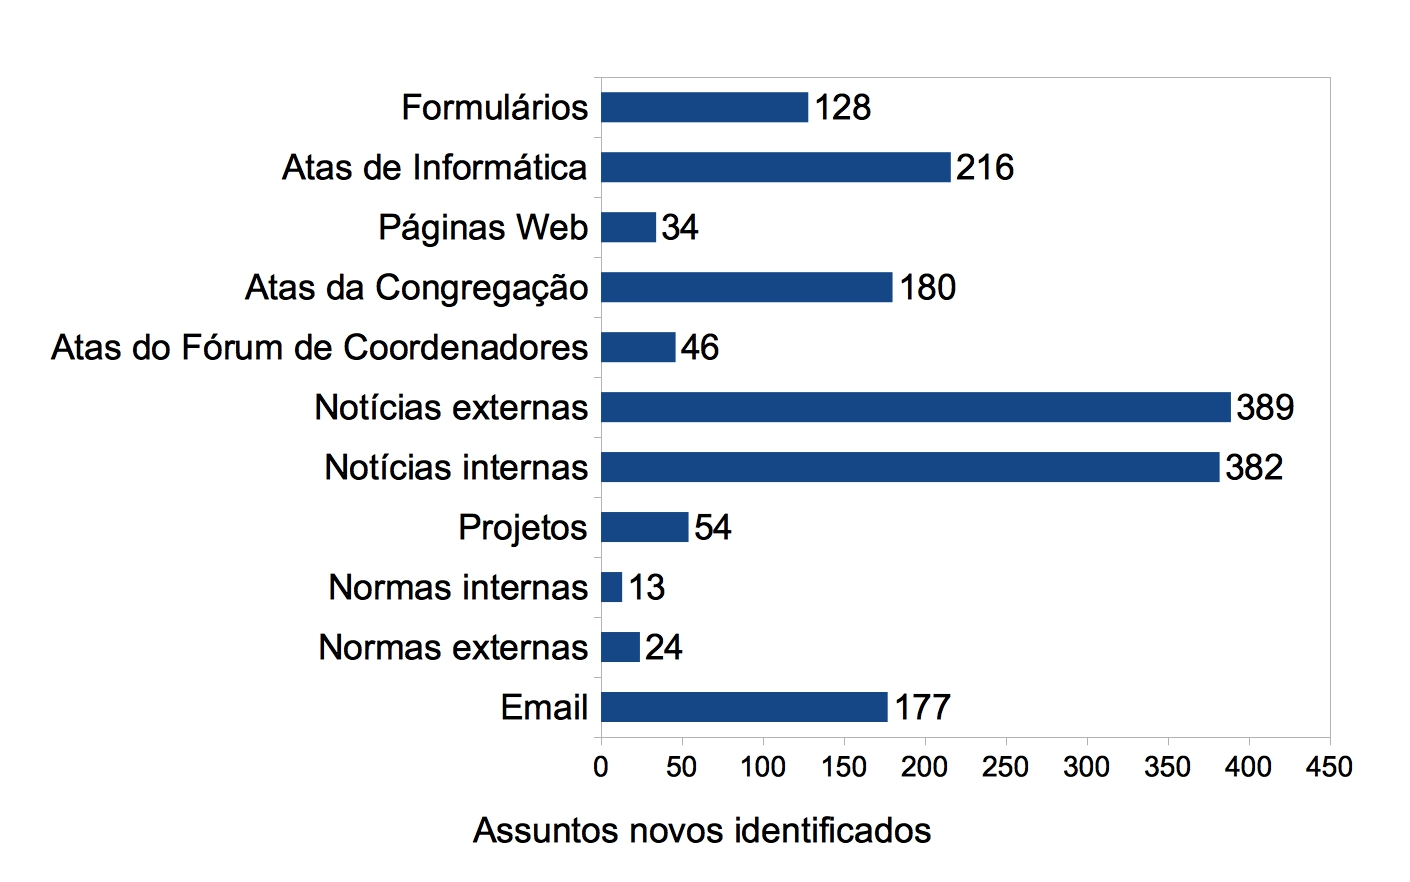
\includegraphics[width=1.0\textwidth]{fig/assuntosIdentificadosParticular.jpg}

	\legend{Fonte: elaborada pelo autor}
\end{figure}

%\textbf{Dissecação e desnudação aplicadas.}
Após a leitura de cada documento e a anotação dos novos assuntos descobertos, foram aplicados os métodos de dissecação e desnudação para formação de assuntos adicionais. 

Através do método de dissecação se divide o universo analisado em lâminas, sendo que cada lâmina representa um assunto básico ou um isolado. Por meio de um processo iterativo, as lâminas são dividas em novas lâminas de níveis diferentes. Um exemplo de formação de assuntos pela aplicação do método de dissecação é o renque Manhã, Noite e Tarde para turnos de trabalho. 

Através do método de desnudação são identificados assuntos com grande profundidade a partir de assuntos mais gerais ou isolados. O resultado é uma cadeia de assuntos em que a profundidade aumenta e a extensão diminui a cada iteração do método.
Um exemplo de formação de assuntos pelo método de desnudação, é a cadeia Ensino $\supset$ Ensino médio e profissional técnico de nível médio $\supset$ Ensino técnico.
Ou seja, Ensino técnico é subconjunto de Ensino médio e profissional técnico de nível médio, que está contido em Ensino.

Os demais três métodos de formação de assuntos, laminação, agregação e sobreposição, não foram utilizados na amostra, uma vez que foi usada a linguagem natural presente na amostra, inexistindo vocabulário controlado para controle terminológico.

%\textbf{Assuntos resultantes.}
A figura \ref{fig:assuntosIdentificadosParticular} mostra a ordem de processamento, do repositório de formulários ao repositório de Emails, e o número de novos assuntos descobertos em cada repositório da coleção particular. Porém, caso outra ordem de processamento fosse seguida o total de assuntos descobertos continuaria o mesmo. A análise e formação de assuntos na coleção particular consumiu o tempo total de 29 horas e 20 minutos e resultou em 1643 assuntos que estão listados no anexo \ref{anexoassuntosCEFETMGdocs}. 



\subsection{Segunda fase de processamento: queries e narrativas da coleção pública}

%\textbf{Explicação sobre a coleção pública.}
A segunda fase de processamento da análise de assuntos ocorreu sobre a coleção de referência pública usada na trilha \textit{Enterprise} da \textit{Text Retrieval Conference} (TREC) até o ano de 2008. Trata-se de uma coleção de 370715 páginas \textit{Web} públicas da empresa CSIRO; além de um conjunto de 77 narrativas e 77 \textit{queries} disponibilizadas por funcionários da CSIRO como as questões mais frequentemente respondidas por funcionários da CSIRO para clientes externos \cite{bailey07csiro}. Apenas as narrativas e \textit{queries} foram adotadas nesta segunda fase. As narrativas correspondem a uma questão de exemplo escrita por um cliente e enviada para funcionários da CSIRO. Para responder a questão do cliente, um funcionário deve realizar uma ou mais buscas no sistema de recuperação de informação da empresa. Essa busca é constituída por um exemplo de \textit{query} que retorna documentos pertinentes para responder a questão.

%\textbf{Explicação sobre as narrativas e queries que fazem parte da coleção pública.}
As narrativas e as \textit{queries} apresentam termos e assuntos que podem ser vistos como índices para 19650 documentos classificados como ``altamente relevantes'' para as necessidades de busca de seus clientes e funcionários, o que corresponde 5,3\% de toda a coleção composta por 370715 documentos. Dessa forma, as narrativas e as queries foram usadas partindo do pressuposto de que elas são suficientes como índice para os termos e assuntos mais frequentes para clientes e especialistas de informação da empresa.

%\textbf{Levantamento dos assuntos.}
O mesmo profissional da primeira fase leu as 77 narrativas e \textit{queries} em pares enquanto anotava os assuntos presentes. Nessa etapa, os assuntos foram anotados através do termo em linguagem natural que melhor o representava pelo emprego da terminologia adotada pelo cliente (no caso das narrativas), pela instituição (no caso das \textit{queries}) ou por ambos.

%\textbf{Dissecação e desnudação aplicadas.}
Após a leitura de cada par narrativa-\textit{query} e a anotação dos novos assuntos descobertos, foram aplicadas as técnicas de dissecação e desnudação para formação de assuntos adicionais. 

%Através do método de dissecação se divide o universo analisado em lâminas, sendo que cada lâmina representa um assunto básico ou um isolado. Por meio de um processo iterativo, as lâminas são dividas em novas lâminas de níveis diferentes. 
Tendo em vista que as narrativas e \textit{queries}, as quais compõem a amostra da segunda fase, apresentam um escopo mais limitado, nenhum assunto foi produzido por dissecação. Através do método de desnudação, pelo qual se produz cadeias de assuntos em que a profundidade aumenta e a extensão diminui a cada iteração do método, houve formação de assuntos.
Um exemplo de formação de assuntos pelo método de desnudação nessa fase é a cadeia \textit{Australia} $\supset$ \textit{New South Wales} $\supset$ Sydney para a hierarquia espacial da cidade de Sydney.
Ou seja, \textit{Sydney} está contida em \textit{New South Wales}, que está contida em \textit{Australia}.

Os demais três métodos de formação de assuntos, laminação, agregação e sobreposição, não foram utilizados na amostra, uma vez que foi usada a linguagem natural presente na amostra, inexistindo vocabulário controlado para controle terminológico.

%\textbf{Assuntos resultantes.}
Os assuntos descobertos na primeira e segunda fases de processamento foram categorizados e as duas coleções sofreram uma primeira comparação antes que a terceira fase de processamento acontecesse. Os procedimentos e o resultado da categorização encontra-se na seção \ref{categorizacao}; os procedimentos e o resultado da comparação entre as coleções encontra-se na seção \ref{analiseDominioRes}; porém, a execução dos procedimentos e obtenção dos resultados da terceira fase, descritos na próxima seção \ref{terceira}, caso realizados imediatamente após as duas primeiras fases, não alterariam a comparação entre coleções. A análise e formação de assuntos de narrativas e \textit{queries} da coleção pública consumiu o tempo total de 42 horas e 11 minutos e resultou em 241 assuntos que estão listados no anexo \ref{anexoassuntosCSIROqueries}. 


%A análise de assunto através da leitura de tantas páginas Web é inviável para os limite de tempo que esta pesquisa possui. Por outro lado, a leitura da totalidade do repositório apresentaria resultados diferentes, o que não significa resultados mais úteis ou precisos. A análise de assunto então ocorreu exclusivamente sobre o que a comunidade científica julgou relevante e a comunidade profissional da CSIRO julgou útil.

%Ao fazer dessa forma, a principal desvantagem é limitar em excesso a terminologia adotada pelo CSIRO e eventualmente adotar uma terminologia do cliente que não é usada internamente na empresa. Por outro lado, foi reduzido o esforço de leitura intelectual e foi esse trabalho teve a primeira possibilidade de comparação direta dos resultados dos participantes da TREC e os resultados obtidos neste trabalho.

%A classificação de relevância e pertinência dos resultados é tomada como correta e adequada, mesmo pressuposto dos trabalhos encontrados na literatura. Um profissional de informação externo à CSIRO dificilmente conseguiria fazer um melhor julgamento que o profissional que se encontrava inserido em seu contexto corporativo ou que tenha realizado a indexação coletivamente durante a TREC.

%Os resultados empíricos alcançados pela comunidade científica não foram validados pelos profissionais de informação da CSIRO. Por isso devem ser usados com cautela.

%As 77 consultas e 77 narrativas desempenham o papel de representação dos documentos que servem como validação para a avaliação empírica do nosso modelo.

%Porém, ambas utilizam-se de linguagem natural em texto corrente, sendo que mereceram uma reescrita onde apenas as palavras mais significativas foram preservadas.

%Isso precisa de validação?

%A totalidade dos assuntos resultantes é apresentada no anexo \ref{assuntosCSIROqueries}, com uma classificação em três níveis que explica o significado do termo em linguagem natural, no contexto da empresa estudada.



%Using the private and public collections, the subject and facet analyses were done by reading all the documents from the private collection (see Table 1); 77 queries and 77 narratives of user needs from the public collection; and 50 documents from the public collection.


%No entanto, a adoção das duas coleções possui duas funções: validar a coleção pública como uma coleção corporativa; e validar a coleção particular como uma coleção de teste.

\subsection{Terceira fase de processamento: documentos da coleção pública}
\label{terceira}

%\textbf{Explicação sobre a coleção pública usada na terceira fase.}
Na terceira fase de processamento foi feita a análise de assuntos sobre a coleção de referência pública usada na trilha \textit{Enterprise} da \textit{Text Retrieval Conference} (TREC) até o ano de 2008. Porém, nesta fase o interesse eram os documentos da coleção e não mais as narrativas e \textit{queries}. Como a coleção é constituída por 370715 páginas \textit{Web} públicas e sua leitura demandaria mais tempo que aquele possível para a pesquisa, uma amostra de apenas 50 documentos foi analisada intelectualmente.

%\textbf{Explicação sobre a amostra de documentos que faz parte da coleção pública.}
Para constituir a amostra, foram selecionados os 19650 documentos considerados altamente relevantes para as 77 narrativas e \textit{queries} processadas na segunda fase de processamento. Os documentos foram ordenados pela quantidade de narrativas e \textit{queries} em que eram considerados altamente relevantes. Os 50 documentos mais frequentes em narrativas e \textit{queries} (0,254\% do total de documentos altamente relevantes) foram então selecionados para a terceira fase, sendo comuns a um mínimo de 25 narrativas e \textit{queries}. Em média, os 50 documentos estão associados a 36,46 narrativas e \textit{queries} com desvio padrão de 6,8756.

%\textbf{Levantamento dos assuntos.}
O mesmo profissional das duas primeiras fases leu os 50 documentos enquanto anotava os assuntos presentes. Nesta fase, os assuntos foram anotados através do termo em linguagem natural que melhor o representava pelo emprego da terminologia adotada pela instituição. Após a leitura de cada documento e a anotação dos novos assuntos descobertos, foram aplicadas as técnicas de dissecação e desnudação para formação de assuntos adicionais. 

Através do método de dissecação são produzidos renques dentro de facetas. Um exemplo de formação de assuntos pela aplicação da técnica de dissecação é o renque New South Wales (NSW), Queensland (Qld), South Australia (SA), Tasmania (Tas), Victoria (Vic) e Western Australia (WA) de estados australianos.

Através do método de desnudação são identificados assuntos com grande profundidade a partir de assuntos mais gerais ou isolados.% O resultado é uma cadeia de assuntos em que a profundidade aumenta e a extensão diminui a cada iteração do método.
Um exemplo de formação de assuntos pelo método de desnudação, é a cadeia não exaustiva \textit{Energy Technology} $\supset$ \textit{Energy Centre} $\supset$ \textit{National Solar Energy Centre}, de unidades organizacionais da divisão de pesquisa da CSIRO em tecnologia energética.
Ou seja, \textit{National Solar Energy Centre} está contida na unidade \textit{Energy Centre}, que está contida na diretoria de \textit{Energy Technology}.

Os demais três métodos de formação de assuntos, laminação, agregação e sobreposição, não foram utilizados na amostra, uma vez que foi usada a linguagem natural presente na amostra, inexistindo vocabulário controlado para controle terminológico.

%\textbf{Assuntos resultantes.}
Os assuntos descobertos foram categorizados e as facetas resultantes foram comparadas com aquelas das duas fases anteriores, como é visto nas seções \ref{categorizacao} e \ref{analiseDominioRes} respectivamente. A terceira fase de análise e formação de assuntos na coleção pública consumiu um tempo adicional de 27 horas e 51 minutos e resultou em 913 assuntos que estão listados no anexo \ref{anexoassuntosCSIROdocs}.



\section{Categorização de assuntos através da análise facetada}
\label{categorizacao}

%\textbf{Explicação sobre a estrutura classificatória com 3 níveis.}
Após o processamento de cada uma das três fases descritas na seção anterior, os assuntos reconhecidos pelo processo de análise foram categorizados em uma estrutura classificatória com três níveis. O primeiro nível representa as categorias fundamentais, o segundo nível representa as facetas pelas quais cada categoria é dividida, enquanto o terceiro nível constitui as subfacetas pelas quais cada faceta é dividida.

Categorias, facetas e subfacetas emergiram da análise facetada pela necessidade de categorizar os assuntos reconhecidos nas amostras. Isto é, a estrutura não foi definida arbitrariamente antes de o processo de categorização ocorrer. Os nomes das categorias, facetas e subfacetas não servem para atribuir significado. Por outro lado, o significado de cada uma delas pode ser deduzido facilmente pela posição em que cada uma ocupa na estrutura classificatória facetada.

As categorias, facetas e subfacetas consolidadas a partir das três amostras são:




\begin{multicols}{2}
\begin{itemize}	\item Categoria \textbf{Associação} -- onde residem os assuntos relacionados às instituições associadas a instituição proprietária da coleção -- dividida em	\begin{enumerate} 	\item Aquisição	\begin{enumerate} 	\item Nome de empresa	\end{enumerate}	
			\item Atendimento	\begin{enumerate} 	\item Nome de recurso	\end{enumerate}	
			\item Cliente	\begin{enumerate} 	\item Nome de unidade	\end{enumerate}	
			\item Comunicação	\begin{enumerate} 	\item Nome de veículo		
					\item Tipo de veículo	\end{enumerate}	
			\item Concorrência	\begin{enumerate} 	\item Apelido de empresa		
					\item Nome de empresa		
					\item Nome de serviço	\end{enumerate}	
			\item Financiador	\begin{enumerate} 	\item Nome de empresa	\end{enumerate}	
			\item Fornecedor	\begin{enumerate}			
					\item Nome de empresa		
					\item Nome de serviço		
			\item Fusão			\end{enumerate}	
			\item Grupo	\begin{enumerate} 	\item Nome de empresa	\end{enumerate}	
			\item Influência	\begin{enumerate} 	\item Apelido de pessoa		
					\item Nome de empresa		
					\item Nome de pessoa		
					\item Nome de unidade		
					\item Papel de pessoa		
					\item Poder público	\end{enumerate}	
			\item Parceria	\begin{enumerate}			
					\item Apelido de empresa		
					\item Modalidade		
					\item Nome de empresa		
					\item Nome de pessoa		
					\item Site de empresa		
					\item Tipo de parceiro	\end{enumerate}	
			\item Parte	\begin{enumerate}			
					\item Função		
					\item Nome de empresa		
			\item Profissional			\end{enumerate}	
			\item Sindicato	\begin{enumerate}			
					\item Nome de empresa	\end{enumerate}	
\end{enumerate}	\item Categoria \textbf{Comunicação} -- onde residem os assuntos relacionados aos canais de comunicação mobilizados na instituição -- dividida em	\begin{enumerate} 	\item Correspondência				
			\item Email				
			\item Internet				
			\item Rádio				
			\item Telefone				
			\item Televisão				
\end{enumerate}	\item Categoria \textbf{Conhecimento} -- onde residem os assuntos relacionados às áreas de conhecimento e profissionais -- dividida em	\begin{enumerate} 	\item Área				
\end{enumerate}	\item Categoria \textbf{Documento} -- onde residem os assuntos relacionados aos documentos, seu ciclo de vida, suas características físicas e metadados -- dividida em	\begin{enumerate} 	\item Acervo	\begin{enumerate}			
					\item Banco de dados		
					\item e-book		
					\item Livro		
					\item Material	\end{enumerate}	
			\item Anais				
			\item Artigo				
			\item Assunto				
			\item Atualização				
			\item Autorização				
			\item Avaliação				
			\item Blog				
			\item Coleção				
			\item Conjunto				
			\item Contrato	\begin{enumerate}			
					\item Alteração	\end{enumerate}	
			\item Entrega	\begin{enumerate}			
					\item Data		
					\item Meio	\end{enumerate}	
			\item Fluxo				
			\item Folheto				
			\item Formato de documento				
			\item Formulário				
			\item Gênero de documento	\begin{enumerate}	\item Ata		
					\item Carta		
					\item Certificado		
					\item Declaração		
					\item Edital		
					\item Extrato		
					\item Fluxograma		
					\item Laudo		
					\item Notícia		
					\item Parecer		
					\item Planilha		
					\item Portaria		
					\item Projeto		
					\item Questionário		
					\item Resolução	\end{enumerate}	
			\item Identificação				
			\item Idioma				
			\item Imagem				
			\item Legislação				
			\item Lista				
			\item Livreto				
			\item Livro				
			\item Manual				
			\item Mapa				
			\item Marca				
			\item Modelo				
			\item Norma				
			\item Palavra-chave				
			\item Parte				
			\item Podcast				
			\item Portifólio				
			\item Preservação				
			\item Produção				
			\item Regulamento				
			\item Relatório				
			\item Réplica				
			\item Requerimento	\begin{enumerate}			
					\item Assunto		
					\item Situação	\end{enumerate}	
			\item Roteiro				
			\item Site	\begin{enumerate}			
					\item Endereço	\end{enumerate}	
			\item Suporte				
			\item Tamanho				
			\item Versão				
			\item Vídeo				
\end{enumerate}	\item Categoria \textbf{Economia} -- onde residem assuntos relacionados às características das atividades econômicas e da moeda -- dividida em	\begin{enumerate} 	\item Arranjo produtivo				
			\item Atividade econômica	\begin{enumerate}			
					\item Educação	\end{enumerate}	
			\item Moeda				
			\item Porte				
\end{enumerate}	\item Categoria \textbf{Espaço} -- onde residem assuntos georreferenciáveis -- dividida em	\begin{enumerate} 	\item Cidade	\begin{enumerate}			
					\item Apelido de cidade		
					\item Bairro		
					\item Endereço		
					\item Equipamento urbano		
					\item Logradouro		
					\item Região		
					\item Região urbana	\end{enumerate}	
			\item Continente				
			\item Distrito federal				
			\item Estado	\begin{enumerate}			
					\item Região estadual	\end{enumerate}	
			\item Medida				
			\item País	\begin{enumerate}			
					\item Região		
					\item Rodovia	\end{enumerate}	
			\item Região	\begin{enumerate}			
					\item Bloco econômico	\end{enumerate}	
\end{enumerate}	\item Categoria \textbf{Instituição} -- onde residem assuntos relacionados à empresa e às unidades organizacionais da empresa -- dividida em	\begin{enumerate} 	\item Apelido de empresa				
			\item Atualização				
			\item Cultura				
			\item Nome de empresa				
			\item Tipo de instituição				
			\item Unidade	\begin{enumerate}			
					\item Papel	\end{enumerate}	
			\item Visão				
\end{enumerate}	\item Categoria \textbf{Operação} -- onde residem assuntos relacionados às atividades de produção e de gerenciamento dos processos organizacionais da empresa -- dividida em 	\begin{enumerate} 	\item Atendimento	\begin{enumerate}			
					\item Área de atendimento		
					\item Capacidade		
					\item Desempenho		
					\item Equipe		
					\item Expansão		
					\item Frequência		
					\item Interrupção		
					\item Método		
					\item Nome de evento		
					\item Pós-venda		
					\item Produto		
					\item Projeto		
					\item Tipo de evento	\end{enumerate}	
			\item Cobrança				
			\item Compra	\begin{enumerate}			
					\item Pagamento	\end{enumerate}	
			\item Controle	\begin{enumerate}			
					\item Alocação		
					\item Análise		
					\item Apresentação		
					\item Avaliação externa		
					\item Decisão		
					\item Desempenho		
					\item Discussão		
					\item Equipe		
					\item Frequência		
					\item Pendência		
					\item Reunião		
					\item Sanção		
					\item Seleção	\end{enumerate}	
			\item Desenvolvimento	\begin{enumerate}			
					\item Avaliação		
					\item Equipe		
					\item Papel		
					\item Produto		
					\item Projeto	\end{enumerate}	
			\item Divulgação	\begin{enumerate}			
					\item Instrumento		
					\item Meio		
					\item Nome de evento		
					\item Público-alvo		
					\item Tipo de evento		
					\item Venda	\end{enumerate}	
			\item Estoque				
			\item Financiamento	\begin{enumerate}			
					\item Captação		
					\item Modalidade		
					\item Seleção		
			\item Informática		\item Nome de sistema	\end{enumerate}	
			\item Manutenção	\begin{enumerate}			
					\item Equipe	\end{enumerate}	
			\item Orçamento	\begin{enumerate}			
					\item Alocação	\end{enumerate}	
			\item Pessoal	\begin{enumerate}			
					\item Admissão		
					\item Alocação		
					\item Avaliação		
					\item Capacitação		
					\item Competência		
					\item Demissão		
					\item Equipe		
					\item Inventário		
					\item Licença		
					\item Nome de evento		
					\item Plano de saúde		
					\item Progressão		
					\item Remuneração		
					\item Seleção		
					\item Transferência		
					\item Vaga	\end{enumerate}	
			\item Produto				
			\item Segurança				
			\item Situação				
			\item Suporte à operação	\begin{enumerate}			
					\item Apelido de recurso		
					\item Infraestrutura		
					\item Nome de recurso	\end{enumerate}	
			\item Transporte	\begin{enumerate}			
					\item Equipamento		
					\item Evidência	\end{enumerate}	
			\item Venda	\begin{enumerate}			
					\item Produto	\end{enumerate}	
\end{enumerate}	\item Categoria \textbf{Patrimônio} -- onde residem assuntos relacionados aos bens móveis e imóveis -- dividida em	\begin{enumerate} 	\item Atualização				
			\item Depreciação				
			\item Equipamento				
			\item Imóvel	\begin{enumerate}			
					\item Construção		
					\item Equipamento		
					\item Infraestrutura		
					\item Projeto	\end{enumerate}	
			\item Licença de software				
			\item Participação societária				
\end{enumerate}	\item Categoria \textbf{Pessoal} -- onde residem assuntos relacionados às pessoas naturais, internas e externas à instituição -- dividida em	\begin{enumerate} 	\item Cliente	\begin{enumerate}			
					\item Conjunto		
					\item Idade		
					\item Papel		
					\item Responsável		
					\item Situação		
					\item Tempo de vínculo	\end{enumerate}	
			\item Comunidade				
			\item Desenvolvimento				
			\item Externo	\begin{enumerate}			
					\item Apelido		
					\item Nome		
					\item Papel		
					\item Profissão		
					\item Situação	\end{enumerate}	
			\item Filiação				
			\item Fornecedor	\begin{enumerate}	\item Prestador de serviço	\end{enumerate}	
			\item Grupo	\begin{enumerate}			
					\item Papel	\end{enumerate}	
			\item Identificação				
			\item Profissional	\begin{enumerate}			
					\item Competência		
					\item Conjunto		
					\item Email		
					\item Equipe		
					\item Formação		
					\item Função		
					\item Lotação		
					\item Modalidade		
					\item Modalidade de contratação		
					\item Nome		
					\item Origem		
					\item Papel		
					\item Profissão		
					\item Remuneração		
					\item Sobrenome		
					\item Status		
					\item Tempo de vínculo		
					\item Título acadêmico	\end{enumerate}	
			\item Sexo				
\end{enumerate}	\item Categoria \textbf{Procedimento} -- onde residem assuntos relacionados a tarefas desenvolvidas internamente na instituição -- não dividida em facetas						
	\item Categoria \textbf{Tempo} -- onde residem assuntos de referência temporal -- dividida em	\begin{enumerate} 	\item Alocação				
			\item Ano				
			\item Ano especial				
			\item Atualização				
			\item Calendário				
			\item Cronograma				
			\item Data				
			\item Década				
			\item Evento	\begin{enumerate}			
					\item Tipo de evento	\end{enumerate}	
			\item Fuso horário				
			\item Hora				
			\item Hora especial				
			\item Horário				
			\item Mês				
			\item Período	\begin{enumerate}			
					\item Intervalo		
					\item Intervalo em anos		
					\item Intervalo em dias		
					\item Intervalo em horas		
					\item Intervalo em meses	\end{enumerate}	
			\item Projeção				
			\item Século				
			\item Semana				
			\item Valor				
\end{enumerate} \end{itemize}
\end{multicols}





\begin{comment}

%\scriptsize
\begin{center}
%\begin{longtable}{p{4cm}|l|l|l|l}
\begin{longtable}{l|l|l}
\caption[Categorias, facetas e subfacetas consolidadas]{Categorias, facetas e subfacetas consolidadas}
\label{catfatsub}

\hline \textbf{Categoria} & \textbf{Faceta} & \textbf{Subfaceta} \\ \hline 
\endfirsthead

\multicolumn{3}{c}%
{{\bfseries \tablename\ \thetable{} -- continuação da página anterior}} \\
\hline \textbf{Categoria} & \textbf{Faceta} & \textbf{Subfaceta} \\ \hline 
\endhead

\hline \multicolumn{3}{r}{{Continua na próxima página}} \\ \hline
\endfoot

%\hline % Retirada para incluir Fonte.
\endlastfoot



Associação	&	Aquisição	&	Nome de empresa	\\ 	\hline
	&	Atendimento	&	Nome de recurso	\\ 	\hline
	&	Cliente	&	Nome de unidade	\\ 	\hline
	&	Comunicação	&	Nome de veículo	\\ 	
	&		&	Tipo de veículo	\\ 	\hline
	&	Concorrência	&	Apelido de empresa	\\ 	
	&		&	Nome de empresa	\\ 	
	&		&	Nome de serviço	\\ 	\hline
	&	Financiador	&	Nome de empresa	\\ 	\hline
	&	Fornecedor	&	--	\\ 	
	&		&	Nome de empresa	\\ 	
	&		&	Nome de serviço	\\ 	\hline
	&	Fusão	&	--	\\ 	\hline
	&	Grupo	&	Nome de empresa	\\ 	\hline
	&	Influência	&	Apelido de pessoa	\\ 	
	&		&	Nome de empresa	\\ 	
	&		&	Nome de pessoa	\\ 	
	&		&	Nome de unidade	\\ 	
	&		&	Papel de pessoa	\\ 	
	&		&	Poder público	\\ 	\hline
	&	Parceria	&	--	\\ 	
	&		&	Apelido de empresa	\\ 	
	&		&	Modalidade	\\ 	
	&		&	Nome de empresa	\\ 	
	&		&	Nome de pessoa	\\ 	
	&		&	Site de empresa	\\ 	
	&		&	Tipo de parceiro	\\ 	\hline
	&	Parte	&	--	\\ 	
	&		&	Função	\\ 	
	&		&	Nome de empresa	\\ 	\hline
	&	Profissional	&	Nome de empresa	\\ 	\hline
	&	Sindicato	&	--	\\ 	
	&		&	Nome de empresa	\\ 	\hline
Comunicação	&	Correspondência	&	--	\\ 	\hline
	&	Email	&	--	\\ 	\hline
	&	Internet	&	--	\\ 	\hline
	&	Rádio	&	--	\\ 	\hline
	&	Telefone	&	--	\\ 	\hline
	&	Televisão	&	--	\\ 	\hline
Conhecimento	&	Área	&	--	\\ 	\hline
Documento	&	Acervo	&	--	\\ 	
	&		&	Banco de dados	\\ 	
	&		&	e-book	\\ 	
	&		&	Livro	\\ 	
	&		&	Material	\\ 	\hline
	&	Anais	&	--	\\ 	\hline
	&	Artigo	&	--	\\ 	\hline
	&	Assunto	&	--	\\ 	\hline
	&	Atualização	&	--	\\ 	\hline
	&	Autorização	&	--	\\ 	\hline
	&	Avaliação	&	--	\\ 	\hline
	&	Blog	&	--	\\ 	\hline
	&	Coleção	&	--	\\ 	\hline
	&	Conjunto	&	--	\\ 	\hline
	&	Contrato	&	--	\\ 	
	&		&	Alteração	\\ 	\hline
	&	Entrega	&	--	\\ 	
	&		&	Data	\\ 	
	&		&	Meio	\\ 	\hline
	&	Fluxo	&	--	\\ 	\hline
	&	Folheto	&	--	\\ 	\hline
	&	Formato de documento	&	--	\\ 	\hline
	&	Formulário	&	--	\\ 	\hline
	&	Gênero de documento	&	Ata	\\ 	
	&		&	Carta	\\ 	
	&		&	Certificado	\\ 	
	&		&	Declaração	\\ 	
	&		&	Edital	\\ 	
	&		&	Extrato	\\ 	
	&		&	Fluxograma	\\ 	
	&		&	Laudo	\\ 	
	&		&	Notícia	\\ 	
	&		&	Parecer	\\ 	
	&		&	Planilha	\\ 	
	&		&	Portaria	\\ 	
	&		&	Projeto	\\ 	
	&		&	Questionário	\\ 	
	&		&	Resolução	\\ 	\hline
	&	Identificação	&	--	\\ 	\hline
	&	Idioma	&	--	\\ 	\hline
	&	Imagem	&	--	\\ 	\hline
	&	Legislação	&	--	\\ 	\hline
	&	Lista	&	--	\\ 	\hline
	&	Livreto	&	--	\\ 	\hline
	&	Livro	&	--	\\ 	\hline
	&	Manual	&	--	\\ 	\hline
	&	Mapa	&	--	\\ 	\hline
	&	Marca	&	--	\\ 	\hline
	&	Modelo	&	--	\\ 	\hline
	&	Norma	&	--	\\ 	\hline
	&	Palavra-chave	&	--	\\ 	\hline
	&	Parte	&	--	\\ 	\hline
	&	Podcast	&	--	\\ 	\hline
	&	Portifólio	&	--	\\ 	\hline
	&	Preservação	&	--	\\ 	\hline
	&	Produção	&	--	\\ 	\hline
	&	Regulamento	&	--	\\ 	\hline
	&	Relatório	&	--	\\ 	\hline
	&	Réplica	&	--	\\ 	\hline
	&	Requerimento	&	--	\\ 	
	&		&	Assunto	\\ 	
	&		&	Situação	\\ 	\hline
	&	Roteiro	&	--	\\ 	\hline
	&	Site	&	--	\\ 	
	&		&	Endereço	\\ 	\hline
	&	Suporte	&	--	\\ 	\hline
	&	Tamanho	&	--	\\ 	\hline
	&	Versão	&	--	\\ 	\hline
	&	Vídeo	&	--	\\ 	\hline
Economia	&	Arranjo produtivo	&	--	\\ 	\hline
	&	Atividade econômica	&	--	\\ 	
	&		&	Educação	\\ 	\hline
	&	Moeda	&	--	\\ 	\hline
	&	Porte	&	--	\\ 	\hline
Espaço	&	Cidade	&	--	\\ 	
	&		&	Apelido de cidade	\\ 	
	&		&	Bairro	\\ 	
	&		&	Endereço	\\ 	
	&		&	Equipamento urbano	\\ 	
	&		&	Logradouro	\\ 	
	&		&	Região	\\ 	
	&		&	Região urbana	\\ 	\hline
	&	Continente	&	--	\\ 	\hline
	&	Distrito federal	&	--	\\ 	\hline
	&	Estado	&	--	\\ 	
	&		&	Região estadual	\\ 	\hline
	&	Medida	&	--	\\ 	\hline
	&	País	&	--	\\ 	
	&		&	Região	\\ 	
	&		&	Rodovia	\\ 	\hline
	&	Região	&	--	\\ 	
	&		&	Bloco econômico	\\ 	\hline
Instituição	&	Apelido de empresa	&	--	\\ 	\hline
	&	Atualização	&	--	\\ 	\hline
	&	Cultura	&	--	\\ 	\hline
	&	Nome de empresa	&	--	\\ 	\hline
	&	Tipo de instituição	&	--	\\ 	\hline
	&	Unidade	&	--	\\ 	
	&		&	Papel	\\ 	\hline
	&	Visão	&	--	\\ 	\hline
Operação	&	Atendimento	&	--	\\ 	
	&		&	Área de atendimento	\\ 	
	&		&	Capacidade	\\ 	
	&		&	Desempenho	\\ 	
	&		&	Equipe	\\ 	
	&		&	Expansão	\\ 	
	&		&	Frequência	\\ 	
	&		&	Interrupção	\\ 	
	&		&	Método	\\ 	
	&		&	Nome de evento	\\ 	
	&		&	Pós-venda	\\ 	
	&		&	Produto	\\ 	
	&		&	Projeto	\\ 	
	&		&	Tipo de evento	\\ 	\hline
	&	Cobrança	&	--	\\ 	\hline
	&	Compra	&	--	\\ 	
	&		&	Pagamento	\\ 	\hline
	&	Controle	&	--	\\ 	
	&		&	Alocação	\\ 	
	&		&	Análise	\\ 	
	&		&	Apresentação	\\ 	
	&		&	Avaliação externa	\\ 	
	&		&	Decisão	\\ 	
	&		&	Desempenho	\\ 	
	&		&	Discussão	\\ 	
	&		&	Equipe	\\ 	
	&		&	Frequência	\\ 	
	&		&	Pendência	\\ 	
	&		&	Reunião	\\ 	
	&		&	Sanção	\\ 	
	&		&	Seleção	\\ 	\hline
	&	Desenvolvimento	&	--	\\ 	
	&		&	Avaliação	\\ 	
	&		&	Equipe	\\ 	
	&		&	Papel	\\ 	
	&		&	Produto	\\ 	
	&		&	Projeto	\\ 	\hline
	&	Divulgação	&	--	\\ 	
	&		&	Instrumento	\\ 	
	&		&	Meio	\\ 	
	&		&	Nome de evento	\\ 	
	&		&	Público-alvo	\\ 	
	&		&	Tipo de evento	\\ 	
	&		&	Venda	\\ 	\hline
	&	Estoque	&	--	\\ 	\hline
	&	Financiamento	&	--	\\ 	
	&		&	Captação	\\ 	
	&		&	Modalidade	\\ 	
	&		&	Seleção	\\ 	\hline
	&	Informática	&	Nome de sistema	\\ 	\hline
	&	Manutenção	&	--	\\ 	
	&		&	Equipe	\\ 	\hline
	&	Orçamento	&	--	\\ 	
	&		&	Alocação	\\ 	\hline
	&	Pessoal	&	--	\\ 	
	&		&	Admissão	\\ 	
	&		&	Alocação	\\ 	
	&		&	Avaliação	\\ 	
	&		&	Capacitação	\\ 	
	&		&	Competência	\\ 	
	&		&	Demissão	\\ 	
	&		&	Equipe	\\ 	
	&		&	Inventário	\\ 	
	&		&	Licença	\\ 	
	&		&	Nome de evento	\\ 	
	&		&	Plano de saúde	\\ 	
	&		&	Progressão	\\ 	
	&		&	Remuneração	\\ 	
	&		&	Seleção	\\ 	
	&		&	Transferência	\\ 	
	&		&	Vaga	\\ 	\hline
	&	Produto	&	--	\\ 	\hline
	&	Segurança	&	--	\\ 	\hline
	&	Situação	&	--	\\ 	\hline
	&	Suporte à operação	&	--	\\ 	
	&		&	Apelido de recurso	\\ 	
	&		&	Infraestrutura	\\ 	
	&		&	Nome de recurso	\\ 	\hline
	&	Transporte	&	--	\\ 	
	&		&	Equipamento	\\ 	
	&		&	Evidência	\\ 	\hline
	&	Venda	&	--	\\ 	
	&		&	Produto	\\ 	\hline
Patrimônio	&	Atualização	&	--	\\ 	\hline
	&	Depreciação	&	--	\\ 	\hline
	&	Equipamento	&	--	\\ 	\hline
	&	Imóvel	&	--	\\ 	
	&		&	Construção	\\ 	
	&		&	Equipamento	\\ 	
	&		&	Infraestrutura	\\ 	
	&		&	Projeto	\\ 	\hline
	&	Licença de software	&	--	\\ 	\hline
	&	Participação societária	&	--	\\ 	\hline
Pessoal	&	Cliente	&	--	\\ 	
	&		&	Conjunto	\\ 	
	&		&	Idade	\\ 	
	&		&	Papel	\\ 	
	&		&	Responsável	\\ 	
	&		&	Situação	\\ 	
	&		&	Tempo de vínculo	\\ 	\hline
	&	Comunidade	&	--	\\ 	\hline
	&	Desenvolvimento	&	--	\\ 	\hline
	&	Externo	&	--	\\ 	
	&		&	Apelido	\\ 	
	&		&	Nome	\\ 	
	&		&	Papel	\\ 	
	&		&	Profissão	\\ 	
	&		&	Situação	\\ 	\hline
	&	Filiação	&	--	\\ 	\hline
	&	Fornecedor	&	Prestador de serviço	\\ 	\hline
	&	Grupo	&	--	\\ 	
	&		&	Papel	\\ 	\hline
	&	Identificação	&	--	\\ 	\hline
	&	Profissional	&	--	\\ 	
	&		&	Competência	\\ 	
	&		&	Conjunto	\\ 	
	&		&	Email	\\ 	
	&		&	Equipe	\\ 	
	&		&	Formação	\\ 	
	&		&	Função	\\ 	
	&		&	Lotação	\\ 	
	&		&	Modalidade	\\ 	
	&		&	Modalidade de contratação	\\ 	
	&		&	Nome	\\ 	
	&		&	Origem	\\ 	
	&		&	Papel	\\ 	
	&		&	Profissão	\\ 	
	&		&	Remuneração	\\ 	
	&		&	Sobrenome	\\ 	
	&		&	Status	\\ 	
	&		&	Tempo de vínculo	\\ 	
	&		&	Título acadêmico	\\ 	\hline
	&	Sexo	&	--	\\ 	\hline
Procedimento	&	--	&	--	\\ 	\hline
Tempo	&	Alocação	&	--	\\ 	\hline
	&	Ano	&	--	\\ 	\hline
	&	Ano especial	&	--	\\ 	\hline
	&	Atualização	&	--	\\ 	\hline
	&	Calendário	&	--	\\ 	\hline
	&	Cronograma	&	--	\\ 	\hline
	&	Data	&	--	\\ 	\hline
	&	Década	&	--	\\ 	\hline
	&	Evento	&	--	\\ 	
	&		&	Tipo de evento	\\ 	\hline
	&	Fuso horário	&	--	\\ 	\hline
	&	Hora	&	--	\\ 	\hline
	&	Hora especial	&	--	\\ 	\hline
	&	Horário	&	--	\\ 	\hline
	&	Mês	&	--	\\ 	\hline
	&	Período	&	--	\\ 	
	&		&	Intervalo	\\ 	
	&		&	Intervalo em anos	\\ 	
	&		&	Intervalo em dias	\\ 	
	&		&	Intervalo em horas	\\ 	
	&		&	Intervalo em meses	\\ 	\hline
	&	Projeção	&	--	\\ 	\hline
	&	Século	&	--	\\ 	\hline
	&	Semana	&	--	\\ 	\hline
	&	Valor	&	--	\\ 	
\hline\hline						





\hline
\hline \multicolumn{3}{l}{Fonte: Elaborada pelo autor.}

\end{longtable}
\end{center}
%\normalsize

\end{comment}

%\textbf{Aplicação do processo de categorização da análise facetada.}
Então, os assuntos passaram pelo processo de categorização da análise facetada e as categorias encontradas podem ser vistas como um meio de comparação entre as coleções públicas e privadas. A análise facetada ocorreu sobre cada um dos assuntos identificados em cada fase do processamento de assuntos, com conferência e correções ao longo do processo. Após concluir a análise facetada sobre os três conjuntos de assuntos, uma nova iteração de correções e ajustes ocorreu com o objetivo de garantir consistência à categorização, entre os assuntos e as coleções.

%\textbf{Processo de síntese não ocorreu.}
O processo de síntese da técnica de análise facetada, quando assuntos compostos são formados pela combinação de conceitos, não foi implementado nesta tese. Isso se justifica pela importância de se reconhecer assuntos e termos relevantes para autores e usuários de cada coleção, ao invés de se tentar enumerar as quase infinitas possibilidades de assuntos que podem ocorrer nas coleções.

%\textbf{Princípios da AF que foram usados.}
%\footnote{Este parágrafo é novo, porque você tem algo parecido na sua tese! Li na sua tese e vi que citou os princípios no capítulo. Porém, na minha tese, prefiro mantê-los nas seções citadas no parágrafo e lembrar ao leitor os princípios que foram usados e aqueles que não foram usados. Caso o leitor precise de explicações fundamentais, ele precisa ir até a seção correspondente a cada plano (das ideias, verbal ou notacional).}
A formação das categorias respeitou os nove princípios do plano das ideias compilados por \citeonline{spiteri98simplified} e discutidos na seção \ref{planoDasIdeias}. O reconhecimento e a atribuição de significado à terminologia respeitou os dois princípios do plano verbal compilados por \citeonline{spiteri98simplified} e ainda respeitou o cânone da reticência de \citeonline{ranganathan1967}, explicados e discutidos na seção \ref{planoVerbal}. Os princípios do plano notacional não foram considerados nesta tese, uma vez que não foi produzido um sistema notacional para o sistema de classificação. Em outras palavras, a principal linguagem de trabalho usada pelo profissional da área e pelo usuário da informação foi a própria linguagem natural presente nos documentos.

%\textbf{Exemplos de categorização de assuntos.}
Um exemplo de resultado da categorização é o termo ``bluetongue disease'', categorizado como Operação-Desenvolvimento-Produto. Outros termos foram categorizados através de dois níveis da estrutura de classificação. É o caso do termo ``new south wales'', categorizado como Espaço-Estado. Também há termos categorizados através de apenas um nível, tal como o termo ``identification'' categorizado como Procedimento. Adicionalmente, um termo pode ser categorizado diferentemente entre as coleções e documentos, uma vez que a atenção é voltada para o significado e para a categoria do significado associados com o termo. No entanto, o método de análise facetada tentou ajustar sua atenção para todo o domínio constituído por ambas as coleções ao invés de restringir-se apenas ao escopo de um único e isolado documento, de apenas uma das coleções. Em outras palavras, a análise facetada não foi usada para categorizar documentos ou termos, mas para representar os assuntos emergidos dos documentos através de termos da linguagem natural.

%\textbf{Link para a próxima seção.}
Ao final, a avaliação da estrutura classificatória de três níveis ocorreu sobre o resultado consolidado das duas coleções. As categorias, facetas e subfacetas resultantes são analisadas na próxima seção \ref{analiseDominioRes}.


\section{Avaliação de categorias, facetas e subfacetas}
\label{analiseDominioRes}

%\textbf{Explicação sobre a comparação dos resultados e sumário para as próximas seções.}
A avaliação da estrutura classificatória e a comparação entre as duas coleções deram-se em cada um dos níveis da classificação, sendo que o primeiro nível está associado às categorias fundamentais, o segundo nível está associado às suas facetas e o terceiro nível está associado às subfacetas. Os três níveis são tratados nas subseções \ref{avaliacao-categorias}, \ref{avaliacao-facetas} e \ref{avaliacao-subfacetas}, respectivamente.

\subsection{Categorias}
\label{avaliacao-categorias}

%\textbf{12 categorias encontradas.}
Doze categorias emergiram da análise facetada e agrupam os assuntos resultantes dos documentos da coleção particular, das narrativas e \textit{queries} da coleção pública e dos documentos da coleção pública. As categorias são Pessoal, Associação, Instituição, Documento, Comunicação, Economia, Conhecimento, Operação, Procedimento, Espaço, Patrimônio e Tempo. A figura \ref{fig:facetasDocsQueries} ilustra a frequência com a qual assuntos foram categorizados em cada uma das categorias do primeiro nível da estrutura classificatória, onde a coleção pública ainda encontra-se dividida entre as narrativas e \textit{queries} (\textit{queries} da CSIRO) e os documentos (documentos da CSIRO).

%\textbf{3 categorias mais frequentes.}
Em ordem decrescente, as categorias Operação, Documento e Pessoal são as categorias com mais assuntos em qualquer das coleções. Isso indica que o conteúdo corporativo frequentemente apresenta características próprias para diferentes etapas da sua atividade econômica, para diferentes gêneros de documento e para diferentes indivíduos que atuam na empresa. Em outras palavras, é possível afirmar que o conteúdo corporativo orbita em torno das suas operações; se manifesta em gêneros textuais e de documentos, que apesar de poucos são explicitados por sua função de dar forma ao conteúdo; e são produzidos por e endereçados a indivíduos, ou ainda podem usar da autoridade de indivíduos para ter aumentada sua difusão. No entanto, a categoria Operação isoladamente agrupa entre 30\% e 50\%  de todos os assuntos que ocorrem nas coleções, as categorias Documento e Pessoal, isoladamente, agrupam um máximo de 15\% de todos os assuntos que ocorrem em cada coleção e as demais categorias em média agrupam 10\% de todos os assuntos.

%\textbf{Explicação da figura e do reagrupamento das categorias em 6.}
A figura \ref{fig:facetasDocsQueries} também agrupa as 12 categorias resultantes pela sua natureza tal como Entidades sociais, Mensagens, Disciplinas científicas, Processos de negócios, Espaço e Tempo. Por essa estrutura, o grupo de Processos de negócios, onde se encontra a categoria Operação, é aquele com o maior número de assuntos, mesmo sem o suporte da categoria Procedimentos. Entidades sociais, o segundo maior grupo, agrupa as categorias Pessoal (humanos), Instituição (pessoas jurídicas) e Associação (relações entre humanos, pessoas jurídicas e ambos). Em seguida, Mensagens posiciona-se como terceiro maior grupo principalmente por agrupar os assuntos da categoria Documentos, mas equipara-se ao grupo de Espaço. Espaço agrupa duas categorias, Espaço e Patrimônio, sendo que a primeira está ligada a nomes geográficos comuns ao ambiente corporativo e a segunda está ligada a equipamentos corporativos que podem ser georreferenciados. O quarto maior grupo é o Tempo, constituído por uma categoria com o mesmo nome, o que reflete a importância do tempo para as mensagens corporativas, dando a elas contexto temporal e validade limitada. Finalmente, Disciplinas científicas agrupa as categorias de Economia (atividades econômicas, principalmente) e Conhecimento (profissões e campos de estudo, principalmente). O último grupo demonstra o quanto esses assuntos são escassos nas mensagens corporativas, possivelmente porque as profissões e áreas de conhecimento sejam conhecidas \textit{a priori} pelos receptores das mensagens corporativas e portanto não precisam ser marcadas explicitamente no conteúdo das mensagens.

%\textbf{Explicação dos 6 agrupamentos.}
Os seis agrupamentos de categorias são muito semelhantes às cinco categorias fundamentais de Ranganathan, sendo o grupo Entidades sociais compatível com a categoria Personalidade; os grupos Mensagens e Disciplinas científicas compatíveis com a categoria Matéria; o grupo Processos de negócios compatível com a categoria Energia; e os grupos Espaço e Tempo compatíveis com as categorias fundamentais de mesmo nome. Associando-os dessa forma, a categoria fundamental energia constitui aquela com maior frequência nas coleções investigadas (com cerca de 50\% dos assuntos existentes), enquanto as outras categorias fundamentais apresentam igual frequência (com cerca de 10\% dos assuntos existentes, cada uma). 

%\textbf{Demonstração da correlação entre as coleções via figuras.}
As observações sobre categorias e grupos de categorias são comuns às duas coleções. As figuras \ref{fig:disp-docdoc} e \ref{fig:disp-docquery} demonstram graficamente a correlação entre o resultado da categorização entre documentos da coleção particular e pública, e entre o resultado da categorização entre documentos da coleção particular e narrativas e \textit{queries} da coleção pública. %Usando o coeficiente de correlação de Spearman, observamos uma alta correlação positiva com um $\rho = 0,9338, n = 2, p < 0,002$.

%\textbf{Demonstração da correlação entre coleção e query da CSIRO.}
Adicionalmente, pela figura \ref{fig:disp-docqueryCSIRO} pode ser observado que tanto as mensagens corporativas quanto as buscas construídas por profissionais de informação, passando pelas mensagens de clientes, apresentam a mesma distribuição de assuntos e facetas. Isto é, em uma busca, os usuários informacionais tendem a incluir assuntos associados às facetas identificadas com alta correlação positiva se comparados aos assuntos presentes nos documentos de interesse. A figura \ref{fig:disp-docqueryCSIRO} compara documentos da coleção pública com narrativas e \textit{queries} da coleção pública, enquanto a figura \ref{fig:disp-docquery} compara documentos da coleção particular com narrativas e \textit{queries} da coleção pública.





\begin{figure}
	\caption{\label{fig:facetasDocsQueries}Frequência de assuntos em cada categoria}

	\centering
		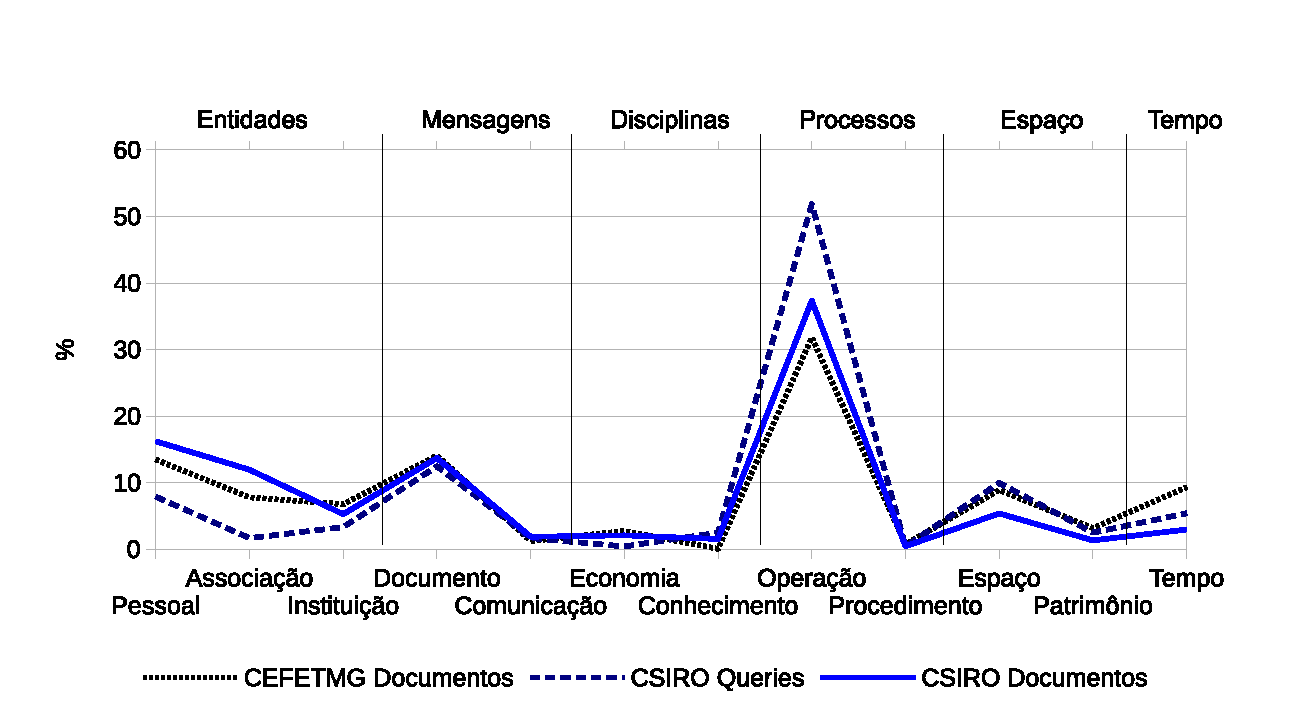
\includegraphics[width=1.0\textwidth]{fig/subjects-pt-docsqueries.eps}

	\legend{Fonte: elaborada pelo autor}
\end{figure}







\begin{figure}
	\caption{\label{fig:disp-docdoc}Dispersão da categorização de assuntos presentes em documentos do CEFETMG e da CSIRO}

	\centering
		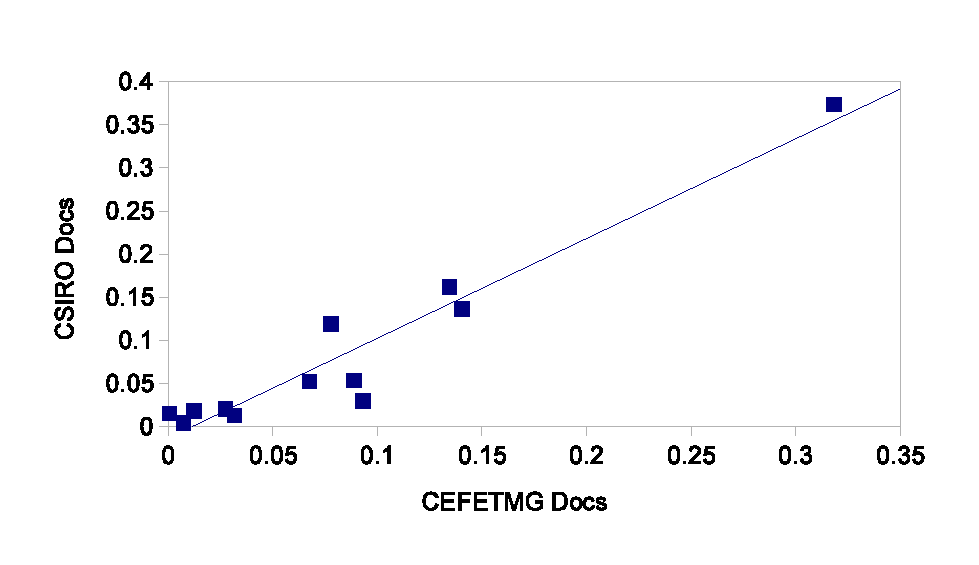
\includegraphics[width=1.0\textwidth]{fig/disp-docdoc.eps}

	\legend{Fonte: elaborada pelo autor}
\end{figure}







\begin{figure}
	\caption{\label{fig:disp-docqueryCSIRO}Dispersão da categorização de assuntos presentes em documentos da CSIRO e em queries da CSIRO}

	\centering
		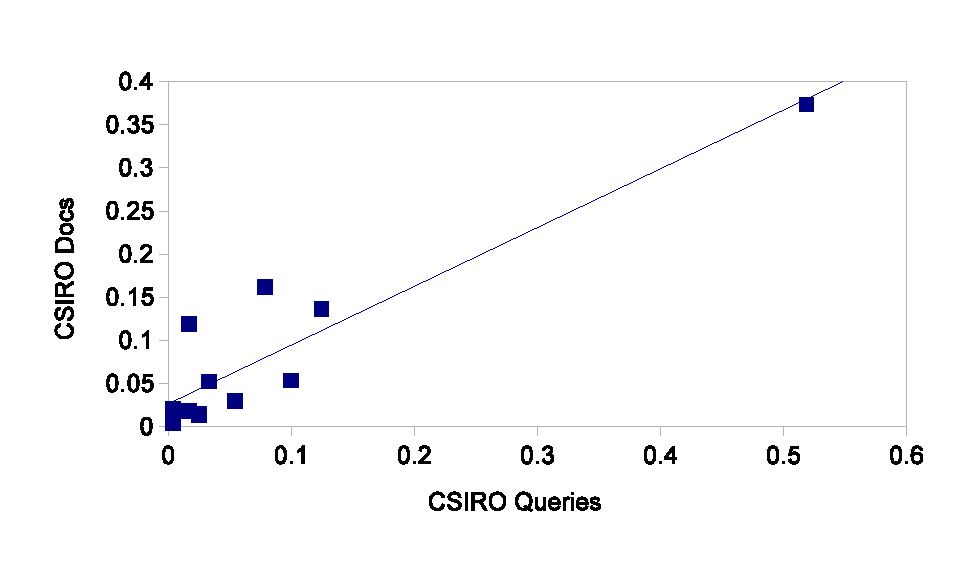
\includegraphics[width=1.0\textwidth]{fig/disp-docqueryCSIRO.eps}

	\legend{Fonte: elaborada pelo autor}
\end{figure}







\begin{figure}
	\caption{\label{fig:disp-docquery}Dispersão da categorização de assuntos presentes em documentos do CEFETMG e em queries da CSIRO}

	\centering
		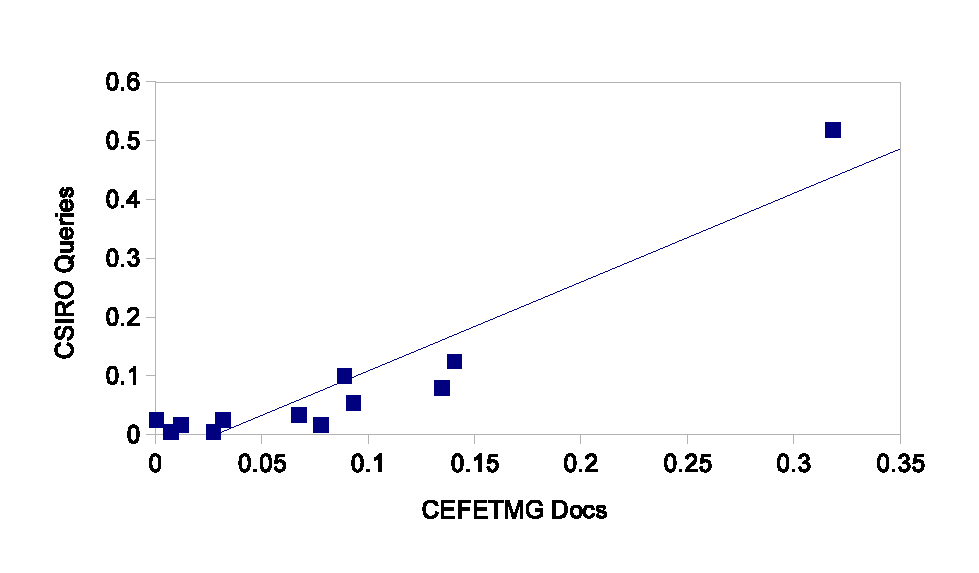
\includegraphics[width=1.0\textwidth]{fig/disp-docquery.eps}

	\legend{Fonte: elaborada pelo autor}
\end{figure}


%\textbf{Link para a próxima seção.}
Apesar de as coleções apresentarem semelhanças no nível mais alto da estrutura classificatória, as diferenças surgem e aumentam na medida em que níveis mais precisos de classificação são mobilizados. A próxima seção \ref{avaliacao-facetas} avança um nível na hierarquia da classificação e trata das facetas pelas quais cada categoria foi dividida.



\subsection{Facetas de categorias}
\label{avaliacao-facetas}

%\textbf{148 facetas resultantes.}
Ao avançar para o segundo nível da estrutura de classificação, as 12 categorias fundamentais são divididas em 148 facetas diferentes. Entre os assuntos da coleção particular, do conjunto de narrativas e \textit{queries}, e da amostra documentos da coleção pública, 97,56\%, 95,02\% e 98,13\% dos assuntos são classificados pelo menos até o nível de facetas.

%\textbf{Facetas da categoria 1.}
Em ordem alfabética, Associação é a primeira categoria, dividida em 14 facetas. Dentre elas, a faceta Parceria é a mais frequente e reúne assuntos relacionados a entidades que tenham relação de cooperação com a empresa original. Outras facetas populares em ordem alfabética são Comunicação, Concorrência, Fornecedor e Parte, relacionadas principalmente a veículos externos de difusão de informação, entidades concorrentes, entidades fornecedoras de produtos e serviços, e entidades onde a empresa possui participação societária, respectivamente. No entanto, as coleções não apresentam correlação na distribuição de facetas dentro da categoria Associação, o que sugere que as coleções tratam de interesses institucionais diferentes. Se setores compatíveis de duas ou mais organizações possuem correlação é uma questão em aberto.

%\textbf{Facetas da categoria 2.}
A segunda categoria, Comunicação, é dividida em seis facetas que representam meios de comunicação como Correspondência, Email, Internet, Rádio, Telefone e Televisão. Embora assuntos associados a esses meios de comunicação sejam comuns, especialmente endereços de email e números de telefone, não há correlação entre as coleções.

%\textbf{Facetas da categoria 3.}
A terceira categoria, Conhecimento, ganhou uma única faceta pela aplicação da técnica de desnudação. Assim, Conhecimento agrupou apenas o assunto de mais alto-nível ciência e todas as áreas do conhecimento e profissionais foram agrupadas na faceta Área. Essa estrutura é acidental e não se justifica. Uma alternativa viável é tomar a categoria Conhecimento como áreas profissionais e do conhecimento e não dividí-la em facetas, mantendo um único nível. O número de assuntos na classe Conhecimento-Área é menor que 0,07\% em todas as coleções, o que torna opcional qualquer alteração em sua estrutura.

%\textbf{Facetas da categoria 4.}
A quarta categoria, Documento, conta com 45 facetas. Não há correlação entre as coleções dentro da categoria Documento, porém as facetas mais populares em cada coleção mostram-se úteis. A faceta mais comum na coleção particular é Gênero de documento, onde estão gêneros textuais e tipos de documentos que se mostraram numerosos. Na coleção pública, por sua vez, gêneros textuais e tipos de documentos não são declarados no conteúdo de documentos, embora algumas diferenças significativas entre documentos possam ser notadas. Na coleção pública, muitos assuntos são classificados dentro da faceta Portifólio por representarem um pequeno guia (\textit{hub}) que permite a navegação para mais informação supostamente de interesse ao usuário do portifólio.

%\textbf{Facetas da categoria 5.}
Economia é a quinta categoria e foi dividida em quatro facetas. A faceta Arranjo produtivo tem elevado potencial de georreferenciamento e só foi usada na coleção particular. A faceta Atividade econômica é mais comum em todas as coleções, uma vez que atividades econômicas e profissionais são acomodadas comumente nessa faceta. As facetas Moeda e Porte acomodam poucos assuntos normalmente associados ao câmbio e à classificação de tamanho de empresas mais comum para a região onde a coleção se originou. Não há correlação entre as coleções na categoria Economia.

%\textbf{Facetas da categoria 6.}
Espaço é a sexta categoria e foi dividida em sete facetas. As facetas são resultado da desnudação baseada na hierarquia geográfica, onde temos as facetas Cidade, Continente, Distrito federal, Estado, Medida, País e Região. Apenas a faceta Medida não merece participar do renque por agrupar unidades de medida espacial ao invés de nomes de lugar. As facetas mais comuns são Cidade, Estado e País, justificado pela forma como as pessoas se referem a espaços na linguagem cotidiana quando não precisam de grande precisão geográfica. Exatamente por esse motivo, a distribuição de assuntos em facetas da categoria Espaço apresenta alta correlação positiva entre as duas coleções.

%\textbf{Facetas da categoria 7.}
A sétima categoria, Instituição, também foi dividida em sete facetas. As facetas con\-fun\-dem-se com características organizacionais bem conhecidas, como Apelido de empresa, Atualização, Cultura, Nome de empresa, Tipo de instituição, Unidade e Visão. As coleções não apresentam correlação estatística, apesar do coeficiente indicar o contrário. Entre documentos, uma correlação positiva próxima de 1 entre as amostras de documento apenas sugere que ambas as empresas contam com muitas unidades organizacionais classificadas na faceta Unidade, além de possuírem missão, visão, nome empresarial e outros atributos que realmente são características populares entre empresas. Com isso, foram as grandes estruturas organizacionais, refletidas na faceta Unidade, que determinaram a similaridade entre as duas coleções.

%\textbf{Facetas da categoria 8.}
A estrutura organizacional também interferiu em Operação. A oitava categoria foi dividida em 18 facetas, sendo que algumas facetas são atividades de unidades da instituição (Instituição-Unidade), enquanto outras são atividades de setores administrativos não presentes no organograma ou podem ser atividades administrativas presentes em diversos locais do organograma. As facetas são Atendimento, Cobrança, Compra, Controle, Desenvolvimento, Divulgação, Estoque, Financiamento, Informática, Manutenção, Orçamento, Pessoal, Produto, Segurança, Situação, Suporte à operação, Transporte e Venda. Não há correlação estatística entre as duas coleções, o que sugere que o público-alvo e/ou propósito dos documentos das coleções sejam diferentes. A hipótese de que documentos com público-alvo e propósito compatíveis apresentem alta correlação estatística merece ser verificada, algo que requer um estudo adicional fora do escopo da presente pesquisa. As facetas que em média apresentam o maior número de assuntos são Desenvolvimento, Atendimento, Pessoal e Controle, que sugerem a complexidade da comunicação no desenvolvimento de novos produtos e serviços, no atendimento de clientes, na administração de pessoas, e nos processos decisórios, respectivamente.

%\textbf{Facetas da categoria 9.}
Patrimônio é a nona categoria e foi dividida em seis facetas. As facetas são Atualização, Depreciação, Equipamento, Imóvel, Licença de software e Participação societária e não apresentam correlação estatística entre as duas coleções. De fato, bens móveis e imóveis são explicitados principalmente em função da atividade econômica, uma diferença importante entre as duas empresas investigadas. Por outro lado, a distribuição de assuntos entre essas facetas pode ajudar a classificar empresas do mesmo porte e da mesma atividade econômica. As facetas que apresentam maior número de assuntos são Imóvel e Equipamento.

%\textbf{Facetas da categoria 10.}
A décima categoria, Pessoal, foi dividida em dez facetas. As facetas são Cliente, Comunidade, Desenvolvimento, Externo, Filiação, Fornecedor, Grupo, Identificação, Profissional e Sexo. Foi registrada alta correlação positiva na distribuição de assuntos entre as facetas da categoria Pessoal, especialmente porque indivíduos têm sido representados de forma muito semelhante em documentos das coleções investigadas. As facetas com maior média de assuntos são Profissional, Externo e Cliente que acomodam indivíduos que trabalham na empresa, que colaboram com ou influenciam a empresa, e que fazem uso de serviços da empresa, respectivamente.

%\textbf{Facetas da categoria 11.}
A décima primeira categoria, Procedimento, não foi dividida em facetas ou em subfacetas. No entanto, é possível que a ausência de documentos normativos das empresas explique o fenômeno. Sua ausência sugere que as empresas não têm interesse de dar ampla publicidade a certos documentos, mantendo-os restritos exclusivamente aos funcionários para quem os documentos se destinam.

%\textbf{Facetas da categoria 12.}
Por último, as facetas da categoria Tempo são 19, sendo que as facetas Período, Ano, Calendário e Cronograma apresentaram mais assuntos. Não há correlação na distribuição dos assuntos de facetas da categoria Tempo entre as coleções.

%\textbf{Link para próxima seção.}
Apesar de as coleções apresentarem semelhanças no nível mais alto da estrutura classificatória, suas especificidades mostram-se óbvias no segundo nível de classificação. A próxima seção \ref{avaliacao-subfacetas} avança um nível na hierarquia da classificação e trata das subfacetas pelas quais cada faceta foi dividida.




\subsection{Subfacetas de facetas}
\label{avaliacao-subfacetas}

%\textbf{311 subfacetas resultantes.}
Ao avançar para o terceiro nível da estrutura de classificação, as 148 facetas discutidas na seção anterior foram divididas em 311 subfacetas. Entre os assuntos da coleção particular, do conjunto de narrativas e \textit{queries}, e da amostra documentos da coleção pública, 63,60\%, 58,09\% e 65,61\% dos assuntos são classificados pelo menos até o nível de subfacetas.

%\textbf{Não há correlação entre as subfacetas.}
Porém, comparando as duas coleções, a distribuição de assuntos em subfacetas, no terceiro nível, não apresenta qualquer similaridade. As especificidades de cada coleção tornaram-se evidentes e tentativas de acomodar assuntos de uma coleção em subfacetas comuns às duas coleções mostraram-se ineficazes.


\section{Discussões}

%\textbf{A generalização é apenas uma tentativa. Porquês de ser assim.}
%\footnote{Este parágrafo e o posterior vieram lá do início do capítulo para o fim do capítulo, como recomendou. Concordo que ficou melhor.}
A generalização do domínio corporativo apresentada é preliminar e constitui apenas uma proposta. Sua primeira restrição está na pequena razão entre o número de empresas pesquisadas, apenas duas, e o grande número de empresas existentes no mundo. Além de muito tempo necessário para analisar vários documentos e várias empresas, reunir informação de um grande número de empresas é especialmente desafiador uma vez que as empresas normalmente não revelam sua informação. Afinal, revelar informação exporia clientes, funcionários, parceiros comerciais e planos futuros \cite{bailey07csiro}. A segunda restrição está na própria natureza do domínio corporativo que reúne empresas de setores, atividades, idiomas, culturas, tamanhos e missões tão diversos. Assim, mesmo uma amostra composta de um número elevado de empresas dificilmente bastaria para representar todo o domínio corporativo e para suportar o projeto de sistemas de recuperação de informação melhores para todas as demais empresas \cite{halevy2005enterprise}. Finalmente, uma terceira restrição está na profundidade limitada da análise do domínio empreendida. Uma vez que o empirismo e métodos estatísticos não remetem ao porquê e ao limite temporal da existência de certos padrões, sua interpretação requer análise mais aprofundada, histórica e racional da natureza, do propósito e do uso da informação do domínio corporativo \cite{hjorland2002domain}, algo que mobilizaria muito mais recursos que o faz um único trabalho exploratório, por um único pesquisador.

%\textbf{Utilidade do produto da análise de domínio via análise facetada.}
Mesmo com limitações, a análise preliminar do domínio baseada na análise facetada foi útil por permitir um desenvolvimento gradual, incremental e flexível de uma classificação facetada para o domínio corporativo. Seu resultado foi uma estrutura classificatória suficiente para subsidiar a construção de um sistema de recuperação de informação corporativo que seja comum às duas empresas analisadas, mas também constitui um esquema de classificação mais facilmente ajustável às características da informação presentes em outras empresas.

%\textbf{Discussão sobre o tempo de processamento.}
O tempo de processamento da primeira fase, de documentos da coleção particular, mostrou-se muito inferior ao tempo de processamento da segunda e da terceira fases, ambas da coleção pública, mesmo para um número muito maior de ítens processados. A principal justificativa para a diferença de tempo é o conhecimento prévio do único classificador empregado sobre a empresa da coleção particular. A coleção pública requereu um tempo adicional para estudar a empresa, seus processos, a terminologia adotada, o território australiano e documentos complementares sobre o setor de atuação da empresa.

%\textbf{Discussão sobre o volume de documentos processados.}
O número de documentos processados também difere entre as duas coleções. A coleção particular apresenta um menor número de documentos se comparada à coleção pública, embora a coleção particular pareça apresentar uma maior diversidade de tipos de documentos e representar um maior número de unidades organizacionais. Por outro lado, a coleção particular exigiu a leitura de mais documentos que a coleção pública, uma vez que a última contou com um índice construído previamente por terceiros que se mostrou adequado para o objetivo de compará-las. 

%\textbf{Discussão sobre outras diferenças entre as coleções.}
Ambas as coleções também diferem em idioma, unidades organizacionais, atividades e público-alvo. Apesar dessas diferenças, os documentos processados são os mais frequentemente citados em ambas as coleções e há uma grande compatibilidade entre as facetas mobilizadas para classificar os assuntos de cada uma.

%\textbf{Discussão sobre a compatibilidade entre narrativas e documentos da própria coleção pública.}
Antes de comparar ambas as coleções, é preciso discutir a compatibilidade entre o conjunto de narrativas e \textit{queries} e a amostra de documentos da coleção pública. Para isso, uma amostra de 50 documentos da coleção pública serviu para validar as narrativas e \textit{queries} como índices para os documentos. A figura \ref{fig:disp-docqueryCSIRO} demonstra graficamente a correlação estatística entre os dois conjuntos e a alta correlação positiva sugere que seus usuários buscam e escrevem documentos mobilizando as mesmas facetas. Assim, as narrativas e \textit{queries} constituem um índice para os documentos públicos na medida em que são constituídos por termos significativos para uma necessidade informacional e uma lista de documentos que são adequados para aquela necessidade. Porém, não foram observadas diferenças na utilidade de cada uma quando comparadas isoladamente com a coleção particular.

%\textbf{Discussão sobre a compatibilidade entre as três amostras.}
Por esse motivo, a comparação entre documentos da coleção particular e narrativas e \textit{queries} da coleção pública foi equivalente àquela entre documentos da coleção particular e documentos da coleção pública. De fato, a utilidade de ambos os conjuntos da coleção pública é a mesma e qualquer um deles pode ser usado para esse estudo sem quase qualquer diferença, como ilustrado pelas figuras \ref{fig:disp-docdoc} e \ref{fig:disp-docquery}.

%\textbf{Discussão sobre a correlação entre os dois pares de amostras.}
Enquanto a figura \ref{fig:disp-docquery} compara as narrativas e \textit{queries} da coleção pública com os documentos da coleção particular, a figura \ref{fig:disp-docdoc} compara os documentos da coleção pública com documentos da coleção particular. Usando correlação de Spearman, elas apresentam um $\rho$ muito próximo, sendo respectivamente $\rho = 0,8365, n = 12, p < 0,0006932$ e $\rho = 0,8881, n = 12, p < 0,00004583$. Embora a correlação não possa ser usada para fazer generalizações sobre todo o domínio corporativo, sua medida ajuda a explicitar similaridades e diferenças entre pares de repositórios corporativos.
Adicionalmente, ambas as coleções, pública e particular, podem ser vistas como compatíveis e a alta correlação positiva demonstra que usuários diferentes têm necessidades informacionais similares com características compatíveis. As necessidades informacionais, expressadas por mensagens dos autores para os destinatários corporativos, são representadas através de um grupo de facetas para pessoas, instituições, tipos de documentos, processos, espaço e tempo. A existência das mesmas facetas tornam ambos os repositórios coleções corporativas válidas para testar sistemas de recuperação de informação, uma vez que a coleção particular se mostra válida por garantia de usuário.

%\textbf{Discussão sobre a distribuição de assuntos entre as categorias.}
Como a categoria Operação isoladamente agrupa entre 30\% e 50\%  de todos os assuntos que ocorrem nas coleções, isso explica o efeito positivo que estruturas classificatórias baseadas em atividades de negócio causam na classificação, recuperação e \textit{ranking} de documentos corporativos. As categorias Documento e Pessoal, isoladamente, agrupam um máximo de 15\% de todos os assuntos que ocorrem em cada coleção. As demais categorias em média agrupam 10\% de todos os assuntos. Essa distribuição desigual parece ter sido a motivação para o desenvolvimento de modelos de recuperação de informação corporativa baseados exclusivamente nas categorias e facetas mais populares. Por outro lado, percebe-se um grande potencial de aumento de precisão dos modelos se forem consideradas outras facetas.

%\textbf{Discussão sobre os 6 agrupamentos de categorias.}
Isso é reforçado pela existência dos seis grupos pelas quais as 12 categorias são agrupadas, como apresentado na figura \ref{fig:facetasDocsQueries}. Os seis agrupamentos de categorias são muito semelhantes às cinco categorias fundamentais de Ranganathan, sendo o grupo Entidades sociais compatível com a categoria Personalidade; os grupos Mensagens e Disciplinas científicas compatíveis com a categoria Matéria; o grupo Processos de negócios compatível com a categoria Energia; e os grupos Espaço e Tempo compatíveis com as categorias fundamentais de mesmo nome. Associando-os dessa forma a categoria fundamental energia constitui aquela com maior significado nas coleções investigadas (com cerca de 50\% dos assuntos existentes), enquanto as outras categorias fundamentais apresentam igual significado, com cerca de 10\% dos assuntos existentes, cada uma. 

%\textbf{Discussão sobre as categorias fundamentais de Ranganathan e os 6 agrupamentos de categorias como insuficientes para conclusões.}
O postulado de Categorias Fundamentais de \citeonline{ranganathan1967} em conjunto com a pequena amostra usada nesse estudo constituem evidência anedótica para uma generalização do domínio corporativo, o que requer mais estudos tomando outras coleções corporativas. Porém, ao observar a compatibilidade entre as categorias propostas e as categorias fundamentais de Ranganathan não deseja-se estabelecer nenhuma falácia genética. De fato, nenhuma conclusão para o domínio pode ser feita a partir dessa observação sobre as coleções.

%\textbf{Discussão sobre a potencial utilidade das 12 categorias para a recuperação.}
Mesmo assim, as categorias comuns às duas coleções são úteis para melhorar o modelo de recuperação de informação corporativa, tanto para as empresas a que pertencem as coleções quanto para aquelas em que sua informação apresente as mesmas facetas com distribuição compatível. As categorias do primeiro nível, por exemplo, podem produzir um impacto no modelo de recuperação de informação corporativa das duas empresas, sem distinção. As facetas e subfacetas, de segundo e terceiro nível, também podem produzir impactos no modelo de recuperação, porém de forma diferente em cada uma das coleções. %COLAR ISSO NO PAPER DO JOURNAL OF DOCUMENTATION

%\textbf{Discussão sobre restrições do modelo resultante.}
Por outro lado, o conjunto de categorias, facetas e subfacetas produzido não deve ser visto como o único ou o melhor. Todo o processamento de documentos foi realizado por um único profissional da área, algo que favorece a consistência de categorização entre coleções e assuntos, mas a utilidade da classificação resultante ainda deve ser avaliada por usuários da coleção particular ou por meio de garantia literária no caso da coleção pública. No entanto, embora outras soluções sejam possíveis pela adoção de outros profissionais-indexadores, não importa ao propósito deste trabalho avaliar a consistência inter-indexadores e nem mesmo produzir uma indexação, classificação e recuperação com o maior desempenho possível para cada coleção.
















%Deve haver um esforço de síntese das facetas das duas coleções. No entanto, devemos destacar a presença das seguintes entidades comuns às duas coleções.

%Atores sociotécnicos: funcionários, clientes, fornecedores, sistemas, setores ou departamentos, equipamentos, produtos, serviços, grupos de clientes, grupos de fornecedores, unidades, eventos, projetos e campanhas. Algumas das entidades anteriores são coleções (\textit{blackboxes}) de atores sociais e correspondem a linguagem especializadas, missões e interfaces próprias. É o caso de setores ou departamentos, produtos, serviços, grupos, unidades, eventos, projetos, campanhas.

%Linguagens: reconhecidas e diferenciadas em cada \textit{blackbox}, servem como interface entre os atores de cada uma ou entre duas \textit{blackboxes}.
%
%Redes: a intensidade da comunicação dos atores depende da importância da informação e das trocas para que a instituição realize trabalho. Intensidade, porém, não é uma medida de frequência, mas de adesão, efetividade e valor para os atores sociais.
%
%Documentos: possuem duas instâncias em nossas análises. Alguns assumem papel tão importante que tornam-se atores técnicos, sendo citados, merecendo eventos, sendo reconhecidos em vários pontos da rede. Outros possuem apenas função de suporte às trocas de mensagens entre atores sociotécnicos, servindo como canais de comunicação entre emissores e receptores.
%
%Gêneros de documentos: mostram se comuns os emails, manuais, projetos, relatórios, cartilhas, relatórios gerenciais e técnicos, cartas, memorandos, pautas de reuniões, atas, templates, páginas Web e sites, hotsites, postagens sociais, vídeos, demonstrações, artigos, planejamento de atividades, pedidos de compras, contratos de trabalho, contratos de serviços, ordens de serviço, requerimentos, protocolo, agendas, releases, clippings, ofícios, circulares, encaminhamentos, wikis, blogs, fóruns, listas, organograma, plantas civis, dentre outros.
%
%Profissões: são irrelevantes e não remetem ao domínio da área de conhecimento, mas a função profissional/social do grupo. %É o que se observa também no artigo GIC onde bibliotecários se ajustam ao grupo em que trabalham e assumem a linguagem de trabalho do grupo.
%
%Entidades: humanas (pessoas), sociais (grupos, departamentos), técnicas (equipamentos), processuais (projetos, campanhas, serviços), documentais (objetos informacionais), espaciais (espaços de trabalho), temporais (intervalos de tempo, prazos). Essas são as mais comuns.
%
%Comunicação: é muito importante estudar e compreender a comunicação informal. No entanto, nosso estudo está restrito apenas aos processos formais que registram a informação em sistemas de informação automatizados ou semiautomizados. A comunicação formal é parte da função de cada ator da instituição e representa muitas vezes  a colaboração entre os atores para realizar trabalho em um mesmo período de tempo, ou para responder a sistemas de controle formais da administração. Na primeira opção, na medida em que os atores estão próximos e o período de tempo é estreito, as comunicações tendem a ser mais informais que formais. Será por dificuldades de recuperação? Períodos maiores e redes sociais geograficamente mais espalhadas requerem uma formalização maior e um establecimento de comunicação de maior qualidade, contextualizada e facilmente recuperável a partir do sistema de recuperação de informação.
%
%Áreas de conhecimento empregadas: são as mais diversas e dependem do setor de atuação da empresa. As mais comuns são: ciências contábeis, ciências administrativas, direito, engenharias, computação, ciência da informação e biblioteconomia, medicina, psicologia.
%
%Espaços: geográficos são citados quando é área de atuação da instituição, por terem ali unidades, clientes ou fornecedores, ou concorrentes, ou parceiros. Há também os espaços físicos de trabalho, interior às unidades, com nomes que muitas vezes coincidem com os nomes de setores, departamentos, laboratórios de pesquisa, projetos, centrais de atendimento, serviços ou produtos. Documentos que tratam de trajetos ou logística costumam citar espaços geográficos intermediários que sinalizam proporções de cumprimento da trajetória, como 25\%, 50\%, 75\%, parte mais lenta, ou mais perigosa, uma rodovia, etc.
%
%Tempos: instituições contam com uma memória relativamente curta, a qual dura o tempo do processo de trabalho mais comum na instituição. Informação contábil normalmente consiste em um ano (trimestres de dois anos consecutivos) ou dois anos (ano atual e fechamento do ano anterior). Faturamento considera um período de faturamento, muitas vezes um mês para serviços e um tempo muito variável para serviços personalizados ou produção, ou entrega de produtos. Diferentes atores da instituição atuam em diferentes tempos. Após o encerramento do período e a abertura de um novo, o esperado é que o passado recente não tenha que ser recuperado. Períodos muito antigos costumam ser irrecuperáveis em sistemas automatizados, requerendo intervenção de atores para recuperá-los de arquivos.


















%\textbf{Link para o próximo capítulo.}
O capítulo \ref{prototipo} apresenta a validação de um modelo de recuperação de informação baseado na classificação facetada desenvolvida no presente capítulo. Para a validação foi implementado um protótipo funcional de sistema de recuperação de informação corporativa sobre a coleção pública. Também, foram avaliadas as expressões de busca propostas por usuários reais da coleção particular. Ambos, o protótipo e o conjunto de expressões de busca são detalhados e servem como resultados empíricos para validação da utilidade e da eficiência do modelo facetado de representação.

%um protótipo funcional de um sistema de recuperação de informação desenvolvido sobre um modelo de recuperação de informação baseado na classificação facetada desenvolvida neste capítulo. O protótipo é detalhado e avaliado através de duas implementações, uma para cada coleção, as quais servirão como base de resultados empíricos e validação da utilidade e da eficiência do modelo de recuperação.

%Novas referências:

%``[...] the even available information may be neglected (rightfully) as one may draw on one's experience (cognitive structures) and learned interpretation of one's situation. The way an assigned work task is perceived and thus formed into a personal work task depends on the actor's knowledge, which also affects the need for any additional information'' \cite[p. 133]{vakkari2005explanation}

%``Users are excluded in Lab IR, but in information seeking human characteristics are typically independent variables'' \cite[p. 133]{vakkari2005explanation}

%``There has been much debate about the nature of relevance in information retrieval, and consequently about the dependent variables in information retrieval. In lab experiments recall and precision are exclusively based on topical relevance and not the utility of documents. It is difficult to say whether retrieval by document utility rather than topicality could in any way be supported in document indexing. It is an open question'' \cite[p. 133]{vakkari2005explanation}

%\cite{vickery1955developments}

%\cite{hughes2011inter} %inter-indexer coefficient


%
%\chapter{Recuperação automatizada da informação corporativa e facetada}
%\label{prototipo}
%%%\chapter{Recuperação automatizada da informação corporativa e facetada} - manter comentado
%
%	\begin{flushright}
%		\textit{``Há apenas um bem, o saber; \\e apenas um mal, a ignorância''.\\
%		Sócrates}
%	\end{flushright}
%
%
%%\textbf{Introdução do capítulo.}
%Este capítulo apresenta dois experimentos de recuperação de informação corporativa que se utilizam das coleções particular e pública de documentos corporativos analisadas. 
%
%%\textbf{Introdução ao primeiro experimento.}
%No primeiro experimento foi observado como os usuários de informação da coleção particular constroem as expressões de busca e quais características são compartilhadas entre as expressões de busca e os documentos da coleção particular. Essa é a mesma estratégia adotada para análise e representação do domínio corporativo, descrita no capítulo \ref{analiseDominio}, mas desta vez realizada com um conjunto de usuários de informação em seu contexto de trabalho.
%
%%\textbf{Razão do primeiro experimento e diferença do experimento padrão da literatura.}
%Esta pesquisa não dispensou uma avaliação complementar àquela predominante na literatura, com a coleção particular e usuários reais, para garantir que os resultados realmente retratem as influências das características específicas da informação corporativa nos métodos de recuperação de informação em situações mais próximas da realidade corporativa. Sua principal diferença é a importância dada à análise de domínio como componente formal da construção da coleção particular, o estabelecimento dos contextos de uso mais úteis para os usuários de informação e o reconhecimento das características mobilizadas e adotadas por usuários e produtores de informação \cite{lykke2011domain}.
%
%%\textbf{Limitação do primeiro experimento.}
%Porém, embora pretenda validar as conclusões desta tese, o primeiro experimento esbarra na dificuldade de reunir usuários de informação com as mesmas características daqueles que observamos em outras empresas, e na dificuldade de ter acesso direto aos usuários de informação. Portanto, a repetibilidade dos experimentos é comprometida e o problema deve ser amenizado com a execução de experimentos adicionais.
%
%%\textbf{Introdução ao segundo experimento.}
%No segundo experimento foi implementado um protótipo de sistema de recuperação de informação corporativa (SRIC) com componentes adaptados para indexar e recuperar informação facetada. Esse segundo experimento objetivou explicitar como a organização facetada da informação influencia os diferentes componentes do SRIC. O segundo experimento fez uso dos documentos da coleção de referência da trilha \textit{Enterprise} da \textit{Text Retrieval Conference}. Também fez uso do modelo de avaliação da eficiência de indexação e recuperação \cite{balog08}, reconhecido na literatura como avaliação de \textit{Cranfield}.
%
%%\textbf{Motivo para o segundo experimento.}
%A presença de uma coleção de referência favorece a comparação de trabalhos e a definição de bases de comparação. O contrário, quando experimentos são realizados em coleções particulares, a publicação de resultados se baseia muitas vezes em informação protegida, não disponível publicamente e muitas vezes sensível. Há muitas metodologias de avaliação de sistemas de recuperação de informação \cite{irEvaluation02,evaluationWithIncompleteInformation04,bucher05,sakai08ret,DBLP:conf/clef/2008}, algumas delas bem aceitas na indústria e na academia. Porém, há limitações para avaliação de sistemas corporativos pelas mesmas metodologias, dadas suas especificidades \cite{craswell05}.
%
%%\textbf{Limitação do segundo experimento.}
%Na avaliação de \textit{Cranfield} para informação corporativa, os critérios de relevância, coleções de referência e métricas de desempenho não parecem adequados para avaliar como diferentes atores sociais recuperam informação corporativa nos mais diversos contextos de uso. Entretanto, este trabalho adotou os procedimentos e resultados de \citeonline{bailey07} e \citeonline{balog08} como base de comparação, mas reconhece a impossibilidade de concluir que aperfeiçoamentos arbitrários em um sistema de recuperação de informação, mesmo bem-sucedidos sobre a coleção pública, sejam eficientes para toda e qualquer empresa. Mesmo com essa limitação, esta tese procura interpretar a razão do sucesso e do insucesso de algumas estratégias de recuperação, usadas aqui e na literatura que baseia-se na trilha \textit{Enterprise}.
%
%%\textbf{Link para as próximas seções.}
%Os resultados sobre a coleção particular são apresentados na seção \ref{prototipo-colecaoParticular} e os resultados sobre a coleção pública são apresentados na seção \ref{prototipo-colecaoPublica}. As discussões dos resultados ocorrem isoladamente dentro das seções citadas em função das especificidades de cada experimento.
%
%
%
%
%
%
%
%
%
%\section{Experimento sobre a coleção particular}
%\label{prototipo-colecaoParticular}
%
%%\subsection{Procedimentos metodológicos}
%
%%\textbf{Caracterização do primeiro experimento.}
%No primeiro experimento, os procedimentos metodológicos empreendidos cumpriram a função de caracterizar os documentos de uma coleção corporativa e as consultas de usuários ao buscar por um conjunto de documentos. A coleção de documentos adotada é um conjunto de documentos escritos em língua portuguesa, pertencente a um campus do Centro Federal de Educação Tecnológico de Minas Gerais (CEFETMG), em Timóteo, Minas Gerais. São 1305 documentos que incluem principalmente e-mails, páginas Web, relatórios técnicos, notícias internas e externas, e pautas e atas de reunião. Os documentos foram criados entre os anos de 2007 e 2013 e têm sido acessados por seus usuários durante o período de 2012 a 2013. Esses são os mesmos documentos usados na análise preliminar de domínio apresentada no capítulo anterior.
%
%%\textbf{Caracterização da participação.}
%De uma população de sete coordenadores, cinco se prontificaram a participar da pesquisa. Eles são familiarizados com o uso dos documentos da coleção e foram solicitados a propor expressões de busca, denominadas também como simplesmente consultas neste capítulo, que levassem para os mesmos dez documentos da coleção de documentos, pré-selecionados aleatoriamente.
%
%%\textbf{Caracterização dos participantes.}
%Os cinco participantes foram coordenadores durante o período de 2007 a 2014 ou são coordenadores atualmente. Todos são professores do sexo masculino, sendo que dois deles pertencem à área de Engenharia Elétrica e três à área de Ciência da Computação. Dois concluíram o doutorado e três concluíram o mestrado antes de exercerem o cargo.
%
%%\textbf{Ambiente da participação.}
%A proposta de participação na pesquisa foi enviada através do e-mail profissional. A mensagem do e-mail trazia a proposta da pesquisa, seu formato e aspectos éticos, as instruções, exemplos de consulta e o endereço do formulário on-line através do qual as consultas deveriam ser registradas. A mensagem original encontra-se disponível no anexo \ref{anexoMensagem}. A mensagem incluiu onze documentos, um usado para algumas consultas de exemplo que simplesmente ilustravam o que constituía uma expressão de consulta, e dez que compõem a amostra. Os participantes registraram as consultas sem usar \textit{softwares} ou repositórios da empresa, tendo acesso irrestrito à Internet. Responderam a pesquisa quando estavam em casa, sem prazo limite de participação, através de um formulário eletrônico como ilustrado no anexo \ref{anexoQuestionario}.
%
%%\textbf{Definição da amostra de documentos a recuperar.}
%A escolha de documentos foi aleatória por não haver qualquer indício de vício na coleção, supostamente composta apenas por documentos conhecidos e úteis para a unidade organizacional. O número de documentos, por outro lado, foi decidido considerando a utilidade para a pesquisa e a viabilidade para os participantes. Era esperado que um número reduzido de documentos permitisse aos participantes realizar as consultas de uma única vez, sem que a participação fosse interrompida por obrigações profissionais ou domésticas.
%
%%\textbf{Condições para consulta.}
%A consulta proposta deveria ser escrita em linguagem natural, uma vez que não há vocabulário controlado para aqueles documentos. No entanto, como cada documento de interesse era consultado antes da elaboração de sua consulta, era esperado que o vocabulário presente no documento fosse adotado por todos os participantes.
%
%%\textbf{Requisitos do experimento.}
%Para reduzir algumas das limitações do método e permitir pesquisas que possam ser comparadas com a atual, os seguintes requisitos foram definidos: a amostra de documentos é aleatória; uma cópia dos documentos foi entregue aos participantes, dispensando-os de acessar qualquer repositório da empresa; os participantes foram instruídos a não usarem qualquer recurso além dos documentos providos; não foi fornecida orientação sobre como se fazer uma busca eficiente ou quais e quantos termos deveriam ser usados na consulta; e os participantes foram orientados a consumirem o tempo de dez minutos para elaborar todas as consultas.
%
%%\textbf{Descarte de um dos formulários.}
%Um dos participantes é autor desta tese e foi o responsável pela categorização dos documentos da coleção. Portanto, como o objetivo deste trabalho é comparar características dos documentos e das consultas dos usuários, seu formulário foi descartado e os resultados da pesquisa não usam as consultas propostas pelo autor. Sua participação serviu apenas para testar o formulário e estimar o tempo de resposta.
%
%%\textbf{Análise de assunto e análise facetada sobre as expressões de busca.}
%Foi feita a análise de assunto e posteriormente aplicada a análise facetada para a determinação das facetas  nas consultas de quatro participantes, totalizando 40 consultas. Como visto no capítulo anterior, os documentos foram indexados e categorizados por um único pesquisador. A indexação produziu uma lista de termos em linguagem natural que pertencem à coleção, tendo sido categorizados ao final da indexação. São as categorias e dois níveis de subcategorias os objetos de estudo neste trabalho, sendo que nem sempre os três níveis foram mobilizados. Um exemplo de termo em que apenas um nível foi mobilizado é ‘denúncia’, categorizado como Comunicação. O termo ‘departamento’ mobiliza dois níveis, a categoria Instituição e a subcategoria Unidade. O termo ‘diretor’, por sua vez, mobiliza os três níveis, a categoria Pessoal, a subcategoria Profissional e o terceiro nível Papel.
%
%%\textbf{Explicação sobre a comparação empreendida entre as expressões de busca e os documentos.}
%As categorias e subcategorias resultantes foram usadas para comparar as características dos assuntos que compõem o conteúdo dos documentos e o conteúdo das consultas dos usuários corporativos, respondendo aos objetivos deste capítulo. Para avaliar o padrão da distribuição de assuntos entre coleção e consultas foi adotado o coeficiente de correlação de Spearman. Ele se mostrou adequado para a comparação, além de não requerer uma análise estatística excessivamente complexa. Portanto, o coeficiente de Spearman também é útil para que os resultados presentes e de trabalhos futuros sejam comparados sem que os dados de empresas sejam expostos.
%
%\subsection{Resultados do experimento sobre a coleção particular}
%\label{prototipo-resultados-particular}
%
%%\textbf{Introdução aos resultados.}
%O principal objetivo deste primeiro experimento foi identificar as categorias ou características comuns a documentos corporativos e consultas de usuários enquanto buscam por documentos pertinentes em seu contexto de trabalho. Para isso, dez expressões de busca foram produzidas por quatro participantes da empresa investigada, totalizando 40 consultas. O tempo médio de produção de cada consulta foi igual a 1 minuto. A categorização dos termos presentes nas consultas foi realizada pelo mesmo indexador dos documentos, o que consumiu um tempo adicional de 2 horas e 22 minutos.
%
%\begin{figure}
%	\caption{\label{fig:avaliacaoPart-distribuicaoAssuntos}Distribuição de assuntos entre as categorias}
%
%	\centering
%		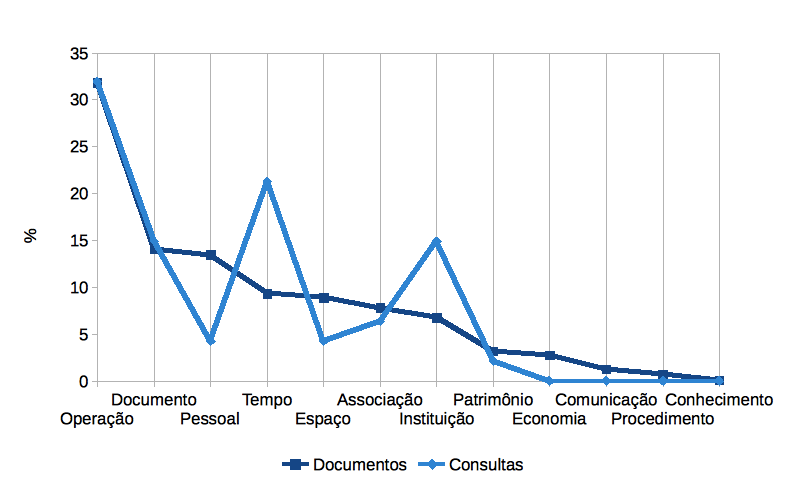
\includegraphics[width=1.0\textwidth]{fig/avaliacaoPart-distribuicaoAssuntos.png}
%
%	\legend{Fonte: elaborada pelo autor}
%\end{figure}
%
%%\textbf{Assuntos encontrados na expressão de busca e compatibilidade da distribuição entre assuntos.}
%O indexador identificou 1643 termos/assuntos diferentes em toda a coleção de documentos e 47 termos/assuntos diferentes nas consultas de usuários. Os assuntos identificados durante a indexação dos documentos e na formulação de consultas foram agrupados nas 12 categorias descobertas no capítulo \ref{analiseDominio}. A figura \ref{fig:avaliacaoPart-distribuicaoAssuntos} apresenta as categorias e a proporção de assuntos associados a cada uma delas. As categorias são Pessoal, Associação, Instituição, Documento, Comunicação, Economia, Conhecimento, Operação, Procedimento, Espaço, Patrimônio e Tempo. A proporção de assuntos em cada categoria é compatível entre a coleção de documentos e nas consultas formuladas por usuários da informação corporativa. As categorias que apresentaram maior compatibilidade entre os conjuntos avaliados são Operação, Documento, Associação e Patrimônio, com a frequência de assuntos quase idêntica entre documentos e consultas. As categorias Economia, Comunicação, Procedimento e Conhecimento, embora apresentem graficamente pontos próximos na figura \ref{fig:avaliacaoPart-distribuicaoAssuntos}, não apresentaram qualquer assunto nas consultas formuladas e portanto devem ser descartados da análise.
%
%%\textbf{Demonstração da correlação via gráfico e via coeficiente.}
%A figura \ref{fig:avaliacaoPart-correlacaoDistribuicaoAssuntos} ilustra a dispersão das frequências de assuntos em cada categoria entre os documentos e as consultas de seus usuários. A distribuição apresenta alta correlação positiva indicada por coeficiente de Spearman: $\rho(10) = 0,860912, n = 12, p = 0,0003231$, usando as 12 categorias de mais alto nível.
%
%%\textbf{Inexistência de correlação nos níveis mais baixos.}
%Por outro lado, nos níveis mais baixos da categorização, houve uma reduzida correlação positiva entre a distribuição de assuntos em facetas e subfacetas entre os documentos e as consultas. Isso sugere a inexistência de correlação estatística na medida em que o nível de classificação torna-se mais preciso.
%
%\begin{figure}
%	\caption{\label{fig:avaliacaoPart-correlacaoDistribuicaoAssuntos}Correlação da distribuição de assuntos entre categorias}
%
%	\centering
%		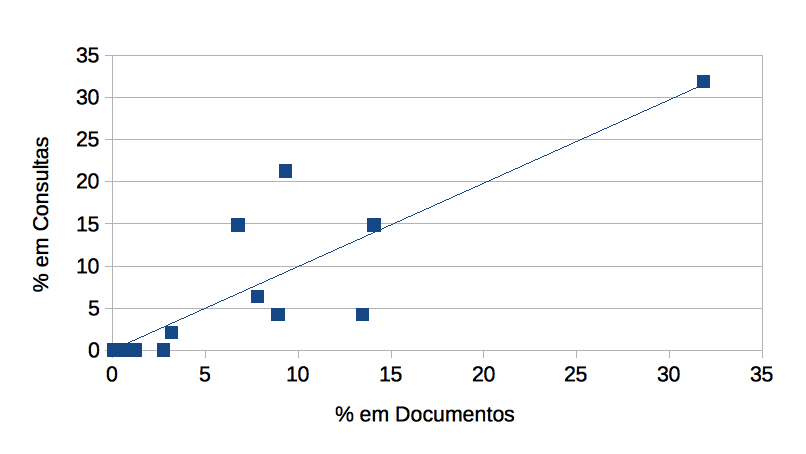
\includegraphics[width=1.0\textwidth]{fig/avaliacaoPart-correlacaoDistribuicaoAssuntos.png}
%
%	\legend{Fonte: elaborada pelo autor}
%\end{figure}
%
%%\textbf{Apresentação da tabela e explicações.}
%Analisando exclusivamente as expressões de busca, os usuários participantes fizeram uso de um total de 47 termos diferentes para elaborar as consultas que levariam aos dez documentos de interesse. A tabela \ref{termosUsuariosColecaoParticular} apresenta os termos adotados pelos usuários para os dez documentos da amostra. Para cada documento, os termos usados pelos usuários que pertencem a mesma categoria foram alinhados horizontalmente. Assim, para buscar pelo documento 1, os quatro usuários fizeram uso dos termos “congregação” e “ata” das categorias Operação e Documento. Apenas dois fizeram uso do termo “2009” e um fez uso do termo “dezembro de 2009”, ambos da categoria Tempo. Três deles fizeram uso do termo “timóteo” da categoria Espaço e “cefet” de Instituição. Dois deles fizeram uso do termo “reunião” da categoria Operação. Finalmente, apenas um deles fez uso do termo “campus” da categoria Instituição.
%
%
%
%
%%\scriptsize
%\begin{center}
%%\begin{longtable}{p{4cm}|l|l|l|l}
%\begin{longtable}{c|p{3cm}|p{3cm}|p{3cm}|p{3cm}}
%\caption[Termos usados em expressões de busca de usuários da coleção particular]{Termos usados em dez expressões de busca de quatro usuários da coleção particular}
%\label{termosUsuariosColecaoParticular}
%
%\hline \textbf{Doc.} & \textbf{Usuário 1} & \textbf{Usuário 2} & \textbf{Usuário 3} & \textbf{Usuário 4}  \\ \hline 
%\endfirsthead
%
%\multicolumn{5}{c}%
%{{\bfseries \tablename\ \thetable{} -- continuação da página anterior}} \\
%\hline \textbf{Doc.} & \textbf{Usuário 1} & \textbf{Usuário 2} & \textbf{Usuário 3} & \textbf{Usuário 4} \\ \hline 
%\endhead
%
%\hline \multicolumn{5}{r}{{Continua na próxima página}} \\ \hline
%\endfoot
%
%%\hline % Retirada para incluir Fonte.
%\endlastfoot
%
%1 & congregação \newline\newline
%ata \newline
%2009 \newline\newline
%timóteo \newline
%cefet \newline
%campus \newline
%reunião
% & 
%congregação \newline\newline
%ata \newline
%dezembro de 2009
% & 
%congregação \newline\newline
%ata \newline
% \newline\newline
%timóteo \newline
%cefet
% &
%congregação unidade \newline
%ata \newline
%2009 \newline\newline
%timóteo \newline
%cefet \newline
% \newline
%reunião
%  \\ \hline
%
%2 & regime disciplinar discente & regime disciplinar discente & 
%regime disciplinar \newline\newline
%cefet \newline
%timóteo
% & 
%regime disciplinar discente \newline
%cefetmg
% \\ \hline
%
%3 & 
%palestra \newline
%edificações \newline\newline
%timóteo \newline
% \newline
%2010
% & 
%palestra\newline
%edificações\newline\newline
%\newline
%\newline
%\newline
%incêndio
%  & 
%palestra\newline
%\newline\newline
%timóteo\newline
%cefet\newline
%\newline
%combate incêndio
%  & 
%palestra\newline
%curso técnico edificações\newline
%timóteo\newline
%cefet\newline
%\newline
%fundamentos para elaboração projeto prevenção
% \\ \hline
%
%4 &
%greve\newline
%\newline
%professor\newline
%\newline
%publicação externa\newline
%2012
% &
%greve\newline
%timóteo\newline
%professor
% &
%greve\newline
%timóteo\newline
%\newline
%cefet\newline
%\newline\newline
%\newline
%diário do aço
% &
%timóteo\newline
%\newline\newline
%cefet\newline
%\newline
%\newline\newline
%\newline
%dois meses de paralisação
% \\\hline
%
%5 &
%estrutura organizacional\newline
%timóteo\newline
%\newline
%2014
% &
%organograma\newline\newline
%timóteo
% &
%estrutura organizacional\newline
%timóteo\newline
%cefet
% &
%estrutura organizacional\newline
%timóteo\newline
%cefet
% \\\hline
%
%6 &
%requerimento\newline
%coordenação de programa de estágios
% &
%requerimento\newline
%\newline
%\newline\newline\newline
%\newline
%estágio\newline
%carta
% &
%requerimento\newline
%\newline\newline\newline
%cefet\newline
%timóteo\newline
%estágio
% & 
%requerimento\newline
%coordenação programa estágio\newline\newline
%cefet\newline
%timóteo
% \\\hline
%
%7 &
%\newline
%curso\newline\newline
%pró-técnico\newline
%2009\newline
%\newline
%\newline
%\newline
%publicação externa
%  &
%vestibular\newline
%\newline\newline
%pró-técnico\newline
%2010
% & 
%vestibular\newline
%\newline
%\newline\newline
%\newline
%prefeitura\newline
%timóteo\newline
%cefet
% & 
%vestibular\newline
%curso preparatório\newline
%\newline
%\newline
%prefeitura\newline
%timóteo\newline
%cefet
% \\\hline
%
%8 & 
%fórum dos coordenadores\newline
%ata\newline
%\newline
%\newline
%\newline
%recuperação\newline
%sistema
% & 
%fórum\newline\newline
%ata\newline
%março de 2013
% & 
%fórum\newline\newline
%ata\newline
%\newline
%cefet\newline
%timóteo
% & 
%fórum coordenadores\newline
%ata\newline
%2013\newline
%cefet\newline
%timóteo\newline
%\newline
%\newline
%2\newline
%reunião
% \\\hline
%
%9 & 
%palestra\newline
%mark\newline
%\newline
%\newline
%2013\newline
%realidade aumentada
% & 
%palestra\newline
%mark
% & 
%palestra\newline
%mark\newline
%cefet\newline
%timóteo
% & 
%palestra\newline
%mark\newline
%cefet\newline
%timóteo\newline
%\newline
%\newline\newline
%prof
% \\\hline
%
%10 & 
%congresso\newline
%abm\newline
%\newline
%\newline
%curso técnico em metalurgia
% & 
%congresso\newline
%abm\newline
%\newline
%expominas
% & 
%congresso\newline
%abm\newline
%cefet\newline
%timóteo
% & 
%congresso\newline
%abm\newline
%cefet\newline
%timóteo\newline
%\newline\newline
%64
% \\\hline
%
% \hline \multicolumn{5}{l}{Fonte: Elaborada pelo autor.}
%
%\end{longtable}
%\end{center}
%%\normalsize
%
%
%
%
%
%
%%\textbf{Apresentação do número de termos das 10 consultas.}
%As consultas apresentaram grandes diferenças entre si. A consulta 1 foi formulada com o maior número de termos, 5 em média, e com o maior desvio-padrão 1,825. A consulta 2, por sua vez, foi formulada com o menor número de termos, 1,75 em média. Como um todo, as consultas foram formuladas com um número médio de termos igual 3,625, com desvio-padrão de 1,314. As discussões de resultados deste experimento são apresentadas na seção \ref{prototipo-discussoes-particular}.
%
%
%
%
%
%
%
%\subsection{Discussões de resultados sobre a coleção particular}
%\label{prototipo-discussoes-particular}
%
%%\textbf{Introdução da seção.}
%A seção \ref{prototipo-resultados-particular} apresentou os resultados da categorização de assuntos dos documentos corporativos e das consultas formuladas pelos usuários da coleção particular pesquisada. Os resultados atendem ao objetivo de explicitar características comuns aos documentos e consultas por meio da distribuição de assuntos entre as categorias identificadas.
%
%%\textbf{8 categorias descobertas.}
%Foram identificadas 12 categorias a partir da análise na análise preliminar de domínio (capítulo \ref{analiseDominio}). Portanto, a análise de domínio preliminar aconteceu antes de considerar os usuários da coleção particular e suas consultas como objeto de estudo. A amostra de consultas, apesar de reduzida, foi suficiente para determinar a compatibilidade das categorias entre o conjunto de documentos e de consultas. Porém, ao incluir as consultas de usuários foram obtidos 47 termos/assuntos, categorizados por meio de apenas oito das 12 categorias originalmente encontradas nos documentos. 
%
%%\textbf{Discussão sobre as 8 categorias e sobre a compatibilidade entre documentos e expressões de busca.}
%Em metade das oito categorias a frequência de assuntos que ocorrem na coleção de documentos e nas consultas é quase idêntica. É esse resultado que justifica a adoção do método em pesquisas futuras e merece ser verificado em outras empresas e em outras situações de trabalho da mesma empresa investigada. No entanto, a frequência desigual entre as amostras de algumas categorias, os pontos mais distantes da linha de tendência da figura \ref{fig:avaliacaoPart-correlacaoDistribuicaoAssuntos}, não significa prontamente que tais categorias sejam menos importantes. A figura \ref{fig:avaliacaoPart-distribuicaoAssuntos} mostra as categorias Tempo e Instituição, por exemplo, com mais de 15\% dos assuntos informados nas consultas pelos usuários. Claramente, isso significa que o tempo e as unidades organizacionais são mais importantes no momento de consultar, restringindo a informação que se deseja obter, do que no momento de produzir, quando o tempo segue seu curso natural e as unidades organizacionais têm um ciclo de vida mais longo.
%
%%\textbf{Discussão sobre Pessoal.}
%Outra categoria onde a frequência não é compatível é a Pessoal. Em uma amostra tão reduzida, os participantes fizeram pouco uso de nomes de pessoas e papeis desempenhados na instituição. E como citado acima, fizeram uso intenso de assuntos da categoria Instituição aparentemente para impor um filtro artificial à informação, uma vez que reconhecem que seus documentos de interesse constituem uma fração muito pequena da miríade de documentos que sua instituição tem produzido ao longo dos anos. Tais fenômenos não ocorreram entre os assuntos presentes nos documentos. Muitos atores sociais apareceram nas mensagens e muitos são os seus papeis e cargos. Em número muito inferior ao de pessoas, as unidades organizacionais estiveram sempre presentes, mas se repetiram em vários documentos da empresa, minimizando sua participação no conjunto de assuntos presentes nas mensagens.
%
%%\textbf{4 categorias sem assuntos.}
%Por outro lado, quatro categorias não apresentaram assuntos em consultas, a saber: Economia, Comunicação, Procedimento e Conhecimento. Isso se justifica pelo tamanho da amostra limitado a apenas dez documentos de interesse. O acréscimo de mais documentos certamente produziria a ocorrência de assuntos de categorias não mobilizadas.
%
%%\textbf{Discussão sobre a correlação incluindo as 12 categorias, ao invés das 8 categorias.}
%De qualquer forma, a correlação, ilustrada na figura \ref{fig:avaliacaoPart-correlacaoDistribuicaoAssuntos}, a partir das 12 categorias e não apenas das oito que apresentaram assuntos nas duas amostras, confirma a compatibilidade da frequência de assuntos em categorias entre o conteúdo dos documentos e o conteúdo das consultas formuladas pelos usuários. As quatro categorias em que não houve assunto entre as consultas também apresentaram escassez de assuntos (abaixo de 5\%) entre os documentos, como também se observa na figura \ref{fig:avaliacaoPart-distribuicaoAssuntos}.
%
%%\textbf{Categorias que têm 50\% dos assuntos.}
%As categorias mais numerosas foram Operação, Documento e Pessoal, que juntas correspondem a aproximadamente 50\% de todos os assuntos tratados nos documentos e propostos por usuários nas consultas. Isso explica o porquê de os sistemas de recuperação de informação corporativa atuais serem principalmente baseados em ontologias corporativas mais generalistas, em classificação de documentos por seu tipo ou gênero, e em reconhecimento de pessoas, especialmente especialistas e autoridades da empresa. Falta responder se a outra metade de assuntos tem sido considerada por indexadores intelectuais e automáticos apenas como termos comuns em uma busca em texto completo ou como características especiais da informação corporativa.
%
%%\textbf{Discussão sobre quantidade de termos.}
%A quantidade de termos usados nas consultas foi cerca de 1,6 vezes maior que a média encontrada na literatura para usuários da Web, sendo que apenas 32,2\% das consultas apresentaram três ou mais termos \cite{relevantEnterpriseData11,spink2001searching}. No entanto, a maior incompatibilidade é a própria definição do conceito de termo, sendo usado na maioria das vezes como sinônimo de qualquer sequência de caracteres alfanuméricos, uma palavra \cite{spink2001searching}. Comparando dessa forma, o número de palavras usadas por participantes é ainda maior, em média 4,7 palavras por consulta, com desvio-padrão de 1,713, duas vezes maior que a média de 2,16 palavras por consulta na Web.
%
%%\textbf{Consideração sobre como parte da literatura apresenta a quantidade de termos e a escolha da metodologia de contagem que este trabalho usa.}
%Entretanto, considerar ``new york'' como dois termos, ao invés de um, não parece apropriado e muito menos necessário. Entre os 50 pares mais frequentemente encontrados por \citeonline{spink2001searching} também estão “united states”, ``real estate'', ``new jersey'', ``north carolina'', ``for sale'', ``university of'', ``home page'', ``high school'', ``university state'' e ``chat rooms'', todos candidatos a representarem apenas um termo composto por duas ou mais palavras, algo trivial de resolver por meio de um dicionário. Assim, comparar o número de termos deste trabalho com o número de palavras presente na literatura é mais apropriado e nosso número 1,6 vezes maior parece compatível.
%
%%\textbf{Hipótese para o número de termos na Web e na busca corporativa ser compatível.}
%Uma hipótese útil refere-se ao comportamento do usuário em motores de busca na \textit{Web} estar sendo transferido para sistemas de recuperação de informação dentro da empresa. Isso pode ser verdade especialmente quando observados usuários sem treinamento para o uso do sistema de recuperação de informação corporativa ou sem formação acadêmica que o especialize a recuperar informação específica.
%
%%\textbf{Consideração sobre a categoria espacial encontrada na literatura para expressões de busca na Web e no ambiente corporativo.}
%Por outro lado, a categorização dos termos elaborados nas consultas apresenta valores que diferem de resultados vistos na literatura para \textit{Web}. \citeonline{borges07} sugerem que entre 14 e 18\% das consultas formuladas na \textit{Web} apresentam termos da categoria Espaço. Em nosso contexto corporativo, os usuários 3 e 4 usaram um termo da categoria Espaço em todas as consultas, sempre em conjunto com um termo da categoria Instituição com o propósito de ajudar o sistema a recuperar apenas informação da unidade organizacional em que trabalham. Porém, desconsiderados os usuários 3 e 4, em 50\% das consultas pelo menos um dos demais usuários fez uso de um termo da categoria Espaço aparentemente sem esse propósito.
%
%%\textbf{Consideração sobre a categoria temporal encontrada na literatura para expressões de busca na Web e no ambiente corporativo.}
%Além da categoria Espaço, os usuários fizeram uso de muitos assuntos da categoria Tempo para formular as consultas. Em oito das dez consultas, pelo menos um usuário fez uso de um termo da categoria Tempo, o que sugere que a classificação temporal de documentos corporativos seja essencial. Os usuários fizeram uso do tempo para filtrar a informação que sabem ser abundante ou recorrente, para atingir o mais antigo ou o mais recente. Na \textit{Web}, estudos como o de \citeonline{campos2011temporal} sugerem que menos de 1,5\% das consultas façam uso de termos explícitos da categoria Tempo.
%
%%\textbf{Consideração sobre o uso do espaço nas expressões de busca e a motivação para uma classificação facetada.}
%Porém, a classificação espacial não se bastaria de um simples atributo `local'. Acostumados a buscar em texto completo, os usuários fizeram um uso de localidade que pode ser melhor explorada através de uma classificação facetada. Na busca pelo documento 10, os usuários 2, 3 e 4 usaram localidades diferentes. Nesse caso, o evento aconteceu no endereço ``expominas'', que não está localizado em ``timóteo''. Porém, os usuários 3 e 4 tentaram recuperar um documento que descreve a participação de pessoas de ``cefet timóteo'' no evento ``congresso abm'', enquanto o usuário 2 tenta recuperar um documento que descreve o evento ``congresso abm'' que aconteceu em ``expominas''.
%
%%\textbf{Consideração sobre o uso do tempo nas expressões de busca e a motivação para uma classificação facetada.}
%Também, a classificação temporal não se basta de um único atributo `data de criação' pelo mesmo motivo. Para buscar pelo documento 7, os usuários 1 e 2 fizeram uso de dois termos diferentes para a mesma categoria Tempo, ``2009'' e ``2010''. O uso de anos diferentes se explica ao observar a ordem em que foram usados na expressão de busca. O primeiro como ``pró-técnico 2009'', o segundo como ``pró-técnico vestibular 2010'', significando que o pró-técnico aconteceu em 2009 para um vestibular que ocorreria em 2010 ou cujo ingresso ocorreria em 2010. Isso remete à importância de compreender como os usuários de informação constroem a mensagem que a expressão de busca carrega, associando corretamente tempo e espaço às entidades certas por meio de uma classificação facetada.
%
%%\textbf{Conclusão e link.}
%De fato, se a informação corporativa, as buscas e seus usuários reúnem tantas particularidades que não são compartilhadas com outros contextos de busca, como da própria \textit{Web}, são necessários métodos e tecnologias especiais para tornar o processo de recuperação mais eficaz e eficiente. Na seção seguinte, \ref{prototipo-colecaoPublica}, é apresentado o experimento realizado sobre a coleção pública.
%
%
%
%
%
%
%
%
%
%
%
%\section{Experimento sobre a coleção pública}
%\label{prototipo-colecaoPublica}
%
%%\textbf{Introdução ao segundo experimento.}
%No segundo experimento, os procedimentos metodológicos empreendidos cumpriram a função de avaliar a eficiência da indexação e da recuperação de documentos da coleção corporativa de referência, denominada como coleção pública, em algumas partes desta tese, por estar disponível desde o ano de 2007 para toda a comunidade científica. 
%
%%\textbf{Re-apresentação da coleção pública apenas para favorecer o leitor.}
%A coleção pública é um conjunto de documentos escritos em língua inglesa, pertencente à \textit{Commonwealth Scientific and Industrial Research Organisation} (CSIRO). São 370715 páginas \textit{Web} de alguns dos repositórios da empresa, todos disponíveis para o público interno e externo. Esses são os mesmos documentos usados na análise preliminar de domínio apresentada no capítulo anterior. 
%
%%\textbf{Re-apresentação das narrativas apenas para favorecer o leitor.}
%A coleção de referência também inclui um conjunto de 77 narrativas e 77 \textit{queries} disponibilizadas por funcionários da CSIRO como as questões mais frequentemente feitas por clientes e respondidas pela CSIRO \cite{bailey07csiro}. As narrativas correspondem a uma questão de exemplo escrita por um cliente e enviada para funcionários da CSIRO. Para responder a questão do cliente, um funcionário deveria realizar uma busca no sistema de recuperação de informação da empresa. Essa busca é constituída por um exemplo de \textit{query}, ou expressão de busca, que retorna documentos pertinentes para responder a questão.
%
%%\textbf{Explicação sobre o método de avaliação de eficiência da recuperação.}
%O método de avaliação da eficiência consiste em realizar a indexação automática e, em seguida, realizar cada uma das 77 buscas em um sistema automatizado de recuperação de informação (SRI). A partir das 77 respostas obtidas através do SRI, se deve comparar a lista de documentos retornados com a lista de documentos previamente classificados como não relevantes, relevantes ou altamente relevantes para cada necessidade de informação.
%%A classificação de documentos da CSIRO não foi exaustiva.
%
%%\textbf{Medida de eficiência e comparação entre SRI.}
%Naturalmente, a medida da eficiência do SRI dá-se pela recuperação do maior número possível de documentos considerados altamente relevantes, especialmente nas primeiras posições do \textit{ranking}, seguidos por documentos considerados relevantes. Documentos considerados não relevantes e/ou documentos não classificados para uma dada necessidade não deveríam ser recuperados, especialmente nas primeiras posições do \textit{ranking}. Esse método de avaliação permite distinguir empiricamente qual sistema de recuperação de informação é mais eficiente para uma dada coleção e para um conjunto de necessidades de busca, não garantindo eficiência para qualquer outra coleção e para quaisquer outras necessidades de busca, da mesma coleção ou de outras.
%
%%Supondo a existência de uma coleção e de necessidades de informação especificadas sem qualquer viés, esse método de avaliação supostamente indicaria 
%
%%\textbf{Link para próximas seções.}
%O projeto do protótipo de sistema de recuperação de informação corporativa e facetada é tratado na seção \ref{prototipo-arquitetura}. O método de indexação de informação corporativa facetada é tratado na seção \ref{prototipo-indexacao}. Finalmente, o método de processamento automático de consultas é tratado na seção \ref{prototipo-consultas}.
%
%
%
%%\subsection{Procedimentos metodológicos}
%
%\subsection{Arquitetura do protótipo de sistema automatizado de recuperação de informação corporativa}
%\label{prototipo-arquitetura}
%
%%\textbf{Características do protótipo.}
%O protótipo de sistema de recuperação de informação foi implementado sobre a Apache Lucene\footnote{Apache Lucene pode ser obtida em http://lucene.apache.org}, uma biblioteca de \textit{software} implementada na linguagem de programação Java destinada para indexação e recuperação automáticas de documentos.
%
%%\textbf{Métodos implementados.}
%Para indexar e recuperar informação corporativa facetada, foram usados métodos comuns de indexação e recuperação de informação, com pequenas alterações que suportassem a informação corporativa, organizada em facetas social, espacial e temporal. Essa estratégia é a mais comum na literatura ao permitir uma prototipação mais simples que sirva como prova de conceito, sem consumir tempo e esforço de programação com os componentes básicos do sistema de recuperação de informação \cite{anastacio09}.
%
%%\begin{figure}
%%	\caption[Arquitetura de sistema de recuperação de informação]{\label{fig:ir-architecture}Arquitetura de sistema de recuperação de informação.}
%%
%%	\centering
%%		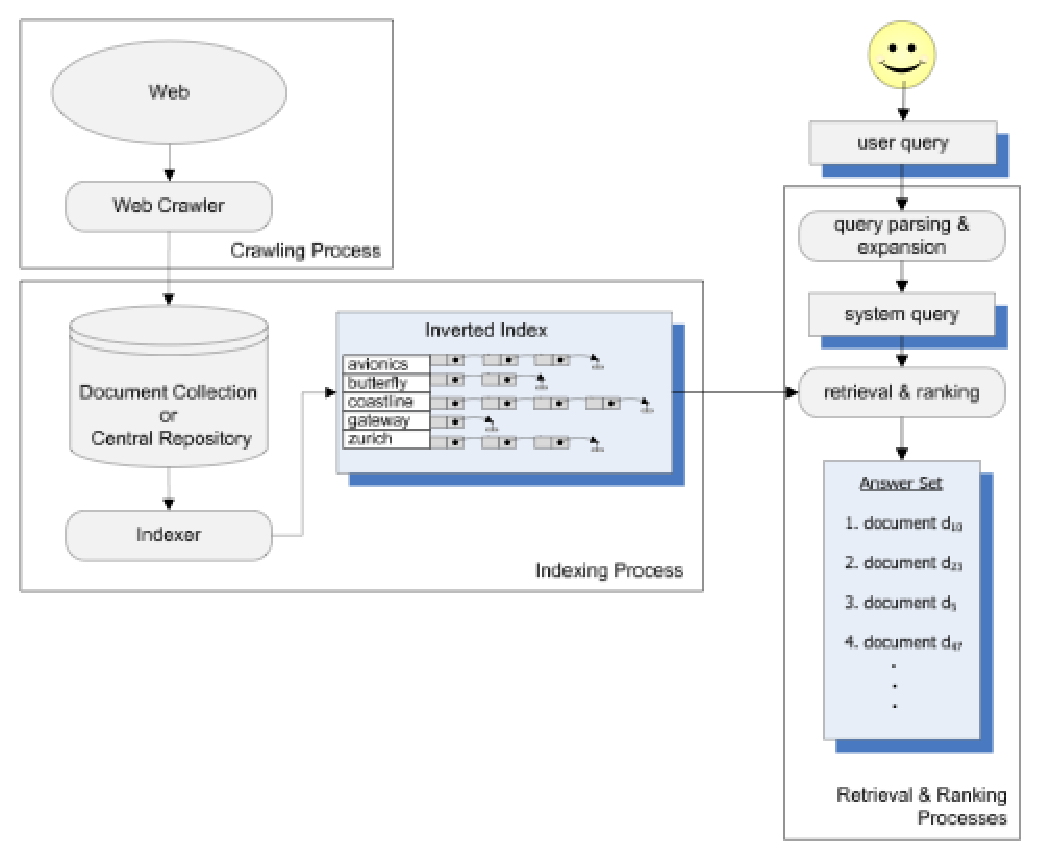
\includegraphics[width=1.0\textwidth]{fig/ir-architecture.eps}
%%
%%	\legend{Fonte: \cite{mir2ed}}
%%\end{figure}
%
%%\textbf{Explicação da figura.}
%A figura \ref{fig:ir-architecture} apresenta a arquitetura de um sistema de recuperação de informação, o qual pode ser alterado para indexar e recuperar informação corporativa usando uma estrutura facetada sem alterações em sua arquitetura.
%
%%\textbf{Ausência de coletor de documentos.}
%Este trabalho adotou a coleção pública já pronta, sem a necessidade que um coletor (\textit{Web Crawler}) fosse implementado e usado. Assim, o primeiro componente implementado foi um indexador (\textit{indexer}).
%
%%\textbf{Componente Indexador.}
%O indexador automático (\textit{indexer}) é responsável por representar a coleção de documentos através de índices. Foram implementadas as seguintes estruturas de dados para representar ítens reconhecidos no conteúdo dos documentos: um arquivo invertido (\textit{inverted index}), estrutura padrão do Apache Lucene, para representar os termos; um \textit{gazetteer} para representar os termos geográficos; uma linha do tempo para representar as datas; e listas para representar atividades econômicas, documentos, pessoas, unidades organizacionais e patrimônio (equipamentos e \textit{softwares}).
%
%%\textbf{Componente de interface de busca.}
%O usuário de informação realiza sua busca através de uma interface com o usuário. Foi implementada uma interface com o usuário exclusivamente para testes eventuais do protótipo de sistema de recuperação de informação. Para uma execução mais rápida das 77 buscas, foi implementado um componente de processamento não assistido de consultas. Esse componente não faz parte de um sistema clássico de recuperação de informação e, portanto, não está presente na figura \ref{fig:ir-architecture}.
%
%%\textbf{Componente Processador de Expressão de busca.}
%O processador de expressão de busca (\textit{query parsing \& expansion}) é responsável por reconhecer as palavras-chaves informadas pelo usuário de informação e por reescrever a expressão de busca do usuário, incluindo ou retirando termos para aumentar a eficácia da recuperação. Neste componente foi implementado um método para reconhecer a faceta à qual pertence cada termo, produzindo uma reescrita mais elaborada. Em caso de expansão, exclusão ou alteração de termo, a operação ocorre exclusivamente dentro da faceta correspondente.
%
%%\textbf{Componente de recuperação de informação.}
%A expressão de busca final deve ser processada pelo componente de recuperação e ordenação (\textit{retrieval \& ranking}). O componente é responsável por recuperar os documentos supostamente de interesse e ordená-los em função de uma métrica de relevância. A métrica de relevância adotada é a \textit{term frequency-inverse document frequency} (TF-IDF), padrão no Apache Lucene, sem associar pesos diferentes para as facetas.
%
%
%
%\subsection{Indexação automática da informação corporativa}
%\label{prototipo-indexacao}
%
%%\textbf{Tempo de indexação.}
%A indexação automática da coleção pública consumiu um tempo total de 680856 milissegundos (ou 11,3476 minutos) em um computador com \textit{chipset} de 32 bits; processador Intel Core 2 Duo, P8400, com frequência de 2268 MHz; disco rígido de 160GiB, com 5400 rotações por minuto; memória principal de 4 GiB, frequência de 800 MHz; e sistema operacional Linux 32 bits.
%
%%\textbf{Índices do SRI.}
%O indexador automático representou a coleção por meio de oito índices, algo possível após a leitura técnica empreendida no capítulo anterior. O primeiro índice, um arquivo invertido, indexou todos as palavras presentes no conteúdo dos documentos. O segundo índice, um \textit{gazetteer}, indexou países, estados, territórios australianos, cidades, oceanos e mares, equipamentos urbanos e outras feições geográficas úteis, entre naturais, artificiais e cartográficas. Todas as referências geográficas indexadas estão presentes nas tabelas \ref{assuntosCSIROquery} e \ref{assuntosCSIROdocs}. O terceiro índice, uma linha do tempo, indexou as referências a anos encontradas no conteúdo dos documentos, utilizando-se de uma estratégia ingênua de associar qualquer palavra, ou \textit{token}, formada por quatro números como uma suposta referência a um ano. Os índices restantes, formados como listas ordenadas alfabeticamente, indexaram as referências às atividades econômicas, documentos, pessoas, unidades organizacionais e patrimônios da empresa.
%
%%\textbf{Sem processamento de linguagem natural.}
%Neste protótipo, nenhum índice dependeu do processamento de texto para interpretar as referências e aumentar sua precisão. Isto é, referências tais como "ano passado", "década anterior", "próximo a Sydney", "entre Sydney e Camberra" e outras são indexadas de maneira imprecisa, sem tratamento espaço-temporal do texto. Essa omissão não constitui uma recomendação para o projeto de um sistema de recuperação de informação, mas uma simples limitação do protótipo.
%
%%\textbf{Link para a próxima seção.}
%Na próxima seção são apresentadas as expressões de busca e de que forma ocorreu o processamento das expressões de busca para realizar a recuperação de informação da coleção pública.
%
%
%
%\subsection{Processamento automático de consultas}
%\label{prototipo-consultas}
%
%%\textbf{Modelo de interação avaliado.}
%Em uma parcela dos sistema de recuperação de informação, o usuário deve traduzir sua necessidade de informação em palavras-chaves na forma de uma expressão de busca. Dado um conjunto de palavras-chaves, o sistema de recuperação de informação deve converter as palavras-chaves em uma lista ordenada de documentos de interesse. É esse modelo de interação e de recuperação de informação corporativa que foi avaliado na trilha \textit{Enterprise} da \textit{Text Retrieval Conference} até o ano de 2008.
%
%%\textbf{Explicação sobre a estratégia de busca facetada usando um local.}
%Porém, no protótipo corporativo e facetado implementado nesta tese, termos fornecidos pelo usuário são convertidos em facetas antes de se executar a recuperação. Assim, não se busca por um termo ``victoria'' em documentos. Ao invés disso, se busca pela faceta Estado dentro dos documentos, usando a cadeia Melbourne, Victoria, Vic, Australia e Oceania como possíveis valores para a faceta, ou usando outros valores de outras facetas do renque.
%Dessa forma, mesmo que Victoria não exista em qualquer documento, como a categoria Estado está presente, podem ser utilizados os estados das unidades organizacionais da empresa, os estados dos funcionários, dos projetos ou de outras entidades corporativas. Referências a Victoria são buscadas indiretamente.
%
%%\textbf{Explicação sobre a estratégia de busca usando um nome de pessoa.}
%Outro exemplo é o nome ``John''. Embora John seja um termo, o objeto de interesse pode ser a faceta cliente, faceta funcionário, ou a faceta Pessoa externa. Assim, são adotadas listas de funcionários, de clientes e de colaboradores, especialmente aquelas em que algum John exista. 
%
%%\textbf{Implicações dessa estratégia de busca em outros modelos de interação.}
%Essa estratégia também pode favorecer o \textit{browsing}  da coleção, em uma possível navegação facetada. Nesse modelo de interação com o usuário, critérios de ordenação são diferentes para cada expressão de busca, especialmente naquelas em que alguma categoria seja mais importante que as outras. Assim, Funcionários assumiriam ordem alfabética. Relatórios assumiriam ordem crescente de ano. Unidades organizacionais assumiriam ordem da mais importante para a menos importante, ou da mais próxima para a mais distante do usuário da informação. Porém, apenas a recuperação da informação facetada foi implementada no escopo dessa tese para buscar sua validação através da avaliação da trilha \textit{Enterprise}. Pois não há detalhes suficientes na trilha para avaliar diferentes critérios de ordenação e diferentes interfaces de usuário.
%
%% Expressões de busca
%
%%\textbf{Tabela original de 77 expressões de busca.}
%A tabela \ref{tabQueriesOriginais} apresenta as 77 expressões de busca fornecidas juntamente com a coleção pública. Embora as narrativas, que explicam as expressões de busca, tenham sido estudadas no capítulo anterior, elas não foram adotadas na avaliação da recuperação. As 77 expressões de busca foram submetidas para um sistema de recuperação de informação, usando método de similaridade \textit{text frequency-inverse document frequency} (TF-IDF).
%
%%\scriptsize
%\begin{center}
%%\begin{longtable}{p{4cm}|l|l|l|l}
%\begin{longtable}{c|p{6cm}}
%\caption[Expressões de busca originais da coleção pública]{Expressões de busca originais da coleção pública}
%\label{tabQueriesOriginais}
%
%\hline \textbf{Query} & \centering \textbf{Expressão de busca original} \\ \hline 
%\endfirsthead
%
%\multicolumn{2}{c}%
%{{\bfseries \tablename\ \thetable{} -- continuação da página anterior}} \\
%\hline \textbf{Query} &  \centering \textbf{Expressão de busca original} \\ \hline 
%\endhead
%
%\hline \multicolumn{2}{r}{{Continua na próxima página}} \\ \hline
%\endfoot
%
%%\hline % Retirada para incluir Fonte.
%\endlastfoot
%
%
%
%
%51 & weatherwall \\
%52 & solve magazine \\
%53 & selenium soil \\
%54 & the heat is on \\
%55 & case moth identification \\
%56 & 12345+ \\
%57 & fast instruments \\
%58 & wood borer treatment \\
%59 & vinelogic cd \\
%60 & algae hydrogen powered cars \\
%61 & wheel motor \\
%62 & climate change hops \\
%63 & vinegar bugs \\
%64 & ant identification \\
%65 & recruitment \\
%66 & chilli paste preservatives \\
%67 & sydney ocean temperatures \\
%68 & sea level changes East Coast \\
%69 & magnesium supplement \\
%70 & information technology jobs \\
%71 & termite wings \\
%72 & biodegradable materials \\
%73 & postdoctoral bioinformatics \\
%74 & rene van berkel \\
%75 & water conservation industry \\
%76 & electric vehicles \\
%77 & climate change \\
%78 & pem micro fuel cells \\
%79 & internship \\
%80 & biodiversity \\
%81 & artificial photosynthesis \\
%82 & total wellbeing diet seafood \\
%83 & contact scientist \\
%84 & drought nsw \\
%85 & water level property \\
%86 & rabies test \\
%87 & treated timber edible plants \\
%88 & improving the built environment \\
%89 & postdoctoral \\
%90 & plant heavy metal binding proteins \\
%91 & ultracapacitors \\
%92 & cane toad photo \\
%93 & annual report \\
%94 & ants \\
%95 & plant gene technology \\
%96 & ocean floor map \\
%97 & shipping container simulate \\
%98 & insect identification \\
%99 & training coordinator \\
%100 & water food production \\
%101 & trials weight loss \\
%102 & nathers accurate \\
%103 & forensic science workshop \\
%104 & uranium reserves \\
%105 & venture capital investment \\
%106 & biodegradable plastic \\
%107 & total wellbeing diet book 2 exercise \\
%108 & millipede control \\
%109 & employment aquaculture \\
%110 & postdoctoral mathematics \\
%111 & salinity wa \\
%112 & mineral energy resources Australia \\
%113 & sea levels \\
%114 & millipedes \\
%115 & hybrid cars \\
%116 & friction coal crush \\
%117 & freon climate change \\
%118 & termite bait box \\
%119 & melbourne events calendar \\
%120 & bubbles ice image \\
%121 & australia population \\
%122 & images \\
%123 & website feedback \\
%124 & euclid eucalypts \\
%125 & cervical cancer vaccination \\
%126 & fish oil \\
%127 & government funding \\
%
%
%\hline
%\hline \multicolumn{2}{l}{Fonte: Elaborada pelo autor.}
%
%\end{longtable}
%\end{center}
%%\normalsize
%
%
%
%%\textbf{Tabela modificada de queries.}
%Em seguida, foram removidos os termos de facetas especiais e temporais das 77 expressões de busca, reescritas na coluna Base da tabela \ref{tabQueries}. Uma pré-consulta usando a expressão base forneceu suposto contexto espacial válido, ilustrado como um texto adicional da expressão de busca na coluna Espaço. A mesma pré-consulta forneceu suposto contexto temporal válido, ilustrado como um texto adicional da expressão de busca na coluna Tempo. E a mesma pré-consulta retornou a expressão base expandida (e/ou contraída), ilustrada como um texto adicional na coluna Alteração da tabela \ref{tabQueries}.
%
%
%
%
%
%
%
%
%%\scriptsize
%\begin{center}
%%\begin{longtable}{p{4cm}|l|l|l|l}
%\begin{longtable}{c|p{3cm}|c|c|p{3cm}}
%\caption[Expressões de busca por informação facetada]{Expressões de busca por informação facetada. \\ \\ A expressão base é a menor parte da expressão original que não descaracterize a expressão original; as colunas Espaço e Tempo incluem parte especializada da expressão para as facetas Espaço e Tempo, respectivamente; a coluna Alteração apresenta expansões e contrações nas expressões de busca, isto é, termos que são incluídos e termos que são excluídos, \sout{rasurados como neste exemplo}, da expressão base.}
%\label{tabQueries}
%
%\hline \textbf{Query} & \centering \textbf{Base} & \textbf{Espaço} & \textbf{Tempo} &  \centering \textbf{Alteração} \\ \hline 
%\endfirsthead
%
%\multicolumn{5}{c}%
%{{\bfseries \tablename\ \thetable{} -- continuação da página anterior}} \\
%\hline \textbf{Query} & \centering \textbf{Base} & \textbf{Espaço} & \textbf{Tempo} &  \centering \textbf{Alteração} \\ \hline 
%\endhead
%
%\hline \multicolumn{5}{r}{{Continua na próxima página}} \\ \hline
%\endfoot
%
%%\hline % Retirada para incluir Fonte.
%\endlastfoot
%
%
%51 & weatherwall & melbourne &  &  \\ \hline
%52 & solve magazine &  &  &  \\ \hline
%53 & selenium soil & australia &  &  \\ \hline
%54 & the heat is on &  & 2006 &  \\ \hline
%55 & case moth identification &  &  &  \\ \hline
%56 & 12345+ &  & 2006 &  \\ \hline
%57 & FAST instruments &  &  &  \\ \hline
%58 & wood borer treatment &  &  &  \\ \hline
%59 & vinelogic cd &  & 2005 & \sout{cd} \\ \hline
%60 & algae hydrogen powered cars &  &  &  \\ \hline
%61 & wheel motor &  &  &  \\ \hline
%62 & climate change hops &  & 2000-2009 &  \\ \hline
%63 & vinegar bugs &  &  &  \\ \hline
%64 & ant identification &  &  &  \\ \hline
%65 & recruitment &  & 2007 & position \\ \hline
%66 & chilli paste preservatives &  &  &  \\ \hline
%67 & ocean temperatures & australia & 2000 &  \\ \hline
%68 & sea level changes & australia & 2007 &  \\ \hline
%69 & magnesium supplement &  &  &  \\ \hline
%70 & information technology jobs &  & 2000-2009 &  \\ \hline
%71 & termite wings &  &  &  \\ \hline
%72 & biodegradable materials &  &  &  \\ \hline
%73 & postdoctoral bioinformatics &  & 2007 & \sout{bioinformatics} position \\ \hline
%74 & rene van berkel &  &  & \sout{rene van} contact \\ \hline
%75 & water conservation industry &  & 2000-2009 &  \\ \hline
%76 & electric vehicles &  &  &  \\ \hline
%77 & climate change &  & 2000-2009 &  \\ \hline
%78 & pem micro fuel cells &  &  &  \\ \hline
%79 & internship &  & 2007 & position \\ \hline
%80 & biodiversity &  &  &  \\ \hline
%81 & artificial photosynthesis &  &  &  \\ \hline
%82 & total wellbeing diet seafood &  & 2007 &  \\ \hline
%83 & contact scientist &  &  &  \\ \hline
%84 & drought & nsw & 1990-2009 &  \\ \hline
%85 & water level property &  & 2000 &  \\ \hline
%86 & rabies test &  &  &  \\ \hline
%87 & treated timber edible plants &  &  &  \\ \hline
%88 & improving the built environment &  &  &  \\ \hline
%89 & postdoctoral &  & 2000-2009 & position \\ \hline
%90 & plant heavy metal binding proteins &  &  &  \\ \hline
%91 & ultracapacitors &  &  &  \\ \hline
%92 & cane toad photo &  &  &  \\ \hline
%93 & annual report &  & 2000-2009 &  \\ \hline
%94 & ants &  &  &  \\ \hline
%95 & plant gene technology &  & 2000-2009 &  \\ \hline
%96 & ocean floor map &  & 2000-2009 &  \\ \hline
%97 & shipping container simulate &  &  &  \\ \hline
%98 & insect identification &  &  &  \\ \hline
%99 & training coordinator &  & 2000-2009 & contact \\ \hline
%100 & water food production &  & 2000 &  \\ \hline
%101 & trials weight loss &  & 2007 &  \\ \hline
%102 & nathers accurate &  & 2000-2009 &  \\ \hline
%103 & forensic science workshop &  & 2007 &  \\ \hline
%104 & uranium reserves &  & 2000 &  \\ \hline
%105 & venture capital investment &  & 2000-2009 &  \\ \hline
%106 & biodegradable plastic &  &  &  \\ \hline
%107 & total wellbeing diet book 2 exercise &  & 2007 &  \\ \hline
%108 & millipede control &  &  &  \\ \hline
%109 & employment aquaculture &  & 2000-2009 &  \\ \hline
%110 & postdoctoral mathematics &  & 2000-2009 & \sout{mathematics} position \\ \hline
%111 & salinity & australia & 2000-2009 &  \\ \hline
%112 & mineral energy resources & australia & 2000-2009 &  \\ \hline
%113 & sea levels & australia & 2000-2009 &  \\ \hline
%114 & millipedes &  &  &  \\ \hline
%115 & hybrid cars &  &  &  \\ \hline
%116 & friction coal crush &  &  &  \\ \hline
%117 & freon climate change &  & 2000-2009 &  \\ \hline
%118 & termite bait box &  &  &  \\ \hline
%119 & events calendar & australia & 2000-2009 &  \\ \hline
%120 & bubbles ice image &  &  &  \\ \hline
%121 & population & australia & 2000-2009 &  \\ \hline
%122 & images &  &  &  \\ \hline
%123 & website feedback &  &  &  \\ \hline
%124 & euclid eucalypts &  &  &  \\ \hline
%125 & cervical cancer vaccination &  & 2000-2009 &  \\ \hline
%126 & fish oil &  &  &  \\ \hline
%127 & government funding &  & 2000-2009 &  \\ \hline
%
%
%
%
%\hline
%\hline \multicolumn{5}{l}{Fonte: Elaborada pelo autor.}
%
%\end{longtable}
%\end{center}
%%\normalsize
%
%
%
%
%
%
%
%
%%\textbf{Consultas executadas na avaliação.}
%Uma primeira consulta usando a expressão base forneceu resultados da recuperação de informação corporativa. Uma segunda consulta usando a expressão base complementada com a expressão espacial foi executada. Uma terceira consulta usando a expressão base, complementada com as expressões espacial e temporal, foi executada em seguida. Finalmente, uma quarta consulta usando a expressão base com as alterações da coluna Alteração, complementada com as expressões espacial e temporal, recuperou a última lista de documentos para avaliação. Quando não houve atualização da expressão de busca nas colunas Espaço, Tempo e/ou Alteração, a mesma expressão de busca da etapa anterior foi utilizada, produzindo resultados idênticos àqueles obtidos na execução anterior.
%
%%\textbf{Sumário para os resultados.}
%Todos os resultados estão apresentados nas tabelas \ref{infAP} e \ref{infNDCG} na próxima seção, \ref{prototipo-resultados-publica}. Os resultados do segundo experimento são discutidos na seção \ref{prototipo-discussoes-publica}.
%
%
%%Na indexação de documentos, posso então incluir os termos de indexação índice. No entanto, devo também incluir as facetas que sejam mais importantes para aquele documento. Em uma busca sobre o modelo, ao invés de de enviar uma busca por São Paulo, eu poderia mapear SP para estado e buscar por Estado, genérico. Todos os documentos que tratem Estado são retornados, sendo que a ordenação tratada geograficamente. Isso é viável?
%
%
%
%
%
%
%
%
%
%
%
%
%
%
%
%
%
%
%
%\subsection{Resultados do experimento sobre a coleção pública}
%\label{prototipo-resultados-publica}
%
%%\textbf{5 resultados e 2 métricas de desempenho.}
%Os resultados das cinco execuções de processamento de consulta foram medidos usando Precisão Média (\textit{Average Precision} - AP), na tabela \ref{infAP}, e Ganho Acumulado Descontado Normalizado (\textit{Normalized Discounted Cumulative Gain}, NDCG), na tabela \ref{infNDCG}.
%
%%\textbf{1a execução.}
%A primeira execução de processamento de consulta deu-se usando a expressão de busca original, usando o método de similaridade TF-IDF e nenhum algoritmo que se beneficiava da organização facetada da informação. Os valores de AP e NDCG dessa primeira execução constituíram a base de comparação de desempenho das demais execuções do experimento.
%
%%\textbf{2a execução.}
%A segunda execução deu-se usando a expressão de busca base, excluídos termos de facetas espaciais e temporais. Essa execução também usou o método de similaridade TF-IDF e nenhum algoritmo que se beneficiava da organização facetada da informação. O valor de AP média foi 0,55\% superior ao da primeira execução. O valor de NDCG médio foi 0,50\% superior ao da primeira execução. 
%
%%\textbf{Diferenças entre a 2a e 1a execução.}
%Sete expressões de busca foram diferentes daquelas usadas na primeira execução. Em três delas houve aumento do desempenho considerando as duas métricas. Em três delas houve redução do desempenho considerando as duas métricas. Em uma das expressões de busca o desempenho melhorou pela métrica NDCG e piorou pela métrica AP.
%
%
%
%
%
%%\scriptsize
%\begin{center}
%%\begin{longtable}{p{4cm}|l|l|l|l}
%\begin{longtable}{c|r|r|r|r|r}
%\caption[Resultado da métrica AP para experimentos sobre a coleção pública]{Resultado da métrica Precisão Média (\textit{Average Precision}, AP) para experimentos sobre a coleção pública. \\ \\ Os resultados são apresentados individualmente, por expressão de busca (\textit{query}), e agregados em uma média aritmética na última linha. As cinco colunas de resultados representam os resultados dos experimentos que usam 1) a expressão original; 2) a expressão base; 3) expressão base e faceta espacial; 4) expressão base e facetas espacial e temporal; 5) expressão base, facetas espacial e temporal, e expansões e contrações da expressão de busca.}
%\label{infAP}
%
%\hline \textbf{Query} & \textbf{infAP1} & \textbf{infAP2} & \textbf{infAP3}  & \textbf{infAP4}  & \textbf{infAP5}  \\ \hline 
%\endfirsthead
%
%\multicolumn{6}{c}%
%{{\bfseries \tablename\ \thetable{} -- continuação da página anterior}} \\
%\hline \textbf{Query} & \textbf{infAP1} & \textbf{infAP2} & \textbf{infAP3}  & \textbf{infAP4}  & \textbf{infAP5} \\ \hline 
%\endhead
%
%\hline \multicolumn{6}{r}{{Continua na próxima página}} \\ \hline
%\endfoot
%
%%\hline % Retirada para incluir Fonte.
%\endlastfoot
%
%
%52 & 0,4000 & 0,4000 & 0,4000 & 0,4000 & 0,4000 \\
%
%53 & 0,2212 & 0,2212 & 0,4607 & 0,4607 & 0,4607 \\
%
%54 & 0,0025 & 0,0025 & 0,0025 & 0,0077 & 0,0077 \\
%
%56 & 0,2628 & 0,2628 & 0,2628 & 0,3353 & 0,3353 \\
%
%57 & 0,3471 & 0,3471 & 0,3471 & 0,3471 & 0,3471 \\
%
%58 & 0,3078 & 0,3078 & 0,3078 & 0,3078 & 0,3078 \\
%
%59 & 0,5223 & 0,5223 & 0,5223 & 0,5741 & 0,7980 \\
%
%60 & 0,3353 & 0,3353 & 0,3353 & 0,3353 & 0,3353 \\
%
%61 & 0,8401 & 0,8401 & 0,8401 & 0,8401 & 0,8401 \\
%
%62 & 0,2114 & 0,2114 & 0,2114 & 0,2105 & 0,2105 \\
%
%63 & 0,0000 & 0,0000 & 0,0000 & 0,0000 & 0,0000 \\
%
%64 & 0,6318 & 0,6318 & 0,6318 & 0,6318 & 0,6318 \\
%
%65 & 0,0136 & 0,0136 & 0,0136 & 0,0137 & 0,0928 \\
%
%67 & 0,0781 & 0,1496 & 0,1572 & 0,2714 & 0,2714 \\
%
%68 & 0,1179 & 0,4745 & 0,4396 & 0,4441 & 0,4441 \\
%
%69 & 0,0785 & 0,0785 & 0,0785 & 0,0785 & 0,0785 \\
%
%70 & 0,0160 & 0,0160 & 0,0160 & 0,0161 & 0,0161 \\
%
%71 & 0,1935 & 0,1935 & 0,1935 & 0,1935 & 0,1935 \\
%
%72 & 0,6626 & 0,6626 & 0,6626 & 0,6626 & 0,6626 \\
%
%73 & 0,0468 & 0,0468 & 0,0468 & 0,0431 & 0,0429 \\
%
%75 & 0,3562 & 0,3562 & 0,3562 & 0,3559 & 0,3559 \\
%
%76 & 0,4934 & 0,4934 & 0,4934 & 0,4934 & 0,4934 \\
%
%77 & 0,5206 & 0,5206 & 0,5206 & 0,5206 & 0,5206 \\
%
%79 & 0,0000 & 0,0000 & 0,0000 & 0,0000 & 0,0000 \\
%
%80 & 0,3423 & 0,3423 & 0,3423 & 0,3423 & 0,3423 \\
%
%82 & 0,4505 & 0,4505 & 0,4505 & 0,4714 & 0,4714 \\
%
%83 & 0,1976 & 0,1976 & 0,1976 & 0,1976 & 0,1976 \\
%
%84 & 0,1957 & 0,0801 & 0,1957 & 0,2390 & 0,2390 \\
%
%85 & 0,0083 & 0,0083 & 0,0083 & 0,0140 & 0,0140 \\
%
%86 & 0,5318 & 0,5318 & 0,5318 & 0,5318 & 0,5318 \\
%
%87 & 0,1043 & 0,1043 & 0,1043 & 0,1043 & 0,1043 \\
%
%88 & 0,1989 & 0,1989 & 0,1989 & 0,1989 & 0,1989 \\
%
%89 & 0,1732 & 0,1732 & 0,1732 & 0,1732 & 0,1576 \\
%
%90 & 0,0091 & 0,0091 & 0,0091 & 0,0091 & 0,0091 \\
%
%93 & 0,3370 & 0,3370 & 0,3370 & 0,3369 & 0,3369 \\
%
%94 & 0,4468 & 0,4468 & 0,4468 & 0,4468 & 0,4468 \\
%
%95 & 0,4641 & 0,4641 & 0,4641 & 0,4629 & 0,4629 \\
%
%96 & 0,5871 & 0,5871 & 0,5871 & 0,5874 & 0,5874 \\
%
%97 & 0,0229 & 0,0229 & 0,0229 & 0,0229 & 0,0229 \\
%
%98 & 0,1502 & 0,1502 & 0,1502 & 0,1502 & 0,1502 \\
%
%99 & 0,0366 & 0,0366 & 0,0366 & 0,0363 & 0,0445 \\
%
%100 & 0,1009 & 0,1009 & 0,1009 & 0,1055 & 0,1055 \\
%
%102 & 0,6097 & 0,6097 & 0,6097 & 0,6013 & 0,6013 \\
%
%105 & 0,1563 & 0,1563 & 0,1563 & 0,1522 & 0,1522 \\
%
%106 & 0,2077 & 0,2077 & 0,2077 & 0,2077 & 0,2077 \\
%
%109 & 0,1826 & 0,1826 & 0,1826 & 0,1796 & 0,1796 \\
%
%110 & 0,1363 & 0,1363 & 0,1363 & 0,1331 & 0,5555 \\
%
%111 & 0,3021 & 0,2288 & 0,2801 & 0,2779 & 0,2779 \\
%
%112 & 0,2247 & 0,2194 & 0,2247 & 0,2245 & 0,2245 \\
%
%113 & 0,2758 & 0,2758 & 0,3177 & 0,3218 & 0,3218 \\
%
%114 & 0,2619 & 0,2619 & 0,2619 & 0,2619 & 0,2619 \\
%
%115 & 0,7827 & 0,7827 & 0,7827 & 0,7827 & 0,7827 \\
%
%117 & 0,0530 & 0,0530 & 0,0530 & 0,0531 & 0,0531 \\
%
%118 & 0,6638 & 0,6638 & 0,6638 & 0,6638 & 0,6638 \\
%
%119 & 0,0116 & 0,0120 & 0,0161 & 0,0160 & 0,0160 \\
%
%120 & 0,6485 & 0,6485 & 0,6485 & 0,6485 & 0,6485 \\
%
%121 & 0,2243 & 0,0857 & 0,2243 & 0,2223 & 0,2223 \\
%
%122 & 0,0000 & 0,0000 & 0,0000 & 0,0000 & 0,0000 \\
%
%123 & 0,0760 & 0,0760 & 0,0760 & 0,0760 & 0,0760 \\
%
%125 & 0,5787 & 0,5787 & 0,5787 & 0,5720 & 0,5720 \\
%
%126 & 0,0751 & 0,0751 & 0,0751 & 0,0751 & 0,0751 \\
%
%127 & 0,3323 & 0,3323 & 0,3323 & 0,3373 & 0,3373 \\
%
%Média & 0,2713 & 0,2728 & 0,2818 & 0,2868 & 0,2984 \\
%
%
%
%\hline
%\hline \multicolumn{6}{l}{Fonte: Elaborada pelo autor.}
%
%\end{longtable}
%\end{center}
%%\normalsize
%
%
%
%
%
%%\textbf{3a execução.}
%A terceira execução deu-se usando a expressão de busca base, complementada com algum termo de faceta espacial caso algum termo tenha sido recomendado na pré-consulta. Essa execução fez uso de um algoritmo que se beneficiava da organização facetada da informação, escolhendo o foco geográfico mais adequado para cada expressão de busca. O valor de AP média foi 3,30\% superior ao da execução anterior. O valor de NDCG médio foi 2,48\% superior ao da execução anterior. 
%
%%\textbf{Diferenças entre 3a e 2a execução.}
%Nove expressões de busca foram diferentes daquelas usadas na segunda execução. Em oito delas houve aumento do desempenho considerando as duas métricas. Em uma das expressões de busca houve redução do desempenho considerando as duas métricas.
%
%%\textbf{4a execução.}
%A quarta execução deu-se usando a expressão de busca base e da faceta espacial, complementada com algum termo de faceta temporal caso algum termo tenha sido recomendado na pré-consulta. Essa execução fez uso de um algoritmo que escolhia o foco temporal mais adequado para cada expressão de busca. O valor de AP média foi 1,77\% superior ao da execução anterior. O valor de NDCG médio foi 1,61\% superior ao da execução anterior. 
%
%%\textbf{Diferenças entre 4a e 3a execução.}
%Trinta e sete expressões de busca foram diferentes daquelas usadas na terceira execução. Dessas, apenas 31 buscas foram avaliadas na quarta execução. Em 11 delas houve aumento do desempenho considerando as duas métricas. Em nove delas houve redução do desempenho considerando as duas métricas. Em cinco das expressões de busca o desempenho melhorou pela métrica NDCG e piorou pela métrica AP. Ao contrário, em quatro das expressões de busca o desempenho piorou pela métrica NDCG e melhorou pela métrica AP. Finalmente, em duas das expressões de busca o desempenho não sofreu alteração quando comparado ao desempenho da execução anterior.
%
%%\textbf{5a execução.}
%A quinta execução deu-se usando a expressão de busca base, da faceta espacial e da faceta temporal, alteradas pela adição ou exclusão de termos indicados na pré-consulta. Essa execução fez uso de um algoritmo que inclui ou remove termos da expressão de busca, escolhendo a melhor representação para cada faceta mobilizada pelo usuário da informação na elaboração da expressão de busca. O valor de AP média foi 4,04\% superior ao da execução anterior. O valor de NDCG médio foi 1,52\% superior ao da execução anterior.
%
%%\textbf{Diferenças entre a 5a e a 4a execução.}
%Oito expressões de busca foram diferentes daquelas usadas na quarta execução. Dessas, apenas seis buscas foram avaliadas na quinta execução. Em três delas houve aumento do desempenho considerando as duas métricas. Em uma delas houve redução do desempenho considerando as duas métricas. Em uma das expressões de busca o desempenho melhorou pela métrica NDCG e piorou pela métrica AP. Ao contrário, em uma das expressões de busca o desempenho piorou pela métrica NDCG e melhorou pela métrica AP.
%
%
%
%
%
%
%
%
%
%%\scriptsize
%\begin{center}
%%\begin{longtable}{p{4cm}|l|l|l|l}
%\begin{longtable}{c|r|r|r|r|r}
%\caption[Resultado da métrica NDCG para experimentos sobre a coleção pública]{Resultado da métrica Ganho Acumulado Descontado Normalizado (\textit{Normalized Discounted Cumulative Gain}, NDCG) para experimentos sobre a coleção pública. \\ \\Os resultados são apresentados individualmente, por expressão de busca (\textit{query}), e agregados em uma média aritmética na última linha. As cinco colunas de resultados representam os resultados dos experimentos que usam 1) a expressão original; 2) a expressão base; 3) expressão base e faceta espacial; 4) expressão base e facetas espacial e temporal; 5) expressão base, facetas espacial e temporal, e expansões e contrações da expressão de busca.}
%\label{infNDCG}
%
%\hline \textbf{Query} & \textbf{infNDCG1} & \textbf{infNDCG2} & \textbf{infNDCG3}  & \textbf{infNDCG4}  & \textbf{infNDCG5}  \\ \hline 
%\endfirsthead
%
%\multicolumn{6}{c}%
%{{\bfseries \tablename\ \thetable{} -- continuação da página anterior}} \\
%\hline \textbf{Query} & \textbf{infNDCG1} & \textbf{infNDCG2} & \textbf{infNDCG3}  & \textbf{infNDCG4}  & \textbf{infNDCG5} \\ \hline 
%\endhead
%
%\hline \multicolumn{6}{r}{{Continua na próxima página}} \\ \hline
%\endfoot
%
%%\hline % Retirada para incluir Fonte.
%\endlastfoot
%
%
%52 & 0,4841 & 0,4841 & 0,4841 & 0,4841 & 0,4841 \\
%
%53 & 0,4947 & 0,4947 & 0,7388 & 0,7388 & 0,7388 \\
%
%54 & 0,0600 & 0,0600 & 0,0600 & 0,1706 & 0,1706 \\
%
%56 & 0,5495 & 0,5495 & 0,5495 & 0,5941 & 0,5941 \\
%
%57 & 0,5100 & 0,5100 & 0,5100 & 0,5100 & 0,5100 \\
%
%58 & 0,4343 & 0,4343 & 0,4343 & 0,4343 & 0,4343 \\
%
%59 & 0,6682 & 0,6682 & 0,6682 & 0,8778 & 0,9557 \\
%
%60 & 0,5459 & 0,5459 & 0,5459 & 0,5459 & 0,5459 \\
%
%61 & 0,7653 & 0,7653 & 0,7653 & 0,7653 & 0,7653 \\
%
%62 & 0,4775 & 0,4775 & 0,4775 & 0,4771 & 0,4771 \\
%
%63 & 0,0000 & 0,0000 & 0,0000 & 0,0000 & 0,0000 \\
%
%64 & 0,6788 & 0,6788 & 0,6788 & 0,6788 & 0,6788 \\
%
%65 & 0,1111 & 0,1111 & 0,1111 & 0,1110 & 0,2565 \\
%
%67 & 0,3646 & 0,5642 & 0,6247 & 0,6436 & 0,6436 \\
%
%68 & 0,3469 & 0,7310 & 0,6808 & 0,6739 & 0,6739 \\
%
%69 & 0,4234 & 0,4234 & 0,4234 & 0,4234 & 0,4234 \\
%
%70 & 0,2525 & 0,2525 & 0,2525 & 0,2425 & 0,2425 \\
%
%71 & 0,6317 & 0,6317 & 0,6317 & 0,6317 & 0,6317 \\
%
%72 & 0,7731 & 0,7731 & 0,7731 & 0,7731 & 0,7731 \\
%
%73 & 0,3514 & 0,3514 & 0,3514 & 0,3612 & 0,3709 \\
%
%75 & 0,6565 & 0,6565 & 0,6565 & 0,6579 & 0,6579 \\
%
%76 & 0,7212 & 0,7212 & 0,7212 & 0,7212 & 0,7212 \\
%
%77 & 0,4966 & 0,4966 & 0,4966 & 0,4966 & 0,4966 \\
%
%79 & 0,0000 & 0,0000 & 0,0000 & 0,0000 & 0,0000 \\
%
%80 & 0,4752 & 0,4752 & 0,4752 & 0,4752 & 0,4752 \\
%
%82 & 0,7078 & 0,7078 & 0,7078 & 0,7076 & 0,7076 \\
%
%83 & 0,4432 & 0,4432 & 0,4432 & 0,4432 & 0,4432 \\
%
%84 & 0,5973 & 0,4140 & 0,5973 & 0,6154 & 0,6154 \\
%
%85 & 0,2196 & 0,2196 & 0,2196 & 0,2512 & 0,2512 \\
%
%86 & 0,5400 & 0,5400 & 0,5400 & 0,5400 & 0,5400 \\
%
%87 & 0,4315 & 0,4315 & 0,4315 & 0,4315 & 0,4315 \\
%
%88 & 0,4737 & 0,4737 & 0,4737 & 0,4737 & 0,4737 \\
%
%89 & 0,3363 & 0,3363 & 0,3363 & 0,3363 & 0,3303 \\
%
%90 & 0,2610 & 0,2610 & 0,2610 & 0,2610 & 0,2610 \\
%
%93 & 0,6298 & 0,6298 & 0,6298 & 0,6292 & 0,6292 \\
%
%94 & 0,6969 & 0,6969 & 0,6969 & 0,6969 & 0,6969 \\
%
%95 & 0,5572 & 0,5572 & 0,5572 & 0,5527 & 0,5527 \\
%
%96 & 0,5936 & 0,5936 & 0,5936 & 0,5932 & 0,5932 \\
%
%97 & 0,0796 & 0,0796 & 0,0796 & 0,0796 & 0,0796 \\
%
%98 & 0,5124 & 0,5124 & 0,5124 & 0,5124 & 0,5124 \\
%
%99 & 0,2374 & 0,2374 & 0,2374 & 0,2361 & 0,2311 \\
%
%100 & 0,3787 & 0,3787 & 0,3787 & 0,4166 & 0,4166 \\
%
%102 & 0,5785 & 0,5785 & 0,5785 & 0,5742 & 0,5742 \\
%
%105 & 0,4935 & 0,4935 & 0,4935 & 0,4985 & 0,4985 \\
%
%106 & 0,5516 & 0,5516 & 0,5516 & 0,5516 & 0,5516 \\
%
%109 & 0,4759 & 0,4759 & 0,4759 & 0,4760 & 0,4760 \\
%
%110 & 0,5272 & 0,5272 & 0,5272 & 0,5307 & 0,7828 \\
%
%111 & 0,5136 & 0,5162 & 0,5602 & 0,5595 & 0,5595 \\
%
%112 & 0,6069 & 0,5971 & 0,6069 & 0,6033 & 0,6033 \\
%
%113 & 0,6432 & 0,6432 & 0,6447 & 0,6632 & 0,6632 \\
%
%114 & 0,4254 & 0,4254 & 0,4254 & 0,4254 & 0,4254 \\
%
%115 & 1,0044 & 1,0044 & 1,0044 & 1,0044 & 1,0044 \\
%
%117 & 0,5013 & 0,5013 & 0,5013 & 0,5014 & 0,5014 \\
%
%118 & 0,8274 & 0,8274 & 0,8274 & 0,8274 & 0,8274 \\
%
%119 & 0,2337 & 0,2380 & 0,2587 & 0,2545 & 0,2545 \\
%
%120 & 0,7456 & 0,7456 & 0,7456 & 0,7456 & 0,7456 \\
%
%121 & 0,6201 & 0,3739 & 0,6201 & 0,6160 & 0,6160 \\
%
%122 & 0,0000 & 0,0000 & 0,0000 & 0,0000 & 0,0000 \\
%
%123 & 0,1909 & 0,1909 & 0,1909 & 0,1909 & 0,1909 \\
%
%125 & 0,6543 & 0,6543 & 0,6543 & 0,6507 & 0,6507 \\
%
%126 & 0,4232 & 0,4232 & 0,4232 & 0,4232 & 0,4232 \\
%
%127 & 0,5743 & 0,5743 & 0,5743 & 0,5767 & 0,5767 \\
%
%Média & 0,4768 & 0,4792 & 0,4911 & 0,4990 & 0,5066 \\
%
%
%
%
%
%\hline
%\hline \multicolumn{6}{l}{Fonte: Elaborada pelo autor.}
%
%\end{longtable}
%\end{center}
%%\normalsize
%
%
%
%
%
%
%
%
%%\textbf{Link para a próxima seção.}
%As discussões sobre os resultados do experimento sobre a coleção pública são apresentadas na próxima seção, \ref{prototipo-discussoes-publica}.
%
%
%
%
%
%
%\subsection{Discussões de resultados sobre a coleção pública}
%\label{prototipo-discussoes-publica}
%
%%\textbf{Introdução da seção.}
%A seção \ref{prototipo-resultados-publica} apresentou os resultados empíricos da avaliação de um protótipo de sistema de recuperação de informação corporativa facetada usando os princípios e métricas da trilha \textit{Enterprise} da \textit{Text Retrieval Conference}. 
%
%%\textbf{5 execuções, 2 métricas, apresentação da tabela de comparação com outros trabalhos da trilha Enterprise.}
%Os resultados das cinco execuções de processamento de consulta foram medidos usando Precisão Média (\textit{Average Precision} - AP), na tabela \ref{infAP}, e Ganho Acumulado Descontado Normalizado (\textit{Normalized Discounted Cumulative Gain}, NDCG), na tabela \ref{infNDCG}. Os valores médios finais podem ser comparados com os valores alcançados por participantes da trilha \textit{Enterprise} na tabela \ref{tabDesempenhoFacetada}. Os resultados atendem ao objetivo de avaliar a eficiência da indexação e da recuperação de documentos da coleção corporativa de referência.
%
%
%
%
%
%
%
%
%%\scriptsize
%\begin{center}
%%\begin{longtable}{p{4cm}|l|l|l|l}
%\begin{longtable}{p{11cm}|c|c}
%\caption[Desempenho da recuperação de informação facetada]{Desempenho da recuperação de informação facetada. \\ \\ Os resultados em negrito foram obtidos nesta tese. Os demais são resultados dos grupos que participaram da trilha \textit{Enterprise} da \textit{Text Retrieval Conference}, edição de 2008. Todos os resultados estão ordenados da maior precisão média para a menor precisão média.}
%\label{tabDesempenhoFacetada}
%
%\hline \centering \textbf{Origem do experimento} & infAP & infNDCG \\ \hline 
%\endfirsthead
%
%\multicolumn{3}{c}%
%{{\bfseries \tablename\ \thetable{} -- continuação da página anterior}} \\
%\hline \centering \textbf{Origem do experimento} & infAP & infNDCG \\ \hline 
%\endhead
%
%\hline \multicolumn{3}{r}{{Continua na próxima página}} \\ \hline
%\endfoot
%
%%\hline % Retirada para incluir Fonte.
%\endlastfoot
%
%
%
%UGlasgow  & 0,3891 & 0,5660 \\
%CAS & 0,3760 & 0,5393 \\
%Tsinghua & 0,3612 & 0,5578 \\
%UAmsterdam  & 0,3306 & 0,4909 \\
%UC-London & 0,3246 & 0,5175 \\
%Fudan & 0,3204 & 0,4985 \\
%UAvignon  & 0,3191 & 0,5078 \\
%UArkansas  & 0,3024 & 0,4838 \\
%NUI-Galway & 0,3018 & 0,4791 \\
%\textbf{Ex5. Expressão Base+Espaço+Tempo com Expansão} & \textbf{0,2984} & \textbf{0,5066} \\
%RMIT & 0,2975 & 0,5045 \\
%\textbf{Ex4. Expressão Base+Espaço+Tempo} & \textbf{0,2868} & \textbf{0,4990} \\
%\textbf{Ex3. Expressão Base+Espaço} & \textbf{0,2818} & \textbf{0,4911} \\
%\textbf{Ex2. Expressão Base (TF-IDF)} & \textbf{0,2728} & \textbf{0,4792} \\
%\textbf{Ex1. Original (TF-IDF)} & \textbf{0,2713} & \textbf{0,4768} \\
%Sebir & 0,2252 & 0,4035 \\
%BUPT & 0,2216 & 0,4046 \\
%INRIA & 0,1879 & 0,3785 \\
%SPSU & 0,1300 & 0,3057 \\
%
%
%
%
%\hline
%\hline \multicolumn{3}{l}{Fonte: Elaborada pelo autor.}
%
%\end{longtable}
%\end{center}
%%\normalsize
%
%
%
%%\textbf{Discussão sobre a 1a execução.}
%A primeira execução (Ex1) serviu como referência para as outras quatro execuções. A primeira usou as expressões originais da trilha e a indexação não se beneficiou da organização facetada da informação e do conhecimento construído acerca do domínio corporativo. Adotando exclusivamente o modelo de similaridade TF-IDF, seu desempenho foi superior àquele obtido em alguns trabalhos da literatura, como se observa na tabela \ref{tabDesempenhoFacetada}. Isso encontra explicação no propósito da avaliação de Cranfield: descobrir métodos eficientes empiricamente pela comparação do seu desempenho. Assim, todos os experimentos, com alto ou baixo desempenho, são úteis para avançar o conhecimento sobre recuperação de informação.
%
%%\textbf{Discussão sobre a 2a execução.}
%Ainda sem adotar recursos do domínio corporativo, a segunda execução (Ex2) fez uso de expressões de busca simplificadas. Nela, as expressões não continham referências geográficas e temporais. Ao observar um aumento do desempenho da recuperação de informação, alguns trabalhos da literatura questionam se as facetas geográficas e temporais são realmente úteis. De fato, o que esses resultados parecem indicar é que a escolha incorreta do escopo geográfico e temporal, por parte do autor da expressão de busca, pode limitar a busca desnecessariamente e causar prejuízo ao processo de recuperação de informação.
%
%%\textbf{Diferenças entre as execuções 3, 4 e 5 e as duas primeiras.}
%Por outro lado, as execuções 3, 4 e 5 se beneficiaram de características do domínio corporativo, reconhecidas a partir do trabalho empreendido no capítulo \ref{analiseDominio}, e da organização facetada da informação corporativa. O aumento do desempenho médio das consultas em cada uma das três execuções deu-se pelo aumento significativo do desempenho de algumas poucas consultas. Na execução 3, por exemplo, 10,39\% das buscas foram responsáveis por todo o aumento de desempenho do experimento. Na execução 4 houve uma participação maior: 25,97\%. Finalmente, na execução 5, apenas 5,19\% das buscas foram responsáveis pelo maior aumento de desempenho registrado no experimento sobre a coleção pública.
%
%%\textbf{Discussão da 3a execução.}
%A terceira execução (Ex3) passou a conter referências geográficas na expressão de busca. Nela, o desempenho da recuperação aumentou ainda mais. Isso nos permite formular uma hipótese para o baixo desempenho de modelos espaciais em sistemas de recuperação de informação geográfica, quando comparados ao modelo TF-IDF. Os modelos mentais espaciais de autores de documentos e de expressões de busca parecem ser diferentes. Logo, georreferenciar as mensagens não é a solução final. Por outro lado, desambiguar e ajustar a precisão espacial das referências geográficas parece ser uma direção promissora, pois foi exatamente a abordagem adotada neste experimento.
%
%%\textbf{Discussão da 4a execução.}
%A quarta execução (Ex4), por sua vez, passou a conter referências temporais e geográficas na expressão de busca. Novamente, o desempenho da recuperação aumentou. Porém, não é possível supor que o modelo mental de tempo seja diferente entre autores de documento e de expressões de busca. Ao invés disso, mesmo que facetas temporais não sejam mobilizadas por usuários da informação, o sistema de recuperação de informação pode promover uma interface com o usuário que suporte o filtro e o \textit{ranking} de resultados, tornando mais eficaz o acesso à informação.
%
%%\textbf{Discussão da 5a execução.}
%A quinta execução (Ex5), finalmente, passou a conter referências mais apropriadas para cada faceta mobilizada na expressão base. O desempenho medido em Precisão Média chegou a aumentar em 4,04\%. Não é novidade que a escolha apropriada das palavras-chaves para compor a expressão de busca favorece a recuperação. No entanto, técnicas de expansão e contração de expressões de busca precisam reconhecer quais alterações são mais apropriadas. Identificar quais facetas, ao invés de termos, devam sofrer expansão ou contração parece promissor e mais simples.
%
%%\textbf{Limitações dos resultados da tabela.}
%Os resultados de todos os trabalhos apresentados na tabela \ref{tabDesempenhoFacetada} não foram completamente validados pelos profissionais de informação da CSIRO. Por isso, os resultados devem ser usados com cautela para o projeto de sistemas de recuperação de informação corporativa, mesmo que exclusivamente destinados para a CSIRO. O mesmo se aplica aos resultados deste experimento sobre a coleção pública.
%
%%\textbf{Limitação das estratégias adotadas em experimentos da trilha Enterprise.}
%Alguns dos experimentos realizados no âmbito da trilha \textit{Enterprise} se beneficiam de certas características que não são próprias do domínio corporativo. Provavelmente, algumas delas não são próprias nem mesmo da informação da CSIRO, tendo em vista que a coleção de referência apresenta o viés de possuir apenas páginas \textit{Web} públicas do \textit{site} da empresa. Adicionalmente, toda empresa é única e pode possuir características que sejam difíceis de encontrar em outras empresas. A CSIRO, especificamente, é um exemplar ainda mais incomum dentro do domínio corporativo, por sua atividade ser pesquisa científica, contar com profissionais de elevado nível de especialização e com nomes sempre presentes na imprensa e na \textit{Web}, ter grande capilaridade geográfica e ser proprietária de um grande volume de informação pública.
%
%%\textbf{Discussão sobre trabalhos da trilha Enterprise - usando Wikipedia.}
%Por exemplo, trabalhos como de \citeonline{he2008}, \citeonline{shen2008} e \citeonline{peng2008} fizeram uso de fontes externas como a Wikipedia para produzir expansão de expressões de busca. Isso parece útil e adequado para uma coleção composta de documentos de divulgação científica da CSIRO, com temas científicos diversos. No entanto, não se aplica a uma coleção mais homogênea, de empresa menor, constituída por documentos de comunicação empresarial interna. 
%
%%\textbf{Discussão sobre trabalhos da trilha Enterprise - usando fontes de evidências sociais.}
%Outros trabalhos, tais como \citeonline{balog2008} e \citeonline{cummins2008} combinaram a busca por especialistas e a busca por documentos. Certamente a estratégia foi útil para o caso CSIRO, especialmente se combinada com fontes externas de evidência. Trata-se de uma empresa de pesquisa científica, a maior da Austrália. Seus especialistas são doutores reconhecidos pela comunidade científica em todo o mundo em temas como melhoramento genético, oceanografia, controle de pragas, climatologia e outros. Todos aplicados às necessidades da região onde a Austrália se localiza, o que inclui países e continentes próximos. No entanto, a estratégia parece pouco apropriada a empresas onde não existam profissionais tão renomados, destacados e presentes em jornais, revistas e buscadores \textit{Web}.
%
%%\textbf{Discussão sobre trabalhos da trilha Enterprise - usando o hipertexto.}
%Também, trabalhos como \citeonline{xue2008} e \citeonline{zhu2008} se aproveitaram do fato de documentos da coleção serem da face \textit{Web} pública da CSIRO. Trata-se de uma estratégia que se beneficia da estrutura hipertextual, das ligações de entrada (\textit{inlinks}) e de saída (\textit{outlinks}) dos documentos, dos textos de ligação e de métodos de ordenação eficientes para a \textit{Web} como o \textit{PageRank}. Como a coleção de referência é corporativa, mas também é um subconjunto da Web, é natural adotar tal estratégia. Porém, o mesmo sucesso não ocorre na outra face da CSIRO, onde certamente existem documentos em outros formatos, sem hipertexto, sem ligações explícitas entre documentos, sem comandos de marcação da linguagem HTML.
%
%%\textbf{Discussão sobre trabalhos da trilha Enterprise - usando frase ao invés de documento.}
%Um último exemplo é o trabalho de \citeonline{sanjuan2008} que adotou seu método destinado a um sistema de resposta automática. O método aborda a informação com granularidade diferente, recuperando trechos do conteúdo dos documentos (frases e partes de frases), ao invés dos documentos. Certamente essa estratégia é promissora para o domínio corporativo e pode se beneficiar da organização facetada da informação corporativa. Por outro lado, a direção contrária de granularidade também é possível, considerando blocos de documentos, repositórios, tipos de documentos e outros conjuntos maiores. É provável que tipologia de documentos, estudos de gêneros textuais, métodos de bancos de dados estruturados e de dados ligados favoreçam de forma diferenciada as várias empresas que funcionam dentro de cada grande empresa.
%
%%\textbf{Link para próximo capítulo}
%No próximo capítulo, \ref{conclusao}, são apontadas conclusões, limitações deste trabalho e algumas direções de trabalho futuro.
%
%
%
%%======================================================
%
%
%
%
%
%
%
%% INÍCIO DAS TABELAS ANTIGAS - COMENTADO
%\begin{comment}
%
%%\scriptsize
%\begin{center}
%%\begin{longtable}{p{4cm}|l|l|l|l}
%\begin{longtable}{c|r|r}
%\caption[trec1]{trec1}
%\label{trec1}
%
%\hline \textbf{Expressão de busca} & \textbf{infAP} & \textbf{infNDCG} \\ \hline 
%\endfirsthead
%
%\multicolumn{3}{c}%
%{{\bfseries \tablename\ \thetable{} -- continuação da página anterior}} \\
%\hline \textbf{Busca} & \textbf{infAP} & \textbf{infNDCG} \\ \hline 
%\endhead
%
%\hline \multicolumn{3}{r}{{Continua na próxima página}} \\ \hline
%\endfoot
%
%%\hline % Retirada para incluir Fonte.
%\endlastfoot
%
%52 & 0,4000 & 0,4841 \\
%
%53 & 0,2212 & 0,4947 \\
%
%54 & 0,0025 & 0,0600 \\
%
%56 & 0,2628 & 0,5495 \\
%
%57 & 0,3471 & 0,5100 \\
%
%58 & 0,3078 & 0,4343 \\
%
%59 & 0,5223 & 0,6682 \\
%
%60 & 0,3353 & 0,5459 \\
%
%61 & 0,8401 & 0,7653 \\
%
%62 & 0,2114 & 0,4775 \\
%
%63 & 0,0000 & 0,0000 \\
%
%64 & 0,6318 & 0,6788 \\
%
%65 & 0,0136 & 0,1111 \\
%
%67 & 0,0781 & 0,3646 \\
%
%68 & 0,1179 & 0,3469 \\
%
%69 & 0,0785 & 0,4234 \\
%
%70 & 0,0160 & 0,2525 \\
%
%71 & 0,1935 & 0,6317 \\
%
%72 & 0,6626 & 0,7731 \\
%
%73 & 0,0468 & 0,3514 \\
%
%75 & 0,3562 & 0,6565 \\
%
%76 & 0,4934 & 0,7212 \\
%
%77 & 0,5206 & 0,4966 \\
%
%79 & 0,0000 & 0,0000 \\
%
%80 & 0,3423 & 0,4752 \\
%
%82 & 0,4505 & 0,7078 \\
%
%83 & 0,1976 & 0,4432 \\
%
%84 & 0,1957 & 0,5973 \\
%
%85 & 0,0083 & 0,2196 \\
%
%86 & 0,5318 & 0,5400 \\
%
%87 & 0,1043 & 0,4315 \\
%
%88 & 0,1989 & 0,4737 \\
%
%89 & 0,1732 & 0,3363 \\
%
%90 & 0,0091 & 0,2610 \\
%
%93 & 0,3370 & 0,6298 \\
%
%94 & 0,4468 & 0,6969 \\
%
%95 & 0,4641 & 0,5572 \\
%
%96 & 0,5871 & 0,5936 \\
%
%97 & 0,0229 & 0,0796 \\
%
%98 & 0,1502 & 0,5124 \\
%
%99 & 0,0366 & 0,2374 \\
%
%100 & 0,1009 & 0,3787 \\
%
%102 & 0,6097 & 0,5785 \\
%
%105 & 0,1563 & 0,4935 \\
%
%106 & 0,2077 & 0,5516 \\
%
%109 & 0,1826 & 0,4759 \\
%
%110 & 0,1363 & 0,5272 \\
%
%111 & 0,3021 & 0,5136 \\
%
%112 & 0,2247 & 0,6069 \\
%
%113 & 0,2758 & 0,6432 \\
%
%114 & 0,2619 & 0,4254 \\
%
%115 & 0,7827 & 1,0044 \\
%
%117 & 0,0530 & 0,5013 \\
%
%118 & 0,6638 & 0,8274 \\
%
%119 & 0,0116 & 0,2337 \\
%
%120 & 0,6485 & 0,7456 \\
%
%121 & 0,2243 & 0,6201 \\
%
%122 & 0,0000 & 0,0000 \\
%
%123 & 0,0760 & 0,1909 \\
%
%125 & 0,5787 & 0,6543 \\
%
%126 & 0,0751 & 0,4232 \\
%
%127 & 0,3323 & 0,5743 \\
%
%Todas & 0,2713 & 0,4768 \\
%
%
%\hline
%\hline \multicolumn{3}{l}{Fonte: Elaborada pelo autor.}
%
%\end{longtable}
%\end{center}
%%\normalsize
%
%
%
%
%
%%\scriptsize
%\begin{center}
%%\begin{longtable}{p{4cm}|l|l|l|l}
%\begin{longtable}{c|r|r}
%\caption[trec2]{trec2}
%\label{trec1}
%
%\hline \textbf{Expressão de busca} & \textbf{infAP} & \textbf{infNDCG} \\ \hline 
%\endfirsthead
%
%\multicolumn{3}{c}%
%{{\bfseries \tablename\ \thetable{} -- continuação da página anterior}} \\
%\hline \textbf{Busca} & \textbf{infAP} & \textbf{infNDCG} \\ \hline 
%\endhead
%
%\hline \multicolumn{3}{r}{{Continua na próxima página}} \\ \hline
%\endfoot
%
%%\hline % Retirada para incluir Fonte.
%\endlastfoot
%
%
%52 & 0,4000 & 0,4841 \\
%
%53 & 0,2212 & 0,4947 \\
%
%54 & 0,0025 & 0,0600 \\
%
%56 & 0,2628 & 0,5495 \\
%
%57 & 0,3471 & 0,5100 \\
%
%58 & 0,3078 & 0,4343 \\
%
%59 & 0,5223 & 0,6682 \\
%
%60 & 0,3353 & 0,5459 \\
%
%61 & 0,8401 & 0,7653 \\
%
%62 & 0,2114 & 0,4775 \\
%
%63 & 0,0000 & 0,0000 \\
%
%64 & 0,6318 & 0,6788 \\
%
%65 & 0,0136 & 0,1111 \\
%
%67 & 0,1496 & 0,5642 \\
%
%68 & 0,4745 & 0,7310 \\
%
%69 & 0,0785 & 0,4234 \\
%
%70 & 0,0160 & 0,2525 \\
%
%71 & 0,1935 & 0,6317 \\
%
%72 & 0,6626 & 0,7731 \\
%
%73 & 0,0468 & 0,3514 \\
%
%75 & 0,3562 & 0,6565 \\
%
%76 & 0,4934 & 0,7212 \\
%
%77 & 0,5206 & 0,4966 \\
%
%79 & 0,0000 & 0,0000 \\
%
%80 & 0,3423 & 0,4752 \\
%
%82 & 0,4505 & 0,7078 \\
%
%83 & 0,1976 & 0,4432 \\
%
%84 & 0,0801 & 0,4140 \\
%
%85 & 0,0083 & 0,2196 \\
%
%86 & 0,5318 & 0,5400 \\
%
%87 & 0,1043 & 0,4315 \\
%
%88 & 0,1989 & 0,4737 \\
%
%89 & 0,1732 & 0,3363 \\
%
%90 & 0,0091 & 0,2610 \\
%
%93 & 0,3370 & 0,6298 \\
%
%94 & 0,4468 & 0,6969 \\
%
%95 & 0,4641 & 0,5572 \\
%
%96 & 0,5871 & 0,5936 \\
%
%97 & 0,0229 & 0,0796 \\
%
%98 & 0,1502 & 0,5124 \\
%
%99 & 0,0366 & 0,2374 \\
%
%100 & 0,1009 & 0,3787 \\
%
%102 & 0,6097 & 0,5785 \\
%
%105 & 0,1563 & 0,4935 \\
%
%106 & 0,2077 & 0,5516 \\
%
%109 & 0,1826 & 0,4759 \\
%
%110 & 0,1363 & 0,5272 \\
%
%111 & 0,2288 & 0,5162 \\
%
%112 & 0,2194 & 0,5971 \\
%
%113 & 0,2758 & 0,6432 \\
%
%114 & 0,2619 & 0,4254 \\
%
%115 & 0,7827 & 1,0044 \\
%
%117 & 0,0530 & 0,5013 \\
%
%118 & 0,6638 & 0,8274 \\
%
%119 & 0,0120 & 0,2380 \\
%
%120 & 0,6485 & 0,7456 \\
%
%121 & 0,0857 & 0,3739 \\
%
%122 & 0,0000 & 0,0000 \\
%
%123 & 0,0760 & 0,1909 \\
%
%125 & 0,5787 & 0,6543 \\
%
%126 & 0,0751 & 0,4232 \\
%
%127 & 0,3323 & 0,5743 \\
%
%Todas & 0,2728 & 0,4792 \\
%
%
%
%
%\hline
%\hline \multicolumn{3}{l}{Fonte: Elaborada pelo autor.}
%
%\end{longtable}
%\end{center}
%%\normalsize
%
%
%
%
%
%
%
%
%
%
%
%
%%\scriptsize
%\begin{center}
%%\begin{longtable}{p{4cm}|l|l|l|l}
%\begin{longtable}{c|r|r}
%\caption[trec3]{trec3}
%\label{trec1}
%
%\hline \textbf{Expressão de busca} & \textbf{infAP} & \textbf{infNDCG} \\ \hline 
%\endfirsthead
%
%\multicolumn{3}{c}%
%{{\bfseries \tablename\ \thetable{} -- continuação da página anterior}} \\
%\hline \textbf{Busca} & \textbf{infAP} & \textbf{infNDCG} \\ \hline 
%\endhead
%
%\hline \multicolumn{3}{r}{{Continua na próxima página}} \\ \hline
%\endfoot
%
%%\hline % Retirada para incluir Fonte.
%\endlastfoot
%
%
%
%52 & 0,4000 & 0,4841 \\
%
%53 & 0,4607 & 0,7388 \\
%
%54 & 0,0025 & 0,0600 \\
%
%56 & 0,2628 & 0,5495 \\
%
%57 & 0,3471 & 0,5100 \\
%
%58 & 0,3078 & 0,4343 \\
%
%59 & 0,5223 & 0,6682 \\
%
%60 & 0,3353 & 0,5459 \\
%
%61 & 0,8401 & 0,7653 \\
%
%62 & 0,2114 & 0,4775 \\
%
%63 & 0,0000 & 0,0000 \\
%
%64 & 0,6318 & 0,6788 \\
%
%65 & 0,0136 & 0,1111 \\
%
%67 & 0,1572 & 0,6247 \\
%
%68 & 0,4396 & 0,6808 \\
%
%69 & 0,0785 & 0,4234 \\
%
%70 & 0,0160 & 0,2525 \\
%
%71 & 0,1935 & 0,6317 \\
%
%72 & 0,6626 & 0,7731 \\
%
%73 & 0,0468 & 0,3514 \\
%
%75 & 0,3562 & 0,6565 \\
%
%76 & 0,4934 & 0,7212 \\
%
%77 & 0,5206 & 0,4966 \\
%
%79 & 0,0000 & 0,0000 \\
%
%80 & 0,3423 & 0,4752 \\
%
%82 & 0,4505 & 0,7078 \\
%
%83 & 0,1976 & 0,4432 \\
%
%84 & 0,1957 & 0,5973 \\
%
%85 & 0,0083 & 0,2196 \\
%
%86 & 0,5318 & 0,5400 \\
%
%87 & 0,1043 & 0,4315 \\
%
%88 & 0,1989 & 0,4737 \\
%
%89 & 0,1732 & 0,3363 \\
%
%90 & 0,0091 & 0,2610 \\
%
%93 & 0,3370 & 0,6298 \\
%
%94 & 0,4468 & 0,6969 \\
%
%95 & 0,4641 & 0,5572 \\
%
%96 & 0,5871 & 0,5936 \\
%
%97 & 0,0229 & 0,0796 \\
%
%98 & 0,1502 & 0,5124 \\
%
%99 & 0,0366 & 0,2374 \\
%
%100 & 0,1009 & 0,3787 \\
%
%102 & 0,6097 & 0,5785 \\
%
%105 & 0,1563 & 0,4935 \\
%
%106 & 0,2077 & 0,5516 \\
%
%109 & 0,1826 & 0,4759 \\
%
%110 & 0,1363 & 0,5272 \\
%
%111 & 0,2801 & 0,5602 \\
%
%112 & 0,2247 & 0,6069 \\
%
%113 & 0,3177 & 0,6447 \\
%
%114 & 0,2619 & 0,4254 \\
%
%115 & 0,7827 & 1,0044 \\
%
%117 & 0,0530 & 0,5013 \\
%
%118 & 0,6638 & 0,8274 \\
%
%119 & 0,0161 & 0,2587 \\
%
%120 & 0,6485 & 0,7456 \\
%
%121 & 0,2243 & 0,6201 \\
%
%122 & 0,0000 & 0,0000 \\
%
%123 & 0,0760 & 0,1909 \\
%
%125 & 0,5787 & 0,6543 \\
%
%126 & 0,0751 & 0,4232 \\
%
%127 & 0,3323 & 0,5743 \\
%
%Todas & 0,2818 & 0,4911 \\
%
%
%
%\hline
%\hline \multicolumn{3}{l}{Fonte: Elaborada pelo autor.}
%
%\end{longtable}
%\end{center}
%%\normalsize
%
%
%
%
%
%
%
%
%
%%\scriptsize
%\begin{center}
%%\begin{longtable}{p{4cm}|l|l|l|l}
%\begin{longtable}{c|r|r}
%\caption[trec4]{trec4}
%\label{trec1}
%
%\hline \textbf{Expressão de busca} & \textbf{infAP} & \textbf{infNDCG} \\ \hline 
%\endfirsthead
%
%\multicolumn{3}{c}%
%{{\bfseries \tablename\ \thetable{} -- continuação da página anterior}} \\
%\hline \textbf{Busca} & \textbf{infAP} & \textbf{infNDCG} \\ \hline 
%\endhead
%
%\hline \multicolumn{3}{r}{{Continua na próxima página}} \\ \hline
%\endfoot
%
%%\hline % Retirada para incluir Fonte.
%\endlastfoot
%
%
%52 & 0,4000 & 0,4841 \\
%
%53 & 0,4607 & 0,7388 \\
%
%54 & 0,0077 & 0,1706 \\
%
%56 & 0,3353 & 0,5941 \\
%
%57 & 0,3471 & 0,5100 \\
%
%58 & 0,3078 & 0,4343 \\
%
%59 & 0,5741 & 0,8778 \\
%
%60 & 0,3353 & 0,5459 \\
%
%61 & 0,8401 & 0,7653 \\
%
%62 & 0,2105 & 0,4771 \\
%
%63 & 0,0000 & 0,0000 \\
%
%64 & 0,6318 & 0,6788 \\
%
%65 & 0,0137 & 0,1110 \\
%
%67 & 0,2714 & 0,6436 \\
%
%68 & 0,4441 & 0,6739 \\
%
%69 & 0,0785 & 0,4234 \\
%
%70 & 0,0161 & 0,2425 \\
%
%71 & 0,1935 & 0,6317 \\
%
%72 & 0,6626 & 0,7731 \\
%
%73 & 0,0431 & 0,3612 \\
%
%75 & 0,3559 & 0,6579 \\
%
%76 & 0,4934 & 0,7212 \\
%
%77 & 0,5206 & 0,4966 \\
%
%79 & 0,0000 & 0,0000 \\
%
%80 & 0,3423 & 0,4752 \\
%
%82 & 0,4714 & 0,7076 \\
%
%83 & 0,1976 & 0,4432 \\
%
%84 & 0,2390 & 0,6154 \\
%
%85 & 0,0140 & 0,2512 \\
%
%86 & 0,5318 & 0,5400 \\
%
%87 & 0,1043 & 0,4315 \\
%
%88 & 0,1989 & 0,4737 \\
%
%89 & 0,1732 & 0,3363 \\
%
%90 & 0,0091 & 0,2610 \\
%
%93 & 0,3369 & 0,6292 \\
%
%94 & 0,4468 & 0,6969 \\
%
%95 & 0,4629 & 0,5527 \\
%
%96 & 0,5874 & 0,5932 \\
%
%97 & 0,0229 & 0,0796 \\
%
%98 & 0,1502 & 0,5124 \\
%
%99 & 0,0363 & 0,2361 \\
%
%100 & 0,1055 & 0,4166 \\
%
%102 & 0,6013 & 0,5742 \\
%
%105 & 0,1522 & 0,4985 \\
%
%106 & 0,2077 & 0,5516 \\
%
%109 & 0,1796 & 0,4760 \\
%
%110 & 0,1331 & 0,5307 \\
%
%111 & 0,2779 & 0,5595 \\
%
%112 & 0,2245 & 0,6033 \\
%
%113 & 0,3218 & 0,6632 \\
%
%114 & 0,2619 & 0,4254 \\
%
%115 & 0,7827 & 1,0044 \\
%
%117 & 0,0531 & 0,5014 \\
%
%118 & 0,6638 & 0,8274 \\
%
%119 & 0,0160 & 0,2545 \\
%
%120 & 0,6485 & 0,7456 \\
%
%121 & 0,2223 & 0,6160 \\
%
%122 & 0,0000 & 0,0000 \\
%
%123 & 0,0760 & 0,1909 \\
%
%125 & 0,5720 & 0,6507 \\
%
%126 & 0,0751 & 0,4232 \\
%
%127 & 0,3373 & 0,5767 \\
%
%Todas & 0,2868 & 0,4990 \\
%
%
%
%
%\hline
%\hline \multicolumn{3}{l}{Fonte: Elaborada pelo autor.}
%
%\end{longtable}
%\end{center}
%%\normalsize
%
%
%
%
%
%
%
%
%
%
%%\scriptsize
%\begin{center}
%%\begin{longtable}{p{4cm}|l|l|l|l}
%\begin{longtable}{c|r|r}
%\caption[trec5]{trec5}
%\label{trec1}
%
%\hline \textbf{Expressão de busca} & \textbf{infAP} & \textbf{infNDCG} \\ \hline 
%\endfirsthead
%
%\multicolumn{3}{c}%
%{{\bfseries \tablename\ \thetable{} -- continuação da página anterior}} \\
%\hline \textbf{Busca} & \textbf{infAP} & \textbf{infNDCG} \\ \hline 
%\endhead
%
%\hline \multicolumn{3}{r}{{Continua na próxima página}} \\ \hline
%\endfoot
%
%%\hline % Retirada para incluir Fonte.
%\endlastfoot
%
%
%52 & 0,4000 & 0,4841 \\
%
%53 & 0,4607 & 0,7388 \\
%
%54 & 0,0077 & 0,1706 \\
%
%56 & 0,3353 & 0,5941 \\
%
%57 & 0,3471 & 0,5100 \\
%
%58 & 0,3078 & 0,4343 \\
%
%59 & 0,7980 & 0,9557 \\
%
%60 & 0,3353 & 0,5459 \\
%
%61 & 0,8401 & 0,7653 \\
%
%62 & 0,2105 & 0,4771 \\
%
%63 & 0,0000 & 0,0000 \\
%
%64 & 0,6318 & 0,6788 \\
%
%65 & 0,0928 & 0,2565 \\
%
%67 & 0,2714 & 0,6436 \\
%
%68 & 0,4441 & 0,6739 \\
%
%69 & 0,0785 & 0,4234 \\
%
%70 & 0,0161 & 0,2425 \\
%
%71 & 0,1935 & 0,6317 \\
%
%72 & 0,6626 & 0,7731 \\
%
%73 & 0,0429 & 0,3709 \\
%
%75 & 0,3559 & 0,6579 \\
%
%76 & 0,4934 & 0,7212 \\
%
%77 & 0,5206 & 0,4966 \\
%
%79 & 0,0000 & 0,0000 \\
%
%80 & 0,3423 & 0,4752 \\
%
%82 & 0,4714 & 0,7076 \\
%
%83 & 0,1976 & 0,4432 \\
%
%84 & 0,2390 & 0,6154 \\
%
%85 & 0,0140 & 0,2512 \\
%
%86 & 0,5318 & 0,5400 \\
%
%87 & 0,1043 & 0,4315 \\
%
%88 & 0,1989 & 0,4737 \\
%
%89 & 0,1576 & 0,3303 \\
%
%90 & 0,0091 & 0,2610 \\
%
%93 & 0,3369 & 0,6292 \\
%
%94 & 0,4468 & 0,6969 \\
%
%95 & 0,4629 & 0,5527 \\
%
%96 & 0,5874 & 0,5932 \\
%
%97 & 0,0229 & 0,0796 \\
%
%98 & 0,1502 & 0,5124 \\
%
%99 & 0,0445 & 0,2311 \\
%
%100 & 0,1055 & 0,4166 \\
%
%102 & 0,6013 & 0,5742 \\
%
%105 & 0,1522 & 0,4985 \\
%
%106 & 0,2077 & 0,5516 \\
%
%109 & 0,1796 & 0,4760 \\
%
%110 & 0,5555 & 0,7828 \\
%
%111 & 0,2779 & 0,5595 \\
%
%112 & 0,2245 & 0,6033 \\
%
%113 & 0,3218 & 0,6632 \\
%
%114 & 0,2619 & 0,4254 \\
%
%115 & 0,7827 & 1,0044 \\
%
%117 & 0,0531 & 0,5014 \\
%
%118 & 0,6638 & 0,8274 \\
%
%119 & 0,0160 & 0,2545 \\
%
%120 & 0,6485 & 0,7456 \\
%
%121 & 0,2223 & 0,6160 \\
%
%122 & 0,0000 & 0,0000 \\
%
%123 & 0,0760 & 0,1909 \\
%
%125 & 0,5720 & 0,6507 \\
%
%126 & 0,0751 & 0,4232 \\
%
%127 & 0,3373 & 0,5767 \\
%
%Todas & 0,2984 & 0,5066 \\
%
%
%
%
%\hline
%\hline \multicolumn{3}{l}{Fonte: Elaborada pelo autor.}
%
%\end{longtable}
%\end{center}
%%\normalsize
%
%\end{comment}
%
%% FIM DAS TABELAS ANTIGAS - COMENTADAS




% ---
% Finaliza a parte no bookmark do PDF, para que se inicie o bookmark na raiz
% ---
\bookmarksetup{startatroot}% 
% ---

% ---
% Conclusão
% ---
%\chapter[Conclusão]{Conclusão}
%\label{conclusao}
%%\chapter{Conclusão} - manter comentado

	\begin{flushright}
		\textit{``As palavras fogem quando precisamos delas e 
		\\sobram quando não pretendemos usá-las.''\\Carlos Drummond de Andrade}
	\end{flushright}

%\textbf{Justificativa e objetivo da tese.}
Esta pesquisa justifica-se pela necessidade de se implementar sistemas automáticos de recuperação de informação que deem suporte adequado à informação corporativa e às tarefas dos usuários corporativos. Para isso, se buscou uma compreensão mais geral da informação corporativa que beneficie sua evolução contínua e não a limite a um cenário de uso excessivamente reduzido. Para isso, foi realizada uma análise do domínio corporativo com o objetivo de propor um conjunto de características da informação corporativa.

%\textbf{Resultados obtidos.}
Assim, este trabalho empreendeu uma análise preliminar de domínio pela aplicação da técnica de análise facetada sobre informação corporativa. Foram identificadas características potencialmente comuns às coleções; e um protótipo de sistema de recuperação de informação corporativa e um conjunto de expressões de busca de usuários reais serviram para avaliar empiricamente e validar essas características identificadas.

%Para responder ao problema proposto, o objetivo geral deste trabalho será propor um conjunto de características da informação corporativa que favoreça a organização e a recuperação da informação.
%	\item Propor um conjunto de facetas que seja útil na organização automática da informação corporativa e na interoperabilidade entre diferentes repositórios de informação da mesma empresa ou de diferentes empresas;
%	\item Identificar as facetas pelas quais os usuários de informação especificam sua necessidade de informação no contexto de trabalho;
%	\item Avaliar as implicações da organização facetada da informação corporativa no desempenho dos sistemas automáticos de recuperação de informação.


%\textbf{Sumário para próximas seções.}
A seção \ref{conclusao-resultados} apresenta os principais resultados alcançados, enquanto a seção \ref{conclusao-limitacoes} apresenta discussões e limitações da pesquisa. Finalmente, a seção \ref{conclusao-futuros} aponta algumas direções para trabalhos futuros.




\section{Resultados}
\label{conclusao-resultados}

%\textbf{3 resultados obtidos.}
Três resultados foram obtidos neste trabalho. O primeiro resultado refere-se a um conjunto com 12 categorias que, como uma potencial representação da informação corporativa, pode servir como um modelo conceitual de longo prazo do domínio corporativo. O conjunto de categorias descobertas deve requerer revisões menos frequentes e suportar o desenvolvimento incremental de sistemas de recuperação de informação corporativa mais flexíveis e interoperáveis. O segundo resultado refere-se a um subconjunto das 12 categorias que é mobilizado especialmente por usuários no momento de elaborar expressões de busca com o objetivo de recuperar documentos de interesse.
O terceiro resultado refere-se à validação de ambas as coleções corporativas como pertinentes para desenvolver e avaliar sistemas de recuperação de informação corporativa.

%1
%\textbf{1o resultado - 12 categorias.}
O primeiro resultado teve sua origem na análise facetada empreendida sobre os dois exemplares do domínio corporativo. Ele corresponde à identificação de 12 categorias comuns às duas coleções corporativas. A distribuição de assuntos de ambas as empresas dentro das categorias apresentou alta correlação positiva. Isso sugere que autores e leitores, de ambas as empresas, embora necessitem de assuntos diferentes, mobilizam assuntos das mesmas categorias e facetas.
%isso tem o potencial de melhorar o desempenho da indexação e recuperação automática de informação corporativa, na medida em que métodos especiais assumem a função de indexar, recuperar e ordenar as diferentes categorias e facetas.

%\textbf{Facetas e subfacetas.}
Além das categorias identificadas, foram também avaliadas as facetas e subfacetas. Embora úteis para cada coleção, a distribuição de assuntos em facetas e subfacetas entre as coleções não apresenta indício de correlação. Isso sugere que características exclusivas de algumas empresas requerem facetas e subfacetas especiais que favorecem a comunicação de seus atores sociais. O volume de atores sociais contidos na empresa, a extensão geográfica atendida por seus serviços e produtos, as atividades e o setor econômico são exemplos de características exclusivas que parecem interferir na composição das mensagens corporativas.

%\textbf{Aumento do desempenho do SRI.}
Em avaliação, as categorias não figuraram entre as fontes de evidência mais comuns dos experimentos apresentados na trilha \textit{Enterprise} da \textit{Text Retrieval Conference}. Entretanto, a simples implementação de um protótipo que considerou parte das categorias aumentou o desempenho do recuperação de informação. O aumento do desempenho ocorreu mesmo sem fazer uso de repositórios externos à empresa e sem o suporte de metabuscadores, algumas das estratégias adotadas em outros trabalhos. Comparando os resultados atuais com aqueles encontrados na literatura, facetas espaciais e temporais mostraram-se especialmente úteis, uma vez que quase não têm sido exploradas em trabalhos interpretativos e constituíram as fontes de evidência com maior potencial de contribuição para a recuperação e o \textit{ranking} da informação corporativa.

%2

%\textbf{2o resultado - 8 categorias.}
O segundo resultado teve sua origem na análise facetada empreendida sobre as expressões de busca de usuários da coleção particular. As expressões de busca foram elaboradas com o objetivo de recuperar documentos previamente apresentados pelo usuário. Assim, o método serviu para investigar quais categorias e facetas eram reconhecidas no documento e mobilizadas pelo usuário enquanto usavam um sistema de recuperação de informação hipotético. A distribuição de assuntos em oito categorias, compatível com a distribuição de assuntos naquelas categorias descobertas no domínio, evidencia que os usuários mobilizam as categorias corretas para elaborar as expressões de busca.

%\textbf{Evidência de que usuários da coleção pública não sabem escolher termos espaciais e temporais com a precisão correta.}
Por outro lado, o experimento sobre a coleção pública evidenciou que os usuários da coleção pública, apesar de também mobilizarem as categorias corretas, não conseguem escolher corretamente os termos espaciais e temporais. Isso pode ser explicado pelo desconhecimento da precisão geográfica e temporal com a qual o documento foi produzido e indexado. No entanto, o primeiro resultado, discutido anteriormente, foi suficiente para compatibilizar a granularidade espacial e temporal de indexação e de recuperação.


%3

%\textbf{3o resultado - validação das coleções.}
O terceiro resultado corresponde à validação cruzada da coleção de referência e da coleção particular. Coleções de referência usadas para avaliação de Cranfield normalmente são alvos de críticas sobre sua utilidade limitada para o desenvolvimento científico. Essa dificuldade também se apresenta para a coleção de referência adotada neste trabalho. Para enfrentar essa dificuldade, foi adotada também uma coleção particular. Uma vez que a coleção particular foi produzida por seus próprios usuários para ser usada no contexto de trabalho e tomada de decisão, ela pode ser vista como uma coleção suficiente para empreender novos estudos sobre informação corporativa. Por outro lado, a compatibilidade entre a distribuição de assuntos entre as categorias, facetas e subfacetas de ambas as coleções faz com que a coleção pública igualmente possa ser vista como uma coleção válida para estudos sobre informação corporativa.

%\textbf{Coleção de avaliação adicional, em língua portuguesa.}
Adicionalmente, uma vez que não havia qualquer iniciativa de construção de coleção de documentos corporativos em língua portuguesa, a coleção particular constitui um produto útil para trabalhos futuros. Porém, a aplicação da nova coleção difere da aplicação da coleção de referência, sendo mais apropriada para estudos interpretativos e históricos. A coleção da CSIRO, principalmente por seu tamanho e método de criação, é mais adequada para estudos empíricos baseados em métodos estatísticos e carece de uma maior diversidade de informação no escopo intraorganizacional.


\section{Considerações e limitações}
\label{conclusao-limitacoes}

%12 facetas

%\textbf{Apenas 2 empresas, poucos documentos, de pequena diversidade.}
O número reduzido de empresas e coleções estudadas apresenta limitações para uma análise mais aprofundada e para uma generalização do domínio corporativo. Na coleção de referência pública, os documentos são de um conjunto muito restritivo, apenas da \textit{Web} pública da empresa, com necessidades de informação que poderiam ser atendidas pelo próprio cliente da empresa, através de um bom sistema de busca da \textit{Web}. Na segunda coleção, particular, há um número bem menor de documentos, porém com uma maior diversidade temporal e de atividades. Em nenhuma das coleções há exaustividade, o que nos remete à impossibilidade de representar todo e qualquer fenômeno do domínio, embora provavelmente representem os fenômenos mais comuns de ambas as empresas.

%\textbf{Importância das características locais ou exclusivas.}
Por outro lado, mesmo se for possível alguma generalização sobre as características do domínio corporativo, ela certamente não representa isoladamente toda a comunicação da qual as empresas precisam para realizar trabalho. Com isso, as características locais ou exclusivas de cada empresa continuam a desempenhar um papel importante na compreensão da comunicação dos seus diversos atores sociais.

%\textbf{Características seriam suficientes para melhorar o desempenho do SRI.}
Ao mesmo tempo, todas as características identificadas, das mais gerais até as mais específicas, parecem suportar a melhoria do desempenho de um sistema de recuperação de informação corporativa. Porém, as características mais específicas tendem a ser úteis apenas no contexto particular de uma organização, enquanto as características mais gerais provavelmente contribuem para empresas de todo o domínio corporativo.%isso aqui é resultado, não?

%\textbf{Foram usadas apenas as categorias na avaliação empírica da coleção pública.}
A recuperação de informação da coleção pública foi avaliada empiricamente utilizando-se apenas das características mais gerais (as categorias). Essa avaliação, tratada no capítulo \ref{prototipo}, embora destaque o valor das características comuns a ambas as empresas, requer cautela. De fato, não é possível generalizar o domínio corporativo a partir das duas empresas pesquisadas, assim como não é possível deduzir que todo o arquivo das empresas possui as mesmas características. A linguagem corporativa, como fenômeno social, está sujeita a um desenvolvimento contínuo e dinâmico, adaptando-se às necessidades das instituições e de seus atores sociais. Acompanhar continuamente essas mudanças parece ser a única saída para manter sistemas de recuperação de informação corporativa eficazes ao longo do tempo, adaptando-os para novas realidades de comunicação que são construídas ao longo do tempo.

%\textbf{Há limitações na documentação da coleção pública.}
Adicionalmente, a classificação de relevância de documentos para cada tarefa de busca da coleção pública não é bem documentada. Como a qualidade dessa classificação não pode ser atestada neste trabalho, os resultados do \textit{ranking} podem ser piores ou melhores que aqueles aferidos em outros trabalhos. 

%Aumento do desempenho suporta a hipótese de que facetas diferentes são úteis para qualquer empresa. Na literatura há menor frequência de trabalhos sobre facetas sociais, espaciais e temporais.

%O fenômeno social depende do tempo e da evolução concorrente das áreas do conhecimento que colaboram dentro das organizações.

%Também depende de outras variáveis que afetam uma ou mais facetas, como espaço e redes sociais.

%\textbf{Relevância não foi avaliada na coleção particular.}
Relevância também não foi objeto de avaliação na coleção particular. A compatibilidade entre as expressões de busca e os documentos da coleção particular representa a uniformidade da comunicação corporativa, especificada tanto nos documentos quanto nas expressões de busca dos seus usuários, ao invés de provável relevância de documentos. A uniformidade da comunicação pode contribuir para recuperar e ordenar documentos baseando-se na sua utilidade para o contexto de trabalho. Para isso, é preciso explorar métodos mais adequados para quantificar e avaliar sua utilidade, percepção incompatível com aquela de relevância.% embora mesmo a noção de relevância não seja unânime e não possa facilmente ser formalizada.

%\textbf{Avanços sobre coleções é menos importante que avanços sobre facetas.}
Resultados empíricos de outras trilhas da \textit{Text Retrieval Conference} têm indicado que avanços tecnológicos sobre coleções influenciam menos o desempenho dos sistemas de recuperação de informação que avanços tecnológicos sobre facetas específicas. Como um exemplo, avanços em técnicas de identificação, desambiguação e recuperação de facetas sociais no domínio corporativo parecem repercutir positivamente em vários contextos ou várias coleções do domínio. Por outro lado, avanços na compreensão e no desempenho de uma coleção de uma só empresa, mesmo que contribua para o desempenho de um sistema de recuperação de informação aplicado àquela coleção, não contribui para o desempenho do mesmo sistema para qualquer outra empresa.

%\textbf{Avanços sobre facetas não garantem aumento de desempenho em todo e qualquer domínio.}
Porém, é preciso esclarecer que aperfeiçoamentos baseados em uma faceta do domínio corporativo, e.g. faceta social, não implica no mesmo ganho de desempenho em outros domínios. Portanto, é preciso garantir que sejam realizados estudos sobre facetas e domínios específicos, sem esperar que sistemas de recuperação de informação adequados para um domínio também sejam adequados para outros domínios aparentemente semelhantes. Isso justifica trabalhos futuros, usando as mesmas coleções e usando coleções corporativas adicionais, o que enfrenta a dificuldade permanente de construir coleções de documentos que sejam válidas sem que comprometam o sigilo de alguns dados corporativos.

%\textbf{Comparação de coleções por meio de categorias, facetas e subfacetas mostrou-se útil.}
Por outro lado, o método de comparação através de categorias, facetas e subfacetas mostrou-se valioso por conta da baixa exposição de dados e da alta comparabilidade, podendo servir a coleções diferentes e a diferentes pesquisadores. A técnica de análise facetada mostrou-se útil para descobrir características e comparar organizações sem expor em excesso seus ativos de informação, garantindo uma comparação simples e direta das categorias, facetas e subfacetas que constituem sua informação corporativa. Esse uso da análise facetada não foi observado na literatura. Adicionalmente, a classificação facetada resultante, além de útil para trabalhos futuros sobre informação corporativa, constitui um exemplar de classificação facetada construído fora da biblioteca e para fins não-didáticos. Esse último produto contribui para aperfeiçoar os guias metodológicos e estudos empíricos acerca da própria técnica de análise facetada \cite{wild2009describing,labarre2010}.



%validação da coleção


%The work uses only two enterprise collections and more repositories are needed to evaluate the compatibility of terminology and the meaningful of the proposed facets for the whole enterprise domain. Both the companies are in the quaternary economic sector (i.e. education; and research and development). Studies about companies in other economic sectors are very important, since the knowledge and information can assume different roles and different behaviour. Additionally, the difficulties of accessing to enterprise repositories is a permanent issue. However, one can compare enterprise repositories by applying the facet analysis and by comparing the subjects rather than the  data. 


%Não é possível generalizar


%Mesmo facetas e subfacetas são úteis para aumentar desempenho de SRIC, mas localmente, ou seja, atende só a uma organização e não várias do domínio.

%O empírico





\section{Trabalhos futuros}
\label{conclusao-futuros}

%\textbf{Sumário para próximos parágrafos.}
Os resultados deste trabalho sugerem algumas direções promissoras de trabalho futuro: a exploração de coleções corporativas adicionais; a exploração mais aprofundada de características da informação corporativa; novos estudos sobre o uso e o desempenho de sistemas de recuperação de informação; e o estudo de indexação automática da informação facetada.

%-

%\textbf{trabalho futuro 1.}
Os resultados demonstram que as empresas apresentam muitas semelhanças e também muitas diferenças entre si. Portanto, a criação de mais coleções de referência é uma necessidade permanente. É preciso reunir amostras de dados de um número maior de organizações, com características que sejam úteis para trabalhos futuros, sem que as pesquisas se desenvolvam sobre apenas uma ou algumas poucas coleções de referência. Ao mesmo tempo em que novas coleções surgem, é importante que versões atualizadas também sejam produzidas de modo a permitir uma avaliação mais histórica do desenvolvimento da documentação, da linguagem corporativa e das necessidades dos usuários de uma dada organização. 

%\textbf{trabalho futuro 1 - explicação.}
Apenas dessa forma, se pode alcançar uma representação mais generalista do domínio ou pode ser identificada a impossibilidade de alcançá-la. Embora essa necessidade seja sugerida neste trabalho, reunir tantas empresas com dados abertos não é tarefa trivial. Uma solução intermediária passa pela caracterização da informação de várias empresas sem que os dados sejam livremente expostos. A análise de assuntos e a análise facetada atendem esses requisitos.

%-

%\textbf{trabalho futuro 2.}
Também é importante diversificar as atividades e setores econômicos. Além disso, dentro do domínio corporativo, é preciso identificar as especificidades que idiomas, setores econômicos, atividades econômicas, tamanho da rede social corporativa, tipos de documentos e gêneros textuais provocam na informação corporativa.

%\textbf{trabalho futuro 2 - explicação complementar.}
A análise preliminar de domínio apontou que as facetas e subfacetas descobertas acomodam assuntos que são específicos de determinados contextos de uso. É o caso de facetas e subfacetas de elevada precisão geográfica, dentro da categoria Espaço. Em empresas com escopo geográfico urbano, são comuns os nomes de bairro, nomes de cidades vizinhas, nomes de capitais de estados vizinhos e nomes de empresas que correspondam a referências geográficas (agências bancárias, supermercados, hospitais, dentro outras). Ao contrário, em empresas com escopo geográfico nacional, são incomuns essas referências e tornam-se mais comuns os nomes de estados, nomes de cidades, nomes de empresas que não correspondem a referências geográficas (grandes empresas e multinacionais), e nomes de países.



%-

%\textbf{trabalho futuro 3 - novos modelos de interação.}
Na perspectiva do uso da informação, é preciso estudar e experimentar novos modelos de interação que se beneficiem da classificação facetada da informação, além da busca por palavras-chaves. É o caso da navegação facetada, por exemplo, que passa a ser possível e mostra-se mais flexível para atender a uma maior diversidade de contextos de uso e necessidades de informação. Também é preciso experimentar novos modelos de ordenação de resultados (\textit{ranking}) que permita um ajuste fino e personalizado de facetas potencialmente mais úteis para certos grupos de usuários. Nesses casos, é preciso realizar estudos sobre estruturas de dados específicas para informação facetada e o seu papel no desempenho e na eficácia de sistemas de recuperação de informação.

%\textbf{trabalho futuro 3 - comparação de desempenho entre organização da informação facetada e outras abordagens.}
Na avaliação do impacto da organização facetada na eficiência da recuperação e no \textit{ranking} da informação corporativa, deve-se compará-la ao desempenho obtido através das estratégias de vocabulário controlado, de dados ligados externos (\textit{linked data}), de busca em texto completo, dentre outras.

%\textbf{trabalho futuro 3 - representação de grandes massas de dados.}
Adicionalmente, aplicações que têm se beneficiado menos de estudos interpretativos, como técnicas de \textit{data mining}, \textit{big data} sobre dados corporativos e sistemas de respostas automáticas, merecem ser observadas pela lente da teoria da análise facetada. Pelo grande volume de dados manipulados, análises intelectuais sobre essas coleções parecem proibitivas. Por outro lado, se amostras de dados da empresa são analisadas e apontam indícios de compatibilidade entre si, a modelagem e a representação de uma grande massa de dados podem se tornar mais significativas.

%\textbf{trabalho futuro 3 - suporte a sistemas de respostas automáticas.}
Como os experimentos deste trabalho beneficiaram-se da recuperação mais eficiente de entidades presentes no conteúdo dos documentos, é preciso estudar a implicação da organização facetada especialmente nos sistemas de respostas automáticas. Uma possível vantagem da organização facetada refere-se ao potencial de identificar características das entidades, com grande precisão, favorecendo a capacidade de responder a perguntas complexas elaboradas por seus usuários.

%-

%\textbf{trabalho futuro 4 - reconhecimento de termos e associação dinâmica a facetas.}
Por fim, dada uma classificação facetada adequada, a indexação de documentos corporativos continua a representar um grande desafio, tendo em vista o número crescente de documentos que as empresas produzem e mobilizam para dar suporte às suas operações. Portanto, é uma direção útil de trabalho futuro desenvolver técnicas de reconhecimento automático de termos e de associação dinâmica de termos às categorias e facetas identificadas neste trabalho.

%\textbf{trabalho futuro 4 - dados ligados e empresas de todos os portes.}
O processo de reconhecimento de termos e sua associação a facetas normalmente dependerá de um processo de desambiguação sempre que não houver vocabulário controlado. Este trabalho encontrou referências à dados ligados (\textit{linked data}) como suporte para a desambiguação de informação na \textit{Web}. Que os dados ligados são úteis para a desambiguação e para a implementação de sistemas de informação parece óbvio, mas de que modo eles podem suportar a desambiguação de entidades na informação corporativa e qual sua eficácia em empresas menores é uma questão em aberto. No entanto, pelo volume da informação produzida, empresas de todos os tamanhos requerem sistemas de informação automatizados para gerenciar e recuperar eficientemente seus ativos de informação. Este trabalho demonstrou que a Ciência da Informação possui um papel fundamental para responder de que forma as empresas têm usado tais sistemas, e de que forma sistemas de recuperação de informação corporativos devem ser desenvolvidos.


%		Propor um método de \textit{ranking} facetado e adaptativo que se beneficie da organização facetada da informação.% e que atribua um peso aos critérios multifacetados em função da busca do usuário e da oferta de termos indexados para as diversas facetas que sejam de interesse para aquela consulta.


%De fato, realizar pesquisas similares em outros contextos corporativos é estimulante e produtivo. É preciso reunir amostras adicionais da informação das empresas estudadas e amostras complementares com origem em outras empresas. 

%Um custo relativamente baixo de avaliação dos ativos de informação é necessário para comparar com os resultados encontrados nessa tese. Em caso de compatibilidade, pesquisa adicional de avaliação de desempenho de SRIC deve ser feito na nova empresa; senão, novos conjuntos de empresas distintas estarão se formando para entender melhor o domínio das empresas contemporâneas, grandes usuárias das tecnologias de informação e comunicação.

%	Propor um conjunto de técnicas de reconhecimento automático de termos e de associação dinâmica a facetas de diferentes tipos, como espaciais, temporais, lógicos ou descritivos.%, como nomes de pessoas e de instituições, processos, localidades e tempo.% Partindo do pressuposto de que um documento pode se beneficiar de evidências presentes em documentos para os quais possui referência e em documentos nos quais é referenciado, implícita ou explicitamente, deve-se utilizar de evidências em toda a coleção de documentos para fins de desambiguação.
	
%	Fazer uma avaliação a associação dinâmica entre termos e facetas em documentos de diferentes tipos, de diferentes idiomas e de diferentes gêneros linguísticos.%, uma vez que o uso de um conjunto mais diverso de classes de documentos presentes em repositórios corporativos pode contribuir com o processo de desambiguação de termos.
	%é eficaz indexar automaticamente informação corporativa facetada pela associação dinâmica de termos a facetas? A organização da informação através da teoria da análise facetada contribui para o aumento do desempenho geral de sistemas de recuperação de informação corporativa? %--isso saiu da introdução. era um antigo problema.
	%A eficácia da indexação automática está intimamente relacionada à precisão com a qual o indexador automático associa um termo, explicitamente presente no texto, à faceta correta. A associação dinâmica de termos a facetas está relacionada à capacidade do indexador em atualizar as características das entidades na medida em que novos documentos são processados. --isso explica a parte anterior.

%	Avaliar se as técnicas multifacetadas de recuperação de informação corporativa implementadas são mais eficientes que aquelas que utilizam-se exclusivamente do conteúdo do documento, de vocabulário controlado ou de busca em metadados.

%	Experimentar um modelo de interação para o processo de \textit{ranking} de documentos a partir de critérios textuais e de facetas dados pelo usuário, onde seja possível um ajuste fino do \textit{ranking} multifacetado dinamicamente, o que deve exigir a indexação em uma estrutura de dados específica para informação multifacetada.

%	Propor um método de \textit{ranking} facetado e adaptativo que se beneficie da organização facetada da informação.% e que atribua um peso aos critérios multifacetados em função da busca do usuário e da oferta de termos indexados para as diversas facetas que sejam de interesse para aquela consulta.



%The existence of common facets and subfacets and its distribution motivate additional experiments and future work. Additional experiments on subject and facet analysis may be done using other repositories by trying fit the set of facets in a possible generalisation of the enterprise domain. The comparison of the present results and other private collections is an important issue, even using unavailable private collections. 


%Linked data é outra direção relevante de trabalho futuro. Que os linked data são úteis para se construir sistemas de informação é consensual, mas de que modo eles podem suportar a desambiguação de entidades na informação corporativa e com qual eficiência eles suportam SRIC melhores é uma questão em aberto.



%Alta correlação positiva entre duas coleções neste nível
%The strong positive correlation between the public queries and narratives and the public collection of documents demonstrate how query logs can be used to show up subjects the enterprise users identify and use in a day-to-day routine. However, the documents present much more subjects than the queries and they should be used in a more deeper evaluation of subjects the enterprise information retrieval system may index. Indeed, both the public collection and the public queries could be used in this kind of study with no difference.?????

%Additionally, structured data, databases and other enterprise tools can support the identification and disambiguation of terms and the their association to the corresponding facets and subfacets. However, the automatic identification and disambiguation require frequent updates of enterprise terminology as the knowledge and information evolve. The set of facets and subfacets as a knowledge representation may constitute a long-term model, requiring less frequent revision, supporting the information representation and supporting the development of interoperable and flexible enterprise information retrieval systems.

%A second work step has to do with the automatic identification and disambiguation of terms and their association to facets and subfacets. These processes are supported by special algorithms and special facets of information like social, spatial and temporal. The translation of terms into facets is an enterprise specific task that depends on information specialists and information users from the company. This is a process that happens from the general model to the specific one, where the facet approach is also beneficial.

%Trabalho futuro: queries e narrrativas da coleção particular?




% ----------------------------------------------------------
% ELEMENTOS PÓS-TEXTUAIS
% ----------------------------------------------------------
\postextual


% ----------------------------------------------------------
% Referências bibliográficas
% ----------------------------------------------------------
\bibliography{bibfile}

% ----------------------------------------------------------
% Glossário
% ----------------------------------------------------------
%
% Consulte o manual da classe abntex2 para orientações sobre o glossário.
%
%\glossary

% ----------------------------------------------------------
% Apêndices
% ----------------------------------------------------------

% ---
% Inicia os apêndices
% ---
%\begin{apendicesenv}

% Imprime uma página indicando o início dos apêndices
%\partapendices

% ----------------------------------------------------------
%\chapter{Quisque libero justo}
% ----------------------------------------------------------

%\lipsum[50]

% ----------------------------------------------------------
%\chapter{Nullam elementum urna vel imperdiet sodales elit ipsum pharetra ligula
%ac pretium ante justo a nulla curabitur tristique arcu eu metus}
% ----------------------------------------------------------
%\lipsum[55-57]

%\end{apendicesenv}
% ---


% ----------------------------------------------------------
% Anexos
% ----------------------------------------------------------

% ---
% Inicia os anexos
% ---
%\begin{anexosenv}

% Imprime uma página indicando o início dos anexos
%\partanexos


%\end{anexosenv}

%---------------------------------------------------------------------
% INDICE REMISSIVO
%---------------------------------------------------------------------

%\printindex

\end{document}
